\documentclass[twoside]{book}

% Packages required by doxygen
\usepackage{fixltx2e}
\usepackage{calc}
\usepackage{doxygen}
\usepackage[export]{adjustbox} % also loads graphicx
\usepackage{graphicx}
\usepackage[utf8]{inputenc}
\usepackage{makeidx}
\usepackage{multicol}
\usepackage{multirow}
\PassOptionsToPackage{warn}{textcomp}
\usepackage{textcomp}
\usepackage[nointegrals]{wasysym}
\usepackage[table]{xcolor}

% Font selection
\usepackage[T1]{fontenc}
\usepackage[scaled=.90]{helvet}
\usepackage{courier}
\usepackage{amssymb}
\usepackage{sectsty}
\renewcommand{\familydefault}{\sfdefault}
\allsectionsfont{%
  \fontseries{bc}\selectfont%
  \color{darkgray}%
}
\renewcommand{\DoxyLabelFont}{%
  \fontseries{bc}\selectfont%
  \color{darkgray}%
}
\newcommand{\+}{\discretionary{\mbox{\scriptsize$\hookleftarrow$}}{}{}}

% Page & text layout
\usepackage{geometry}
\geometry{%
  a4paper,%
  top=2.5cm,%
  bottom=2.5cm,%
  left=2.5cm,%
  right=2.5cm%
}
\tolerance=750
\hfuzz=15pt
\hbadness=750
\setlength{\emergencystretch}{15pt}
\setlength{\parindent}{0cm}
\setlength{\parskip}{3ex plus 2ex minus 2ex}
\makeatletter
\renewcommand{\paragraph}{%
  \@startsection{paragraph}{4}{0ex}{-1.0ex}{1.0ex}{%
    \normalfont\normalsize\bfseries\SS@parafont%
  }%
}
\renewcommand{\subparagraph}{%
  \@startsection{subparagraph}{5}{0ex}{-1.0ex}{1.0ex}{%
    \normalfont\normalsize\bfseries\SS@subparafont%
  }%
}
\makeatother

% Headers & footers
\usepackage{fancyhdr}
\pagestyle{fancyplain}
\fancyhead[LE]{\fancyplain{}{\bfseries\thepage}}
\fancyhead[CE]{\fancyplain{}{}}
\fancyhead[RE]{\fancyplain{}{\bfseries\leftmark}}
\fancyhead[LO]{\fancyplain{}{\bfseries\rightmark}}
\fancyhead[CO]{\fancyplain{}{}}
\fancyhead[RO]{\fancyplain{}{\bfseries\thepage}}
\fancyfoot[LE]{\fancyplain{}{}}
\fancyfoot[CE]{\fancyplain{}{}}
\fancyfoot[RE]{\fancyplain{}{\bfseries\scriptsize Generated by Doxygen }}
\fancyfoot[LO]{\fancyplain{}{\bfseries\scriptsize Generated by Doxygen }}
\fancyfoot[CO]{\fancyplain{}{}}
\fancyfoot[RO]{\fancyplain{}{}}
\renewcommand{\footrulewidth}{0.4pt}
\renewcommand{\chaptermark}[1]{%
  \markboth{#1}{}%
}
\renewcommand{\sectionmark}[1]{%
  \markright{\thesection\ #1}%
}

% Indices & bibliography
\usepackage{natbib}
\usepackage[titles]{tocloft}
\setcounter{tocdepth}{3}
\setcounter{secnumdepth}{5}
\makeindex

% Hyperlinks (required, but should be loaded last)
\usepackage{ifpdf}
\ifpdf
  \usepackage[pdftex,pagebackref=true]{hyperref}
\else
  \usepackage[ps2pdf,pagebackref=true]{hyperref}
\fi
\hypersetup{%
  colorlinks=true,%
  linkcolor=blue,%
  citecolor=blue,%
  unicode%
}

% Custom commands
\newcommand{\clearemptydoublepage}{%
  \newpage{\pagestyle{empty}\cleardoublepage}%
}

\usepackage{caption}
\captionsetup{labelsep=space,justification=centering,font={bf},singlelinecheck=off,skip=4pt,position=top}

%===== C O N T E N T S =====

\begin{document}

% Titlepage & ToC
\hypersetup{pageanchor=false,
             bookmarksnumbered=true,
             pdfencoding=unicode
            }
\pagenumbering{alph}
\begin{titlepage}
\vspace*{7cm}
\begin{center}%
{\Large Robot Controller }\\
\vspace*{1cm}
{\large Generated by Doxygen 1.8.13}\\
\end{center}
\end{titlepage}
\clearemptydoublepage
\pagenumbering{roman}
\tableofcontents
\clearemptydoublepage
\pagenumbering{arabic}
\hypersetup{pageanchor=true}

%--- Begin generated contents ---
\chapter{Hierarchical Index}
\section{Class Hierarchy}
This inheritance list is sorted roughly, but not completely, alphabetically\+:\begin{DoxyCompactList}
\item \contentsline{section}{Ackermann}{\pageref{classAckermann}}{}
\item \contentsline{section}{gnuplotio\+:\+:Array\+Traits$<$ T, Enable $>$}{\pageref{classgnuplotio_1_1ArrayTraits}}{}
\item \contentsline{section}{gnuplotio\+:\+:Array\+Traits$<$ std\+:\+:pair$<$ T, U $>$ $>$}{\pageref{classgnuplotio_1_1ArrayTraits_3_01std_1_1pair_3_01T_00_01U_01_4_01_4}}{}
\item \contentsline{section}{gnuplotio\+:\+:Array\+Traits$<$ std\+:\+:pair$<$ T\+:\+:head\+\_\+type, T\+:\+:tail\+\_\+type $>$ $>$}{\pageref{classgnuplotio_1_1ArrayTraits}}{}
\begin{DoxyCompactList}
\item \contentsline{section}{gnuplotio\+:\+:Array\+Traits$<$ T, typename boost\+:\+:enable\+\_\+if$<$ boost\+:\+:mpl\+:\+:and\+\_\+$<$ is\+\_\+boost\+\_\+tuple$<$ T $>$, boost\+:\+:mpl\+:\+:not\+\_\+$<$ is\+\_\+boost\+\_\+tuple\+\_\+nulltype$<$ typename T\+:\+:tail\+\_\+type $>$ $>$ $>$ $>$\+:\+:type $>$}{\pageref{classgnuplotio_1_1ArrayTraits_3_01T_00_01typename_01boost_1_1enable__if_3_01boost_1_1mpl_1_1and_371638f7d82cde4b7a8a064d0797371a}}{}
\end{DoxyCompactList}
\item \contentsline{section}{gnuplotio\+:\+:Array\+Traits$<$ T $>$}{\pageref{classgnuplotio_1_1ArrayTraits}}{}
\begin{DoxyCompactList}
\item \contentsline{section}{gnuplotio\+:\+:Array\+Traits$<$ T \& $>$}{\pageref{classgnuplotio_1_1ArrayTraits_3_01T_01_6_01_4}}{}
\end{DoxyCompactList}
\item \contentsline{section}{gnuplotio\+:\+:Array\+Traits$<$ T\+:\+:head\+\_\+type $>$}{\pageref{classgnuplotio_1_1ArrayTraits}}{}
\begin{DoxyCompactList}
\item \contentsline{section}{gnuplotio\+:\+:Array\+Traits$<$ T, typename boost\+:\+:enable\+\_\+if$<$ boost\+:\+:mpl\+:\+:and\+\_\+$<$ is\+\_\+boost\+\_\+tuple$<$ T $>$, is\+\_\+boost\+\_\+tuple\+\_\+nulltype$<$ typename T\+:\+:tail\+\_\+type $>$ $>$ $>$\+:\+:type $>$}{\pageref{classgnuplotio_1_1ArrayTraits_3_01T_00_01typename_01boost_1_1enable__if_3_01boost_1_1mpl_1_1and_d5bfbd58f322d0a74d370034dff1881d}}{}
\end{DoxyCompactList}
\item \contentsline{section}{gnuplotio\+:\+:Array\+Traits\+Defaults$<$ V $>$}{\pageref{classgnuplotio_1_1ArrayTraitsDefaults}}{}
\item \contentsline{section}{gnuplotio\+:\+:Array\+Traits\+Defaults$<$ T $>$}{\pageref{classgnuplotio_1_1ArrayTraitsDefaults}}{}
\begin{DoxyCompactList}
\item \contentsline{section}{gnuplotio\+:\+:Array\+Traits$<$ T\mbox{[}N\mbox{]}$>$}{\pageref{classgnuplotio_1_1ArrayTraits_3_01T[N]_4}}{}
\end{DoxyCompactList}
\item \contentsline{section}{gnuplotio\+:\+:Array\+Traits\+Defaults$<$ T\+:\+:value\+\_\+type $>$}{\pageref{classgnuplotio_1_1ArrayTraitsDefaults}}{}
\begin{DoxyCompactList}
\item \contentsline{section}{gnuplotio\+:\+:Array\+Traits$<$ T, typename boost\+:\+:enable\+\_\+if$<$ is\+\_\+like\+\_\+stl\+\_\+container$<$ T $>$ $>$\+:\+:type $>$}{\pageref{classgnuplotio_1_1ArrayTraits_3_01T_00_01typename_01boost_1_1enable__if_3_01is__like__stl__conta99f8c9e80e271bc1ed047cdd05794af4}}{}
\end{DoxyCompactList}
\item \contentsline{section}{gnuplotio\+:\+:Binary\+Sender$<$ T, Enable $>$}{\pageref{structgnuplotio_1_1BinarySender}}{}
\item \contentsline{section}{gnuplotio\+:\+:Binary\+Sender$<$ std\+:\+:complex$<$ T $>$ $>$}{\pageref{structgnuplotio_1_1BinarySender_3_01std_1_1complex_3_01T_01_4_01_4}}{}
\item \contentsline{section}{gnuplotio\+:\+:Binary\+Sender$<$ std\+:\+:pair$<$ T, U $>$ $>$}{\pageref{structgnuplotio_1_1BinarySender_3_01std_1_1pair_3_01T_00_01U_01_4_01_4}}{}
\item \contentsline{section}{gnuplotio\+:\+:Binary\+Sender$<$ T, typename boost\+:\+:enable\+\_\+if$<$ boost\+:\+:mpl\+:\+:and\+\_\+$<$ is\+\_\+boost\+\_\+tuple$<$ T $>$, boost\+:\+:mpl\+:\+:not\+\_\+$<$ is\+\_\+boost\+\_\+tuple\+\_\+nulltype$<$ typename T\+:\+:tail\+\_\+type $>$ $>$ $>$ $>$\+:\+:type $>$}{\pageref{structgnuplotio_1_1BinarySender_3_01T_00_01typename_01boost_1_1enable__if_3_01boost_1_1mpl_1_1anab84516ea337555045555dbce2b6c996}}{}
\item \contentsline{section}{gnuplotio\+:\+:Binary\+Sender$<$ T, typename boost\+:\+:enable\+\_\+if$<$ boost\+:\+:mpl\+:\+:and\+\_\+$<$ is\+\_\+boost\+\_\+tuple$<$ T $>$, is\+\_\+boost\+\_\+tuple\+\_\+nulltype$<$ typename T\+:\+:tail\+\_\+type $>$ $>$ $>$\+:\+:type $>$}{\pageref{structgnuplotio_1_1BinarySender_3_01T_00_01typename_01boost_1_1enable__if_3_01boost_1_1mpl_1_1anbc7c19c30874558f14f1e5020da805a3}}{}
\item \contentsline{section}{gnuplotio\+:\+:Binfmt\+Sender$<$ T, Enable $>$}{\pageref{structgnuplotio_1_1BinfmtSender}}{}
\item \contentsline{section}{gnuplotio\+:\+:Binfmt\+Sender$<$ boost\+:\+:int16\+\_\+t $>$}{\pageref{structgnuplotio_1_1BinfmtSender_3_01boost_1_1int16__t_01_4}}{}
\item \contentsline{section}{gnuplotio\+:\+:Binfmt\+Sender$<$ boost\+:\+:int32\+\_\+t $>$}{\pageref{structgnuplotio_1_1BinfmtSender_3_01boost_1_1int32__t_01_4}}{}
\item \contentsline{section}{gnuplotio\+:\+:Binfmt\+Sender$<$ boost\+:\+:int64\+\_\+t $>$}{\pageref{structgnuplotio_1_1BinfmtSender_3_01boost_1_1int64__t_01_4}}{}
\item \contentsline{section}{gnuplotio\+:\+:Binfmt\+Sender$<$ boost\+:\+:int8\+\_\+t $>$}{\pageref{structgnuplotio_1_1BinfmtSender_3_01boost_1_1int8__t_01_4}}{}
\item \contentsline{section}{gnuplotio\+:\+:Binfmt\+Sender$<$ boost\+:\+:uint16\+\_\+t $>$}{\pageref{structgnuplotio_1_1BinfmtSender_3_01boost_1_1uint16__t_01_4}}{}
\item \contentsline{section}{gnuplotio\+:\+:Binfmt\+Sender$<$ boost\+:\+:uint32\+\_\+t $>$}{\pageref{structgnuplotio_1_1BinfmtSender_3_01boost_1_1uint32__t_01_4}}{}
\item \contentsline{section}{gnuplotio\+:\+:Binfmt\+Sender$<$ boost\+:\+:uint64\+\_\+t $>$}{\pageref{structgnuplotio_1_1BinfmtSender_3_01boost_1_1uint64__t_01_4}}{}
\item \contentsline{section}{gnuplotio\+:\+:Binfmt\+Sender$<$ boost\+:\+:uint8\+\_\+t $>$}{\pageref{structgnuplotio_1_1BinfmtSender_3_01boost_1_1uint8__t_01_4}}{}
\item \contentsline{section}{gnuplotio\+:\+:Binfmt\+Sender$<$ double $>$}{\pageref{structgnuplotio_1_1BinfmtSender_3_01double_01_4}}{}
\item \contentsline{section}{gnuplotio\+:\+:Binfmt\+Sender$<$ float $>$}{\pageref{structgnuplotio_1_1BinfmtSender_3_01float_01_4}}{}
\item \contentsline{section}{gnuplotio\+:\+:Binfmt\+Sender$<$ std\+:\+:complex$<$ T $>$ $>$}{\pageref{structgnuplotio_1_1BinfmtSender_3_01std_1_1complex_3_01T_01_4_01_4}}{}
\item \contentsline{section}{gnuplotio\+:\+:Binfmt\+Sender$<$ std\+:\+:pair$<$ T, U $>$ $>$}{\pageref{structgnuplotio_1_1BinfmtSender_3_01std_1_1pair_3_01T_00_01U_01_4_01_4}}{}
\item \contentsline{section}{gnuplotio\+:\+:Binfmt\+Sender$<$ T, typename boost\+:\+:enable\+\_\+if$<$ boost\+:\+:mpl\+:\+:and\+\_\+$<$ is\+\_\+boost\+\_\+tuple$<$ T $>$, boost\+:\+:mpl\+:\+:not\+\_\+$<$ is\+\_\+boost\+\_\+tuple\+\_\+nulltype$<$ typename T\+:\+:tail\+\_\+type $>$ $>$ $>$ $>$\+:\+:type $>$}{\pageref{structgnuplotio_1_1BinfmtSender_3_01T_00_01typename_01boost_1_1enable__if_3_01boost_1_1mpl_1_1an42b95f03faee3ff44b47c946e1ea6e52}}{}
\item \contentsline{section}{gnuplotio\+:\+:Binfmt\+Sender$<$ T, typename boost\+:\+:enable\+\_\+if$<$ boost\+:\+:mpl\+:\+:and\+\_\+$<$ is\+\_\+boost\+\_\+tuple$<$ T $>$, is\+\_\+boost\+\_\+tuple\+\_\+nulltype$<$ typename T\+:\+:tail\+\_\+type $>$ $>$ $>$\+:\+:type $>$}{\pageref{structgnuplotio_1_1BinfmtSender_3_01T_00_01typename_01boost_1_1enable__if_3_01boost_1_1mpl_1_1an36b5089f0cb57748545b30004479b7ea}}{}
\item \contentsline{section}{gnuplotio\+:\+:Cast\+Int\+Text\+Sender$<$ T $>$}{\pageref{structgnuplotio_1_1CastIntTextSender}}{}
\item \contentsline{section}{gnuplotio\+:\+:Cast\+Int\+Text\+Sender$<$ char $>$}{\pageref{structgnuplotio_1_1CastIntTextSender}}{}
\begin{DoxyCompactList}
\item \contentsline{section}{gnuplotio\+:\+:Text\+Sender$<$ char $>$}{\pageref{structgnuplotio_1_1TextSender_3_01char_01_4}}{}
\end{DoxyCompactList}
\item \contentsline{section}{gnuplotio\+:\+:Cast\+Int\+Text\+Sender$<$ signed char $>$}{\pageref{structgnuplotio_1_1CastIntTextSender}}{}
\begin{DoxyCompactList}
\item \contentsline{section}{gnuplotio\+:\+:Text\+Sender$<$ signed char $>$}{\pageref{structgnuplotio_1_1TextSender_3_01signed_01char_01_4}}{}
\end{DoxyCompactList}
\item \contentsline{section}{gnuplotio\+:\+:Cast\+Int\+Text\+Sender$<$ unsigned char $>$}{\pageref{structgnuplotio_1_1CastIntTextSender}}{}
\begin{DoxyCompactList}
\item \contentsline{section}{gnuplotio\+:\+:Text\+Sender$<$ unsigned char $>$}{\pageref{structgnuplotio_1_1TextSender_3_01unsigned_01char_01_4}}{}
\end{DoxyCompactList}
\item \contentsline{section}{gnuplotio\+:\+:Col\+Unwrap\+No}{\pageref{structgnuplotio_1_1ColUnwrapNo}}{}
\item \contentsline{section}{gnuplotio\+:\+:Col\+Unwrap\+Yes}{\pageref{structgnuplotio_1_1ColUnwrapYes}}{}
\item \contentsline{section}{gnuplotio\+:\+:dont\+\_\+treat\+\_\+as\+\_\+stl\+\_\+container$<$ T $>$}{\pageref{structgnuplotio_1_1dont__treat__as__stl__container}}{}
\item \contentsline{section}{gnuplotio\+:\+:Error\+\_\+\+Inappropriate\+Deref}{\pageref{structgnuplotio_1_1Error__InappropriateDeref}}{}
\item \contentsline{section}{gnuplotio\+:\+:Error\+\_\+\+Was\+Not\+Container}{\pageref{structgnuplotio_1_1Error__WasNotContainer}}{}
\item \contentsline{section}{gnuplotio\+:\+:File\+Handle\+Wrapper}{\pageref{structgnuplotio_1_1FileHandleWrapper}}{}
\begin{DoxyCompactList}
\item \contentsline{section}{gnuplotio\+:\+:Gnuplot}{\pageref{classgnuplotio_1_1Gnuplot}}{}
\end{DoxyCompactList}
\item \contentsline{section}{gnuplotio\+:\+:Flat\+Binary\+Sender$<$ T $>$}{\pageref{structgnuplotio_1_1FlatBinarySender}}{}
\item \contentsline{section}{gnuplotio\+:\+:Flat\+Binary\+Sender$<$ boost\+:\+:int16\+\_\+t $>$}{\pageref{structgnuplotio_1_1FlatBinarySender}}{}
\begin{DoxyCompactList}
\item \contentsline{section}{gnuplotio\+:\+:Binary\+Sender$<$ boost\+:\+:int16\+\_\+t $>$}{\pageref{structgnuplotio_1_1BinarySender_3_01boost_1_1int16__t_01_4}}{}
\end{DoxyCompactList}
\item \contentsline{section}{gnuplotio\+:\+:Flat\+Binary\+Sender$<$ boost\+:\+:int32\+\_\+t $>$}{\pageref{structgnuplotio_1_1FlatBinarySender}}{}
\begin{DoxyCompactList}
\item \contentsline{section}{gnuplotio\+:\+:Binary\+Sender$<$ boost\+:\+:int32\+\_\+t $>$}{\pageref{structgnuplotio_1_1BinarySender_3_01boost_1_1int32__t_01_4}}{}
\end{DoxyCompactList}
\item \contentsline{section}{gnuplotio\+:\+:Flat\+Binary\+Sender$<$ boost\+:\+:int64\+\_\+t $>$}{\pageref{structgnuplotio_1_1FlatBinarySender}}{}
\begin{DoxyCompactList}
\item \contentsline{section}{gnuplotio\+:\+:Binary\+Sender$<$ boost\+:\+:int64\+\_\+t $>$}{\pageref{structgnuplotio_1_1BinarySender_3_01boost_1_1int64__t_01_4}}{}
\end{DoxyCompactList}
\item \contentsline{section}{gnuplotio\+:\+:Flat\+Binary\+Sender$<$ boost\+:\+:int8\+\_\+t $>$}{\pageref{structgnuplotio_1_1FlatBinarySender}}{}
\begin{DoxyCompactList}
\item \contentsline{section}{gnuplotio\+:\+:Binary\+Sender$<$ boost\+:\+:int8\+\_\+t $>$}{\pageref{structgnuplotio_1_1BinarySender_3_01boost_1_1int8__t_01_4}}{}
\end{DoxyCompactList}
\item \contentsline{section}{gnuplotio\+:\+:Flat\+Binary\+Sender$<$ boost\+:\+:uint16\+\_\+t $>$}{\pageref{structgnuplotio_1_1FlatBinarySender}}{}
\begin{DoxyCompactList}
\item \contentsline{section}{gnuplotio\+:\+:Binary\+Sender$<$ boost\+:\+:uint16\+\_\+t $>$}{\pageref{structgnuplotio_1_1BinarySender_3_01boost_1_1uint16__t_01_4}}{}
\end{DoxyCompactList}
\item \contentsline{section}{gnuplotio\+:\+:Flat\+Binary\+Sender$<$ boost\+:\+:uint32\+\_\+t $>$}{\pageref{structgnuplotio_1_1FlatBinarySender}}{}
\begin{DoxyCompactList}
\item \contentsline{section}{gnuplotio\+:\+:Binary\+Sender$<$ boost\+:\+:uint32\+\_\+t $>$}{\pageref{structgnuplotio_1_1BinarySender_3_01boost_1_1uint32__t_01_4}}{}
\end{DoxyCompactList}
\item \contentsline{section}{gnuplotio\+:\+:Flat\+Binary\+Sender$<$ boost\+:\+:uint64\+\_\+t $>$}{\pageref{structgnuplotio_1_1FlatBinarySender}}{}
\begin{DoxyCompactList}
\item \contentsline{section}{gnuplotio\+:\+:Binary\+Sender$<$ boost\+:\+:uint64\+\_\+t $>$}{\pageref{structgnuplotio_1_1BinarySender_3_01boost_1_1uint64__t_01_4}}{}
\end{DoxyCompactList}
\item \contentsline{section}{gnuplotio\+:\+:Flat\+Binary\+Sender$<$ boost\+:\+:uint8\+\_\+t $>$}{\pageref{structgnuplotio_1_1FlatBinarySender}}{}
\begin{DoxyCompactList}
\item \contentsline{section}{gnuplotio\+:\+:Binary\+Sender$<$ boost\+:\+:uint8\+\_\+t $>$}{\pageref{structgnuplotio_1_1BinarySender_3_01boost_1_1uint8__t_01_4}}{}
\end{DoxyCompactList}
\item \contentsline{section}{gnuplotio\+:\+:Flat\+Binary\+Sender$<$ double $>$}{\pageref{structgnuplotio_1_1FlatBinarySender}}{}
\begin{DoxyCompactList}
\item \contentsline{section}{gnuplotio\+:\+:Binary\+Sender$<$ double $>$}{\pageref{structgnuplotio_1_1BinarySender_3_01double_01_4}}{}
\end{DoxyCompactList}
\item \contentsline{section}{gnuplotio\+:\+:Flat\+Binary\+Sender$<$ float $>$}{\pageref{structgnuplotio_1_1FlatBinarySender}}{}
\begin{DoxyCompactList}
\item \contentsline{section}{gnuplotio\+:\+:Binary\+Sender$<$ float $>$}{\pageref{structgnuplotio_1_1BinarySender_3_01float_01_4}}{}
\end{DoxyCompactList}
\item \contentsline{section}{gnuplotio\+:\+:Float\+Text\+Sender$<$ T $>$}{\pageref{structgnuplotio_1_1FloatTextSender}}{}
\item \contentsline{section}{gnuplotio\+:\+:Float\+Text\+Sender$<$ double $>$}{\pageref{structgnuplotio_1_1FloatTextSender}}{}
\begin{DoxyCompactList}
\item \contentsline{section}{gnuplotio\+:\+:Text\+Sender$<$ double $>$}{\pageref{structgnuplotio_1_1TextSender_3_01double_01_4}}{}
\end{DoxyCompactList}
\item \contentsline{section}{gnuplotio\+:\+:Float\+Text\+Sender$<$ float $>$}{\pageref{structgnuplotio_1_1FloatTextSender}}{}
\begin{DoxyCompactList}
\item \contentsline{section}{gnuplotio\+:\+:Text\+Sender$<$ float $>$}{\pageref{structgnuplotio_1_1TextSender_3_01float_01_4}}{}
\end{DoxyCompactList}
\item \contentsline{section}{gnuplotio\+:\+:Float\+Text\+Sender$<$ long double $>$}{\pageref{structgnuplotio_1_1FloatTextSender}}{}
\begin{DoxyCompactList}
\item \contentsline{section}{gnuplotio\+:\+:Text\+Sender$<$ long double $>$}{\pageref{structgnuplotio_1_1TextSender_3_01long_01double_01_4}}{}
\end{DoxyCompactList}
\item \contentsline{section}{gnuplotio\+:\+:Gnuplot\+Feedback}{\pageref{classgnuplotio_1_1GnuplotFeedback}}{}
\item \contentsline{section}{gnuplotio\+:\+:is\+\_\+boost\+\_\+tuple$<$ T $>$}{\pageref{structgnuplotio_1_1is__boost__tuple}}{}
\item \contentsline{section}{gnuplotio\+:\+:is\+\_\+boost\+\_\+tuple\+\_\+nulltype$<$ T $>$}{\pageref{structgnuplotio_1_1is__boost__tuple__nulltype}}{}
\item \contentsline{section}{gnuplotio\+:\+:is\+\_\+boost\+\_\+tuple\+\_\+nulltype$<$ boost\+:\+:tuples\+:\+:null\+\_\+type $>$}{\pageref{structgnuplotio_1_1is__boost__tuple__nulltype_3_01boost_1_1tuples_1_1null__type_01_4}}{}
\item \contentsline{section}{gnuplotio\+:\+:is\+\_\+like\+\_\+stl\+\_\+container$<$ T $>$}{\pageref{structgnuplotio_1_1is__like__stl__container}}{}
\item \contentsline{section}{gnuplotio\+:\+:Iterator\+Range$<$ TI, TV $>$}{\pageref{classgnuplotio_1_1IteratorRange}}{}
\item length\+\_\+error\begin{DoxyCompactList}
\item \contentsline{section}{gnuplotio\+:\+:plotting\+\_\+empty\+\_\+container}{\pageref{classgnuplotio_1_1plotting__empty__container}}{}
\end{DoxyCompactList}
\item \contentsline{section}{gnuplotio\+:\+:Mode1D}{\pageref{structgnuplotio_1_1Mode1D}}{}
\item \contentsline{section}{gnuplotio\+:\+:Mode1\+D\+Unwrap}{\pageref{structgnuplotio_1_1Mode1DUnwrap}}{}
\item \contentsline{section}{gnuplotio\+:\+:Mode2D}{\pageref{structgnuplotio_1_1Mode2D}}{}
\item \contentsline{section}{gnuplotio\+:\+:Mode2\+D\+Unwrap}{\pageref{structgnuplotio_1_1Mode2DUnwrap}}{}
\item \contentsline{section}{gnuplotio\+:\+:Mode\+Auto}{\pageref{structgnuplotio_1_1ModeAuto}}{}
\item \contentsline{section}{gnuplotio\+:\+:Mode\+Auto\+Decoder$<$ T, Enable $>$}{\pageref{structgnuplotio_1_1ModeAutoDecoder}}{}
\item \contentsline{section}{gnuplotio\+:\+:Mode\+Auto\+Decoder$<$ T, typename boost\+:\+:enable\+\_\+if\+\_\+c$<$(Array\+Traits$<$ T $>$\+:\+:depth==1) $>$\+:\+:type $>$}{\pageref{structgnuplotio_1_1ModeAutoDecoder_3_01T_00_01typename_01boost_1_1enable__if__c_3_07ArrayTraits_53f648a45a2985412054db2047beba17}}{}
\item \contentsline{section}{gnuplotio\+:\+:Mode\+Auto\+Decoder$<$ T, typename boost\+:\+:enable\+\_\+if\+\_\+c$<$(Array\+Traits$<$ T $>$\+:\+:depth==2) \&\&!\+Array\+Traits$<$ T $>$\+:\+:allow\+\_\+auto\+\_\+unwrap $>$\+:\+:type $>$}{\pageref{structgnuplotio_1_1ModeAutoDecoder_3_01T_00_01typename_01boost_1_1enable__if__c_3_07ArrayTraits_37323ac081238177311f71c094f54a55}}{}
\item \contentsline{section}{gnuplotio\+:\+:Mode\+Auto\+Decoder$<$ T, typename boost\+:\+:enable\+\_\+if\+\_\+c$<$(Array\+Traits$<$ T $>$\+:\+:depth==2) \&\&Array\+Traits$<$ T $>$\+:\+:allow\+\_\+auto\+\_\+unwrap $>$\+:\+:type $>$}{\pageref{structgnuplotio_1_1ModeAutoDecoder_3_01T_00_01typename_01boost_1_1enable__if__c_3_07ArrayTraits_c59d48135a150cfba8b2cca37ce62323}}{}
\item \contentsline{section}{gnuplotio\+:\+:Mode\+Binary}{\pageref{structgnuplotio_1_1ModeBinary}}{}
\item \contentsline{section}{gnuplotio\+:\+:Mode\+Binfmt}{\pageref{structgnuplotio_1_1ModeBinfmt}}{}
\item \contentsline{section}{gnuplotio\+:\+:Mode\+Size}{\pageref{structgnuplotio_1_1ModeSize}}{}
\item \contentsline{section}{gnuplotio\+:\+:Mode\+Text}{\pageref{structgnuplotio_1_1ModeText}}{}
\item \contentsline{section}{gnuplotio\+:\+:Pair\+Of\+Range$<$ RT, RU $>$}{\pageref{classgnuplotio_1_1PairOfRange}}{}
\item \contentsline{section}{P\+ID}{\pageref{classPID}}{}
\item stream\begin{DoxyCompactList}
\item \contentsline{section}{gnuplotio\+:\+:Gnuplot}{\pageref{classgnuplotio_1_1Gnuplot}}{}
\end{DoxyCompactList}
\item \contentsline{section}{gnuplotio\+:\+:Text\+Sender$<$ T, Enable $>$}{\pageref{structgnuplotio_1_1TextSender}}{}
\item \contentsline{section}{gnuplotio\+:\+:Text\+Sender$<$ std\+:\+:complex$<$ T $>$ $>$}{\pageref{structgnuplotio_1_1TextSender_3_01std_1_1complex_3_01T_01_4_01_4}}{}
\item \contentsline{section}{gnuplotio\+:\+:Text\+Sender$<$ std\+:\+:pair$<$ T, U $>$ $>$}{\pageref{structgnuplotio_1_1TextSender_3_01std_1_1pair_3_01T_00_01U_01_4_01_4}}{}
\item \contentsline{section}{gnuplotio\+:\+:Text\+Sender$<$ T, typename boost\+:\+:enable\+\_\+if$<$ boost\+:\+:mpl\+:\+:and\+\_\+$<$ is\+\_\+boost\+\_\+tuple$<$ T $>$, boost\+:\+:mpl\+:\+:not\+\_\+$<$ is\+\_\+boost\+\_\+tuple\+\_\+nulltype$<$ typename T\+:\+:tail\+\_\+type $>$ $>$ $>$ $>$\+:\+:type $>$}{\pageref{structgnuplotio_1_1TextSender_3_01T_00_01typename_01boost_1_1enable__if_3_01boost_1_1mpl_1_1and_613e8c35e9263a9c4b5e2b75ff99b434}}{}
\item \contentsline{section}{gnuplotio\+:\+:Text\+Sender$<$ T, typename boost\+:\+:enable\+\_\+if$<$ boost\+:\+:mpl\+:\+:and\+\_\+$<$ is\+\_\+boost\+\_\+tuple$<$ T $>$, is\+\_\+boost\+\_\+tuple\+\_\+nulltype$<$ typename T\+:\+:tail\+\_\+type $>$ $>$ $>$\+:\+:type $>$}{\pageref{structgnuplotio_1_1TextSender_3_01T_00_01typename_01boost_1_1enable__if_3_01boost_1_1mpl_1_1and_bf5c774ba95be74c5a1a563b931819fa}}{}
\item \contentsline{section}{Two\+W\+D\+Robot}{\pageref{classTwoWDRobot}}{}
\item \contentsline{section}{gnuplotio\+:\+:Mode\+Auto\+Decoder$<$ T, Enable $>$\+:\+:type $>$}{\pageref{structgnuplotio_1_1ModeAutoDecoder_1_1type_01_4}}{}
\item \contentsline{section}{gnuplotio\+:\+:Vec\+Of\+Range$<$ RT $>$}{\pageref{classgnuplotio_1_1VecOfRange}}{}
\item \contentsline{section}{Visualization}{\pageref{classVisualization}}{}
\end{DoxyCompactList}

\chapter{Class Index}
\section{Class List}
Here are the classes, structs, unions and interfaces with brief descriptions\+:\begin{DoxyCompactList}
\item\contentsline{section}{\hyperlink{classAckermann}{Ackermann} \\*Implementation of an \hyperlink{classAckermann}{Ackermann} Controller }{\pageref{classAckermann}}{}
\item\contentsline{section}{\hyperlink{classgnuplotio_1_1ArrayTraits}{gnuplotio\+::\+Array\+Traits$<$ T, Enable $>$} }{\pageref{classgnuplotio_1_1ArrayTraits}}{}
\item\contentsline{section}{\hyperlink{classgnuplotio_1_1ArrayTraits_3_01std_1_1pair_3_01T_00_01U_01_4_01_4}{gnuplotio\+::\+Array\+Traits$<$ std\+::pair$<$ T, U $>$ $>$} }{\pageref{classgnuplotio_1_1ArrayTraits_3_01std_1_1pair_3_01T_00_01U_01_4_01_4}}{}
\item\contentsline{section}{\hyperlink{classgnuplotio_1_1ArrayTraits_3_01T_01_6_01_4}{gnuplotio\+::\+Array\+Traits$<$ T \& $>$} }{\pageref{classgnuplotio_1_1ArrayTraits_3_01T_01_6_01_4}}{}
\item\contentsline{section}{\hyperlink{classgnuplotio_1_1ArrayTraits_3_01T_00_01typename_01boost_1_1enable__if_3_01boost_1_1mpl_1_1and_371638f7d82cde4b7a8a064d0797371a}{gnuplotio\+::\+Array\+Traits$<$ T, typename boost\+::enable\+\_\+if$<$ boost\+::mpl\+::and\+\_\+$<$ is\+\_\+boost\+\_\+tuple$<$ T $>$, boost\+::mpl\+::not\+\_\+$<$ is\+\_\+boost\+\_\+tuple\+\_\+nulltype$<$ typename T\+::tail\+\_\+type $>$ $>$ $>$ $>$\+::type $>$} }{\pageref{classgnuplotio_1_1ArrayTraits_3_01T_00_01typename_01boost_1_1enable__if_3_01boost_1_1mpl_1_1and_371638f7d82cde4b7a8a064d0797371a}}{}
\item\contentsline{section}{\hyperlink{classgnuplotio_1_1ArrayTraits_3_01T_00_01typename_01boost_1_1enable__if_3_01boost_1_1mpl_1_1and_d5bfbd58f322d0a74d370034dff1881d}{gnuplotio\+::\+Array\+Traits$<$ T, typename boost\+::enable\+\_\+if$<$ boost\+::mpl\+::and\+\_\+$<$ is\+\_\+boost\+\_\+tuple$<$ T $>$, is\+\_\+boost\+\_\+tuple\+\_\+nulltype$<$ typename T\+::tail\+\_\+type $>$ $>$ $>$\+::type $>$} }{\pageref{classgnuplotio_1_1ArrayTraits_3_01T_00_01typename_01boost_1_1enable__if_3_01boost_1_1mpl_1_1and_d5bfbd58f322d0a74d370034dff1881d}}{}
\item\contentsline{section}{\hyperlink{classgnuplotio_1_1ArrayTraits_3_01T_00_01typename_01boost_1_1enable__if_3_01is__like__stl__conta99f8c9e80e271bc1ed047cdd05794af4}{gnuplotio\+::\+Array\+Traits$<$ T, typename boost\+::enable\+\_\+if$<$ is\+\_\+like\+\_\+stl\+\_\+container$<$ T $>$ $>$\+::type $>$} }{\pageref{classgnuplotio_1_1ArrayTraits_3_01T_00_01typename_01boost_1_1enable__if_3_01is__like__stl__conta99f8c9e80e271bc1ed047cdd05794af4}}{}
\item\contentsline{section}{\hyperlink{classgnuplotio_1_1ArrayTraits_3_01T[N]_4}{gnuplotio\+::\+Array\+Traits$<$ T\mbox{[}\+N\mbox{]}$>$} }{\pageref{classgnuplotio_1_1ArrayTraits_3_01T[N]_4}}{}
\item\contentsline{section}{\hyperlink{classgnuplotio_1_1ArrayTraitsDefaults}{gnuplotio\+::\+Array\+Traits\+Defaults$<$ V $>$} }{\pageref{classgnuplotio_1_1ArrayTraitsDefaults}}{}
\item\contentsline{section}{\hyperlink{structgnuplotio_1_1BinarySender}{gnuplotio\+::\+Binary\+Sender$<$ T, Enable $>$} }{\pageref{structgnuplotio_1_1BinarySender}}{}
\item\contentsline{section}{\hyperlink{structgnuplotio_1_1BinarySender_3_01boost_1_1int16__t_01_4}{gnuplotio\+::\+Binary\+Sender$<$ boost\+::int16\+\_\+t $>$} }{\pageref{structgnuplotio_1_1BinarySender_3_01boost_1_1int16__t_01_4}}{}
\item\contentsline{section}{\hyperlink{structgnuplotio_1_1BinarySender_3_01boost_1_1int32__t_01_4}{gnuplotio\+::\+Binary\+Sender$<$ boost\+::int32\+\_\+t $>$} }{\pageref{structgnuplotio_1_1BinarySender_3_01boost_1_1int32__t_01_4}}{}
\item\contentsline{section}{\hyperlink{structgnuplotio_1_1BinarySender_3_01boost_1_1int64__t_01_4}{gnuplotio\+::\+Binary\+Sender$<$ boost\+::int64\+\_\+t $>$} }{\pageref{structgnuplotio_1_1BinarySender_3_01boost_1_1int64__t_01_4}}{}
\item\contentsline{section}{\hyperlink{structgnuplotio_1_1BinarySender_3_01boost_1_1int8__t_01_4}{gnuplotio\+::\+Binary\+Sender$<$ boost\+::int8\+\_\+t $>$} }{\pageref{structgnuplotio_1_1BinarySender_3_01boost_1_1int8__t_01_4}}{}
\item\contentsline{section}{\hyperlink{structgnuplotio_1_1BinarySender_3_01boost_1_1uint16__t_01_4}{gnuplotio\+::\+Binary\+Sender$<$ boost\+::uint16\+\_\+t $>$} }{\pageref{structgnuplotio_1_1BinarySender_3_01boost_1_1uint16__t_01_4}}{}
\item\contentsline{section}{\hyperlink{structgnuplotio_1_1BinarySender_3_01boost_1_1uint32__t_01_4}{gnuplotio\+::\+Binary\+Sender$<$ boost\+::uint32\+\_\+t $>$} }{\pageref{structgnuplotio_1_1BinarySender_3_01boost_1_1uint32__t_01_4}}{}
\item\contentsline{section}{\hyperlink{structgnuplotio_1_1BinarySender_3_01boost_1_1uint64__t_01_4}{gnuplotio\+::\+Binary\+Sender$<$ boost\+::uint64\+\_\+t $>$} }{\pageref{structgnuplotio_1_1BinarySender_3_01boost_1_1uint64__t_01_4}}{}
\item\contentsline{section}{\hyperlink{structgnuplotio_1_1BinarySender_3_01boost_1_1uint8__t_01_4}{gnuplotio\+::\+Binary\+Sender$<$ boost\+::uint8\+\_\+t $>$} }{\pageref{structgnuplotio_1_1BinarySender_3_01boost_1_1uint8__t_01_4}}{}
\item\contentsline{section}{\hyperlink{structgnuplotio_1_1BinarySender_3_01double_01_4}{gnuplotio\+::\+Binary\+Sender$<$ double $>$} }{\pageref{structgnuplotio_1_1BinarySender_3_01double_01_4}}{}
\item\contentsline{section}{\hyperlink{structgnuplotio_1_1BinarySender_3_01float_01_4}{gnuplotio\+::\+Binary\+Sender$<$ float $>$} }{\pageref{structgnuplotio_1_1BinarySender_3_01float_01_4}}{}
\item\contentsline{section}{\hyperlink{structgnuplotio_1_1BinarySender_3_01std_1_1complex_3_01T_01_4_01_4}{gnuplotio\+::\+Binary\+Sender$<$ std\+::complex$<$ T $>$ $>$} }{\pageref{structgnuplotio_1_1BinarySender_3_01std_1_1complex_3_01T_01_4_01_4}}{}
\item\contentsline{section}{\hyperlink{structgnuplotio_1_1BinarySender_3_01std_1_1pair_3_01T_00_01U_01_4_01_4}{gnuplotio\+::\+Binary\+Sender$<$ std\+::pair$<$ T, U $>$ $>$} }{\pageref{structgnuplotio_1_1BinarySender_3_01std_1_1pair_3_01T_00_01U_01_4_01_4}}{}
\item\contentsline{section}{\hyperlink{structgnuplotio_1_1BinarySender_3_01T_00_01typename_01boost_1_1enable__if_3_01boost_1_1mpl_1_1anab84516ea337555045555dbce2b6c996}{gnuplotio\+::\+Binary\+Sender$<$ T, typename boost\+::enable\+\_\+if$<$ boost\+::mpl\+::and\+\_\+$<$ is\+\_\+boost\+\_\+tuple$<$ T $>$, boost\+::mpl\+::not\+\_\+$<$ is\+\_\+boost\+\_\+tuple\+\_\+nulltype$<$ typename T\+::tail\+\_\+type $>$ $>$ $>$ $>$\+::type $>$} }{\pageref{structgnuplotio_1_1BinarySender_3_01T_00_01typename_01boost_1_1enable__if_3_01boost_1_1mpl_1_1anab84516ea337555045555dbce2b6c996}}{}
\item\contentsline{section}{\hyperlink{structgnuplotio_1_1BinarySender_3_01T_00_01typename_01boost_1_1enable__if_3_01boost_1_1mpl_1_1anbc7c19c30874558f14f1e5020da805a3}{gnuplotio\+::\+Binary\+Sender$<$ T, typename boost\+::enable\+\_\+if$<$ boost\+::mpl\+::and\+\_\+$<$ is\+\_\+boost\+\_\+tuple$<$ T $>$, is\+\_\+boost\+\_\+tuple\+\_\+nulltype$<$ typename T\+::tail\+\_\+type $>$ $>$ $>$\+::type $>$} }{\pageref{structgnuplotio_1_1BinarySender_3_01T_00_01typename_01boost_1_1enable__if_3_01boost_1_1mpl_1_1anbc7c19c30874558f14f1e5020da805a3}}{}
\item\contentsline{section}{\hyperlink{structgnuplotio_1_1BinfmtSender}{gnuplotio\+::\+Binfmt\+Sender$<$ T, Enable $>$} }{\pageref{structgnuplotio_1_1BinfmtSender}}{}
\item\contentsline{section}{\hyperlink{structgnuplotio_1_1BinfmtSender_3_01boost_1_1int16__t_01_4}{gnuplotio\+::\+Binfmt\+Sender$<$ boost\+::int16\+\_\+t $>$} }{\pageref{structgnuplotio_1_1BinfmtSender_3_01boost_1_1int16__t_01_4}}{}
\item\contentsline{section}{\hyperlink{structgnuplotio_1_1BinfmtSender_3_01boost_1_1int32__t_01_4}{gnuplotio\+::\+Binfmt\+Sender$<$ boost\+::int32\+\_\+t $>$} }{\pageref{structgnuplotio_1_1BinfmtSender_3_01boost_1_1int32__t_01_4}}{}
\item\contentsline{section}{\hyperlink{structgnuplotio_1_1BinfmtSender_3_01boost_1_1int64__t_01_4}{gnuplotio\+::\+Binfmt\+Sender$<$ boost\+::int64\+\_\+t $>$} }{\pageref{structgnuplotio_1_1BinfmtSender_3_01boost_1_1int64__t_01_4}}{}
\item\contentsline{section}{\hyperlink{structgnuplotio_1_1BinfmtSender_3_01boost_1_1int8__t_01_4}{gnuplotio\+::\+Binfmt\+Sender$<$ boost\+::int8\+\_\+t $>$} }{\pageref{structgnuplotio_1_1BinfmtSender_3_01boost_1_1int8__t_01_4}}{}
\item\contentsline{section}{\hyperlink{structgnuplotio_1_1BinfmtSender_3_01boost_1_1uint16__t_01_4}{gnuplotio\+::\+Binfmt\+Sender$<$ boost\+::uint16\+\_\+t $>$} }{\pageref{structgnuplotio_1_1BinfmtSender_3_01boost_1_1uint16__t_01_4}}{}
\item\contentsline{section}{\hyperlink{structgnuplotio_1_1BinfmtSender_3_01boost_1_1uint32__t_01_4}{gnuplotio\+::\+Binfmt\+Sender$<$ boost\+::uint32\+\_\+t $>$} }{\pageref{structgnuplotio_1_1BinfmtSender_3_01boost_1_1uint32__t_01_4}}{}
\item\contentsline{section}{\hyperlink{structgnuplotio_1_1BinfmtSender_3_01boost_1_1uint64__t_01_4}{gnuplotio\+::\+Binfmt\+Sender$<$ boost\+::uint64\+\_\+t $>$} }{\pageref{structgnuplotio_1_1BinfmtSender_3_01boost_1_1uint64__t_01_4}}{}
\item\contentsline{section}{\hyperlink{structgnuplotio_1_1BinfmtSender_3_01boost_1_1uint8__t_01_4}{gnuplotio\+::\+Binfmt\+Sender$<$ boost\+::uint8\+\_\+t $>$} }{\pageref{structgnuplotio_1_1BinfmtSender_3_01boost_1_1uint8__t_01_4}}{}
\item\contentsline{section}{\hyperlink{structgnuplotio_1_1BinfmtSender_3_01double_01_4}{gnuplotio\+::\+Binfmt\+Sender$<$ double $>$} }{\pageref{structgnuplotio_1_1BinfmtSender_3_01double_01_4}}{}
\item\contentsline{section}{\hyperlink{structgnuplotio_1_1BinfmtSender_3_01float_01_4}{gnuplotio\+::\+Binfmt\+Sender$<$ float $>$} }{\pageref{structgnuplotio_1_1BinfmtSender_3_01float_01_4}}{}
\item\contentsline{section}{\hyperlink{structgnuplotio_1_1BinfmtSender_3_01std_1_1complex_3_01T_01_4_01_4}{gnuplotio\+::\+Binfmt\+Sender$<$ std\+::complex$<$ T $>$ $>$} }{\pageref{structgnuplotio_1_1BinfmtSender_3_01std_1_1complex_3_01T_01_4_01_4}}{}
\item\contentsline{section}{\hyperlink{structgnuplotio_1_1BinfmtSender_3_01std_1_1pair_3_01T_00_01U_01_4_01_4}{gnuplotio\+::\+Binfmt\+Sender$<$ std\+::pair$<$ T, U $>$ $>$} }{\pageref{structgnuplotio_1_1BinfmtSender_3_01std_1_1pair_3_01T_00_01U_01_4_01_4}}{}
\item\contentsline{section}{\hyperlink{structgnuplotio_1_1BinfmtSender_3_01T_00_01typename_01boost_1_1enable__if_3_01boost_1_1mpl_1_1an42b95f03faee3ff44b47c946e1ea6e52}{gnuplotio\+::\+Binfmt\+Sender$<$ T, typename boost\+::enable\+\_\+if$<$ boost\+::mpl\+::and\+\_\+$<$ is\+\_\+boost\+\_\+tuple$<$ T $>$, boost\+::mpl\+::not\+\_\+$<$ is\+\_\+boost\+\_\+tuple\+\_\+nulltype$<$ typename T\+::tail\+\_\+type $>$ $>$ $>$ $>$\+::type $>$} }{\pageref{structgnuplotio_1_1BinfmtSender_3_01T_00_01typename_01boost_1_1enable__if_3_01boost_1_1mpl_1_1an42b95f03faee3ff44b47c946e1ea6e52}}{}
\item\contentsline{section}{\hyperlink{structgnuplotio_1_1BinfmtSender_3_01T_00_01typename_01boost_1_1enable__if_3_01boost_1_1mpl_1_1an36b5089f0cb57748545b30004479b7ea}{gnuplotio\+::\+Binfmt\+Sender$<$ T, typename boost\+::enable\+\_\+if$<$ boost\+::mpl\+::and\+\_\+$<$ is\+\_\+boost\+\_\+tuple$<$ T $>$, is\+\_\+boost\+\_\+tuple\+\_\+nulltype$<$ typename T\+::tail\+\_\+type $>$ $>$ $>$\+::type $>$} }{\pageref{structgnuplotio_1_1BinfmtSender_3_01T_00_01typename_01boost_1_1enable__if_3_01boost_1_1mpl_1_1an36b5089f0cb57748545b30004479b7ea}}{}
\item\contentsline{section}{\hyperlink{structgnuplotio_1_1CastIntTextSender}{gnuplotio\+::\+Cast\+Int\+Text\+Sender$<$ T $>$} }{\pageref{structgnuplotio_1_1CastIntTextSender}}{}
\item\contentsline{section}{\hyperlink{structgnuplotio_1_1ColUnwrapNo}{gnuplotio\+::\+Col\+Unwrap\+No} }{\pageref{structgnuplotio_1_1ColUnwrapNo}}{}
\item\contentsline{section}{\hyperlink{structgnuplotio_1_1ColUnwrapYes}{gnuplotio\+::\+Col\+Unwrap\+Yes} }{\pageref{structgnuplotio_1_1ColUnwrapYes}}{}
\item\contentsline{section}{\hyperlink{structgnuplotio_1_1dont__treat__as__stl__container}{gnuplotio\+::dont\+\_\+treat\+\_\+as\+\_\+stl\+\_\+container$<$ T $>$} }{\pageref{structgnuplotio_1_1dont__treat__as__stl__container}}{}
\item\contentsline{section}{\hyperlink{structgnuplotio_1_1Error__InappropriateDeref}{gnuplotio\+::\+Error\+\_\+\+Inappropriate\+Deref} }{\pageref{structgnuplotio_1_1Error__InappropriateDeref}}{}
\item\contentsline{section}{\hyperlink{structgnuplotio_1_1Error__WasNotContainer}{gnuplotio\+::\+Error\+\_\+\+Was\+Not\+Container} }{\pageref{structgnuplotio_1_1Error__WasNotContainer}}{}
\item\contentsline{section}{\hyperlink{structgnuplotio_1_1FileHandleWrapper}{gnuplotio\+::\+File\+Handle\+Wrapper} }{\pageref{structgnuplotio_1_1FileHandleWrapper}}{}
\item\contentsline{section}{\hyperlink{structgnuplotio_1_1FlatBinarySender}{gnuplotio\+::\+Flat\+Binary\+Sender$<$ T $>$} }{\pageref{structgnuplotio_1_1FlatBinarySender}}{}
\item\contentsline{section}{\hyperlink{structgnuplotio_1_1FloatTextSender}{gnuplotio\+::\+Float\+Text\+Sender$<$ T $>$} }{\pageref{structgnuplotio_1_1FloatTextSender}}{}
\item\contentsline{section}{\hyperlink{classgnuplotio_1_1Gnuplot}{gnuplotio\+::\+Gnuplot} }{\pageref{classgnuplotio_1_1Gnuplot}}{}
\item\contentsline{section}{\hyperlink{classgnuplotio_1_1GnuplotFeedback}{gnuplotio\+::\+Gnuplot\+Feedback} }{\pageref{classgnuplotio_1_1GnuplotFeedback}}{}
\item\contentsline{section}{\hyperlink{structgnuplotio_1_1is__boost__tuple}{gnuplotio\+::is\+\_\+boost\+\_\+tuple$<$ T $>$} }{\pageref{structgnuplotio_1_1is__boost__tuple}}{}
\item\contentsline{section}{\hyperlink{structgnuplotio_1_1is__boost__tuple__nulltype}{gnuplotio\+::is\+\_\+boost\+\_\+tuple\+\_\+nulltype$<$ T $>$} }{\pageref{structgnuplotio_1_1is__boost__tuple__nulltype}}{}
\item\contentsline{section}{\hyperlink{structgnuplotio_1_1is__boost__tuple__nulltype_3_01boost_1_1tuples_1_1null__type_01_4}{gnuplotio\+::is\+\_\+boost\+\_\+tuple\+\_\+nulltype$<$ boost\+::tuples\+::null\+\_\+type $>$} }{\pageref{structgnuplotio_1_1is__boost__tuple__nulltype_3_01boost_1_1tuples_1_1null__type_01_4}}{}
\item\contentsline{section}{\hyperlink{structgnuplotio_1_1is__like__stl__container}{gnuplotio\+::is\+\_\+like\+\_\+stl\+\_\+container$<$ T $>$} }{\pageref{structgnuplotio_1_1is__like__stl__container}}{}
\item\contentsline{section}{\hyperlink{classgnuplotio_1_1IteratorRange}{gnuplotio\+::\+Iterator\+Range$<$ T\+I, T\+V $>$} }{\pageref{classgnuplotio_1_1IteratorRange}}{}
\item\contentsline{section}{\hyperlink{structgnuplotio_1_1Mode1D}{gnuplotio\+::\+Mode1D} }{\pageref{structgnuplotio_1_1Mode1D}}{}
\item\contentsline{section}{\hyperlink{structgnuplotio_1_1Mode1DUnwrap}{gnuplotio\+::\+Mode1\+D\+Unwrap} }{\pageref{structgnuplotio_1_1Mode1DUnwrap}}{}
\item\contentsline{section}{\hyperlink{structgnuplotio_1_1Mode2D}{gnuplotio\+::\+Mode2D} }{\pageref{structgnuplotio_1_1Mode2D}}{}
\item\contentsline{section}{\hyperlink{structgnuplotio_1_1Mode2DUnwrap}{gnuplotio\+::\+Mode2\+D\+Unwrap} }{\pageref{structgnuplotio_1_1Mode2DUnwrap}}{}
\item\contentsline{section}{\hyperlink{structgnuplotio_1_1ModeAuto}{gnuplotio\+::\+Mode\+Auto} }{\pageref{structgnuplotio_1_1ModeAuto}}{}
\item\contentsline{section}{\hyperlink{structgnuplotio_1_1ModeAutoDecoder}{gnuplotio\+::\+Mode\+Auto\+Decoder$<$ T, Enable $>$} }{\pageref{structgnuplotio_1_1ModeAutoDecoder}}{}
\item\contentsline{section}{\hyperlink{structgnuplotio_1_1ModeAutoDecoder_3_01T_00_01typename_01boost_1_1enable__if__c_3_07ArrayTraits_53f648a45a2985412054db2047beba17}{gnuplotio\+::\+Mode\+Auto\+Decoder$<$ T, typename boost\+::enable\+\_\+if\+\_\+c$<$(\+Array\+Traits$<$ T $>$\+::depth==1) $>$\+::type $>$} }{\pageref{structgnuplotio_1_1ModeAutoDecoder_3_01T_00_01typename_01boost_1_1enable__if__c_3_07ArrayTraits_53f648a45a2985412054db2047beba17}}{}
\item\contentsline{section}{\hyperlink{structgnuplotio_1_1ModeAutoDecoder_3_01T_00_01typename_01boost_1_1enable__if__c_3_07ArrayTraits_37323ac081238177311f71c094f54a55}{gnuplotio\+::\+Mode\+Auto\+Decoder$<$ T, typename boost\+::enable\+\_\+if\+\_\+c$<$(\+Array\+Traits$<$ T $>$\+::depth==2) \&\&!\+Array\+Traits$<$ T $>$\+::allow\+\_\+auto\+\_\+unwrap $>$\+::type $>$} }{\pageref{structgnuplotio_1_1ModeAutoDecoder_3_01T_00_01typename_01boost_1_1enable__if__c_3_07ArrayTraits_37323ac081238177311f71c094f54a55}}{}
\item\contentsline{section}{\hyperlink{structgnuplotio_1_1ModeAutoDecoder_3_01T_00_01typename_01boost_1_1enable__if__c_3_07ArrayTraits_c59d48135a150cfba8b2cca37ce62323}{gnuplotio\+::\+Mode\+Auto\+Decoder$<$ T, typename boost\+::enable\+\_\+if\+\_\+c$<$(\+Array\+Traits$<$ T $>$\+::depth==2) \&\&\+Array\+Traits$<$ T $>$\+::allow\+\_\+auto\+\_\+unwrap $>$\+::type $>$} }{\pageref{structgnuplotio_1_1ModeAutoDecoder_3_01T_00_01typename_01boost_1_1enable__if__c_3_07ArrayTraits_c59d48135a150cfba8b2cca37ce62323}}{}
\item\contentsline{section}{\hyperlink{structgnuplotio_1_1ModeBinary}{gnuplotio\+::\+Mode\+Binary} }{\pageref{structgnuplotio_1_1ModeBinary}}{}
\item\contentsline{section}{\hyperlink{structgnuplotio_1_1ModeBinfmt}{gnuplotio\+::\+Mode\+Binfmt} }{\pageref{structgnuplotio_1_1ModeBinfmt}}{}
\item\contentsline{section}{\hyperlink{structgnuplotio_1_1ModeSize}{gnuplotio\+::\+Mode\+Size} }{\pageref{structgnuplotio_1_1ModeSize}}{}
\item\contentsline{section}{\hyperlink{structgnuplotio_1_1ModeText}{gnuplotio\+::\+Mode\+Text} }{\pageref{structgnuplotio_1_1ModeText}}{}
\item\contentsline{section}{\hyperlink{classgnuplotio_1_1PairOfRange}{gnuplotio\+::\+Pair\+Of\+Range$<$ R\+T, R\+U $>$} }{\pageref{classgnuplotio_1_1PairOfRange}}{}
\item\contentsline{section}{\hyperlink{classPID}{P\+ID} \\*Implementation of a \hyperlink{classPID}{P\+ID} controller }{\pageref{classPID}}{}
\item\contentsline{section}{\hyperlink{classgnuplotio_1_1plotting__empty__container}{gnuplotio\+::plotting\+\_\+empty\+\_\+container} }{\pageref{classgnuplotio_1_1plotting__empty__container}}{}
\item\contentsline{section}{\hyperlink{structgnuplotio_1_1TextSender}{gnuplotio\+::\+Text\+Sender$<$ T, Enable $>$} }{\pageref{structgnuplotio_1_1TextSender}}{}
\item\contentsline{section}{\hyperlink{structgnuplotio_1_1TextSender_3_01char_01_4}{gnuplotio\+::\+Text\+Sender$<$ char $>$} }{\pageref{structgnuplotio_1_1TextSender_3_01char_01_4}}{}
\item\contentsline{section}{\hyperlink{structgnuplotio_1_1TextSender_3_01double_01_4}{gnuplotio\+::\+Text\+Sender$<$ double $>$} }{\pageref{structgnuplotio_1_1TextSender_3_01double_01_4}}{}
\item\contentsline{section}{\hyperlink{structgnuplotio_1_1TextSender_3_01float_01_4}{gnuplotio\+::\+Text\+Sender$<$ float $>$} }{\pageref{structgnuplotio_1_1TextSender_3_01float_01_4}}{}
\item\contentsline{section}{\hyperlink{structgnuplotio_1_1TextSender_3_01long_01double_01_4}{gnuplotio\+::\+Text\+Sender$<$ long double $>$} }{\pageref{structgnuplotio_1_1TextSender_3_01long_01double_01_4}}{}
\item\contentsline{section}{\hyperlink{structgnuplotio_1_1TextSender_3_01signed_01char_01_4}{gnuplotio\+::\+Text\+Sender$<$ signed char $>$} }{\pageref{structgnuplotio_1_1TextSender_3_01signed_01char_01_4}}{}
\item\contentsline{section}{\hyperlink{structgnuplotio_1_1TextSender_3_01std_1_1complex_3_01T_01_4_01_4}{gnuplotio\+::\+Text\+Sender$<$ std\+::complex$<$ T $>$ $>$} }{\pageref{structgnuplotio_1_1TextSender_3_01std_1_1complex_3_01T_01_4_01_4}}{}
\item\contentsline{section}{\hyperlink{structgnuplotio_1_1TextSender_3_01std_1_1pair_3_01T_00_01U_01_4_01_4}{gnuplotio\+::\+Text\+Sender$<$ std\+::pair$<$ T, U $>$ $>$} }{\pageref{structgnuplotio_1_1TextSender_3_01std_1_1pair_3_01T_00_01U_01_4_01_4}}{}
\item\contentsline{section}{\hyperlink{structgnuplotio_1_1TextSender_3_01T_00_01typename_01boost_1_1enable__if_3_01boost_1_1mpl_1_1and_613e8c35e9263a9c4b5e2b75ff99b434}{gnuplotio\+::\+Text\+Sender$<$ T, typename boost\+::enable\+\_\+if$<$ boost\+::mpl\+::and\+\_\+$<$ is\+\_\+boost\+\_\+tuple$<$ T $>$, boost\+::mpl\+::not\+\_\+$<$ is\+\_\+boost\+\_\+tuple\+\_\+nulltype$<$ typename T\+::tail\+\_\+type $>$ $>$ $>$ $>$\+::type $>$} }{\pageref{structgnuplotio_1_1TextSender_3_01T_00_01typename_01boost_1_1enable__if_3_01boost_1_1mpl_1_1and_613e8c35e9263a9c4b5e2b75ff99b434}}{}
\item\contentsline{section}{\hyperlink{structgnuplotio_1_1TextSender_3_01T_00_01typename_01boost_1_1enable__if_3_01boost_1_1mpl_1_1and_bf5c774ba95be74c5a1a563b931819fa}{gnuplotio\+::\+Text\+Sender$<$ T, typename boost\+::enable\+\_\+if$<$ boost\+::mpl\+::and\+\_\+$<$ is\+\_\+boost\+\_\+tuple$<$ T $>$, is\+\_\+boost\+\_\+tuple\+\_\+nulltype$<$ typename T\+::tail\+\_\+type $>$ $>$ $>$\+::type $>$} }{\pageref{structgnuplotio_1_1TextSender_3_01T_00_01typename_01boost_1_1enable__if_3_01boost_1_1mpl_1_1and_bf5c774ba95be74c5a1a563b931819fa}}{}
\item\contentsline{section}{\hyperlink{structgnuplotio_1_1TextSender_3_01unsigned_01char_01_4}{gnuplotio\+::\+Text\+Sender$<$ unsigned char $>$} }{\pageref{structgnuplotio_1_1TextSender_3_01unsigned_01char_01_4}}{}
\item\contentsline{section}{\hyperlink{classTwoWDRobot}{Two\+W\+D\+Robot} \\*Implementation of an \hyperlink{classTwoWDRobot}{Two\+W\+D\+Robot} Class }{\pageref{classTwoWDRobot}}{}
\item\contentsline{section}{\hyperlink{structgnuplotio_1_1ModeAutoDecoder_1_1type_01_4}{gnuplotio\+::\+Mode\+Auto\+Decoder$<$ T, Enable $>$\+::type $>$} }{\pageref{structgnuplotio_1_1ModeAutoDecoder_1_1type_01_4}}{}
\item\contentsline{section}{\hyperlink{classgnuplotio_1_1VecOfRange}{gnuplotio\+::\+Vec\+Of\+Range$<$ R\+T $>$} }{\pageref{classgnuplotio_1_1VecOfRange}}{}
\item\contentsline{section}{\hyperlink{classVisualization}{Visualization} \\*Implementation of an \hyperlink{classVisualization}{Visualization} Class }{\pageref{classVisualization}}{}
\end{DoxyCompactList}

\chapter{File Index}
\section{File List}
Here is a list of all documented files with brief descriptions\+:\begin{DoxyCompactList}
\item\contentsline{section}{app/\hyperlink{ackermann_8cpp}{ackermann.\+cpp} \\*Phase1-\/ Driver\+: Vivek Sood Navigator\+: Charu Sharma }{\pageref{ackermann_8cpp}}{}
\item\contentsline{section}{app/\hyperlink{pid_8cpp}{pid.\+cpp} \\*Phase1-\/ Driver\+: Vivek Sood Navigator\+: Charu Sharma }{\pageref{pid_8cpp}}{}
\item\contentsline{section}{app/\hyperlink{twoWDRobot_8cpp}{two\+W\+D\+Robot.\+cpp} \\*Phase1-\/ Driver\+: Vivek Sood Navigator\+: Charu Sharma }{\pageref{twoWDRobot_8cpp}}{}
\item\contentsline{section}{app/\hyperlink{visualization_8cpp}{visualization.\+cpp} \\*Phase1-\/ Driver\+: Vivek Sood Navigator\+: Charu Sharma }{\pageref{visualization_8cpp}}{}
\item\contentsline{section}{include/\hyperlink{ackermann_8hpp}{ackermann.\+hpp} \\*Copyright (c) 2021 Charu Sharma and Vivek Sood }{\pageref{ackermann_8hpp}}{}
\item\contentsline{section}{include/{\bfseries gnuplot-\/iostream.\+h} }{\pageref{gnuplot-iostream_8h}}{}
\item\contentsline{section}{include/\hyperlink{pid_8hpp}{pid.\+hpp} \\*Phase1-\/ Driver\+: Vivek Sood Navigator\+: Charu Sharma }{\pageref{pid_8hpp}}{}
\item\contentsline{section}{include/\hyperlink{twoWDRobot_8hpp}{two\+W\+D\+Robot.\+hpp} \\*Phase1-\/ Driver\+: Vivek Sood Navigator\+: Charu Sharma }{\pageref{twoWDRobot_8hpp}}{}
\item\contentsline{section}{include/\hyperlink{visualization_8hpp}{visualization.\+hpp} \\*Phase1-\/ Driver\+: Vivek Sood Navigator\+: Charu Sharma }{\pageref{visualization_8hpp}}{}
\item\contentsline{section}{test/\hyperlink{testAckermann_8cpp}{test\+Ackermann.\+cpp} }{\pageref{testAckermann_8cpp}}{}
\item\contentsline{section}{test/\hyperlink{testPID_8cpp}{test\+P\+I\+D.\+cpp} \\*Main file for testing }{\pageref{testPID_8cpp}}{}
\item\contentsline{section}{test/\hyperlink{testTwoWDRobot_8cpp}{test\+Two\+W\+D\+Robot.\+cpp} }{\pageref{testTwoWDRobot_8cpp}}{}
\item\contentsline{section}{test/\hyperlink{testVisualization_8cpp}{test\+Visualization.\+cpp} }{\pageref{testVisualization_8cpp}}{}
\end{DoxyCompactList}

\chapter{Class Documentation}
\hypertarget{classAckermann}{}\section{Ackermann Class Reference}
\label{classAckermann}\index{Ackermann@{Ackermann}}


Implementation of an \hyperlink{classAckermann}{Ackermann} Controller.  




{\ttfamily \#include $<$ackermann.\+hpp$>$}

\subsection*{Public Member Functions}
\begin{DoxyCompactItemize}
\item 
bool \hyperlink{classAckermann_a70edfb9472f629092736004586a5b3ce}{set\+Robot\+Props} (double \+\_\+tread, double \+\_\+wheel\+Base, double \+\_\+radius\+Of\+Curvature, double \+\_\+max\+Steer\+Angle)
\begin{DoxyCompactList}\small\item\em Setter for robot parameters. \end{DoxyCompactList}\item 
bool \hyperlink{classAckermann_ac849806d5f7fa705afd1691d0e1564ab}{set\+Dt} (double time\+Interval)
\begin{DoxyCompactList}\small\item\em Setter for time interval. \end{DoxyCompactList}\item 
bool \hyperlink{classAckermann_ae03561a8d47231a26dcbb0e8661b29b1}{set\+Target\+Heading} (double heading)
\begin{DoxyCompactList}\small\item\em Setter for target\+Heading. \end{DoxyCompactList}\item 
double \hyperlink{classAckermann_a6d7fa80feb037e7964e2c6b5044df615}{compute\+Model\+Outputs} (double current\+Heading)
\begin{DoxyCompactList}\small\item\em Computes outputs according to ackermann steering model. \end{DoxyCompactList}\end{DoxyCompactItemize}


\subsection{Detailed Description}
Implementation of an \hyperlink{classAckermann}{Ackermann} Controller. 

\subsection{Member Function Documentation}
\mbox{\Hypertarget{classAckermann_a6d7fa80feb037e7964e2c6b5044df615}\label{classAckermann_a6d7fa80feb037e7964e2c6b5044df615}} 
\index{Ackermann@{Ackermann}!compute\+Model\+Outputs@{compute\+Model\+Outputs}}
\index{compute\+Model\+Outputs@{compute\+Model\+Outputs}!Ackermann@{Ackermann}}
\subsubsection{\texorpdfstring{compute\+Model\+Outputs()}{computeModelOutputs()}}
{\footnotesize\ttfamily double Ackermann\+::compute\+Model\+Outputs (\begin{DoxyParamCaption}\item[{double}]{current\+Heading }\end{DoxyParamCaption})}



Computes outputs according to ackermann steering model. 


\begin{DoxyParams}[1]{Parameters}
\mbox{\tt in}  & {\em current\+Heading} & current heading of the robot \\
\hline
\end{DoxyParams}
\begin{DoxyReturn}{Returns}
new\+Heading 
\end{DoxyReturn}
\mbox{\Hypertarget{classAckermann_ac849806d5f7fa705afd1691d0e1564ab}\label{classAckermann_ac849806d5f7fa705afd1691d0e1564ab}} 
\index{Ackermann@{Ackermann}!set\+Dt@{set\+Dt}}
\index{set\+Dt@{set\+Dt}!Ackermann@{Ackermann}}
\subsubsection{\texorpdfstring{set\+Dt()}{setDt()}}
{\footnotesize\ttfamily bool Ackermann\+::set\+Dt (\begin{DoxyParamCaption}\item[{double}]{time\+Interval }\end{DoxyParamCaption})}



Setter for time interval. 


\begin{DoxyParams}[1]{Parameters}
\mbox{\tt in}  & {\em time\+Interval} & time interval \\
\hline
\end{DoxyParams}
\begin{DoxyReturn}{Returns}
true/false 
\end{DoxyReturn}
\mbox{\Hypertarget{classAckermann_a70edfb9472f629092736004586a5b3ce}\label{classAckermann_a70edfb9472f629092736004586a5b3ce}} 
\index{Ackermann@{Ackermann}!set\+Robot\+Props@{set\+Robot\+Props}}
\index{set\+Robot\+Props@{set\+Robot\+Props}!Ackermann@{Ackermann}}
\subsubsection{\texorpdfstring{set\+Robot\+Props()}{setRobotProps()}}
{\footnotesize\ttfamily bool Ackermann\+::set\+Robot\+Props (\begin{DoxyParamCaption}\item[{double}]{\+\_\+tread,  }\item[{double}]{\+\_\+wheel\+Base,  }\item[{double}]{\+\_\+radius\+Of\+Curvature,  }\item[{double}]{\+\_\+max\+Steer\+Angle }\end{DoxyParamCaption})}



Setter for robot parameters. 


\begin{DoxyParams}[1]{Parameters}
\mbox{\tt in}  & {\em \+\_\+tread} & the value of tread for the robot \\
\hline
\mbox{\tt in}  & {\em \+\_\+wheel\+Base} & the value of wheel\+Base for the robot \\
\hline
\mbox{\tt in}  & {\em \+\_\+radius\+Of\+Curvature} & the value of radius\+Of\+Curvature \\
\hline
\mbox{\tt in}  & {\em \+\_\+max\+Steer\+Angle} & the value of max\+Steer\+Angle for the robot \\
\hline
\end{DoxyParams}
\begin{DoxyReturn}{Returns}
true/false 
\end{DoxyReturn}
\mbox{\Hypertarget{classAckermann_ae03561a8d47231a26dcbb0e8661b29b1}\label{classAckermann_ae03561a8d47231a26dcbb0e8661b29b1}} 
\index{Ackermann@{Ackermann}!set\+Target\+Heading@{set\+Target\+Heading}}
\index{set\+Target\+Heading@{set\+Target\+Heading}!Ackermann@{Ackermann}}
\subsubsection{\texorpdfstring{set\+Target\+Heading()}{setTargetHeading()}}
{\footnotesize\ttfamily bool Ackermann\+::set\+Target\+Heading (\begin{DoxyParamCaption}\item[{double}]{heading }\end{DoxyParamCaption})}



Setter for target\+Heading. 


\begin{DoxyParams}[1]{Parameters}
\mbox{\tt in}  & {\em heading} & target heading of the robot \\
\hline
\end{DoxyParams}
\begin{DoxyReturn}{Returns}
true/false 
\end{DoxyReturn}


The documentation for this class was generated from the following files\+:\begin{DoxyCompactItemize}
\item 
include/\hyperlink{ackermann_8hpp}{ackermann.\+hpp}\item 
app/\hyperlink{ackermann_8cpp}{ackermann.\+cpp}\end{DoxyCompactItemize}

\hypertarget{classgnuplotio_1_1ArrayTraits}{}\section{gnuplotio\+:\+:Array\+Traits$<$ T, Enable $>$ Class Template Reference}
\label{classgnuplotio_1_1ArrayTraits}\index{gnuplotio\+::\+Array\+Traits$<$ T, Enable $>$@{gnuplotio\+::\+Array\+Traits$<$ T, Enable $>$}}
\subsection*{Public Types}
\begin{DoxyCompactItemize}
\item 
\mbox{\Hypertarget{classgnuplotio_1_1ArrayTraits_a3bcae12a7bf42af90f4946acc66f27e0}\label{classgnuplotio_1_1ArrayTraits_a3bcae12a7bf42af90f4946acc66f27e0}} 
typedef \hyperlink{structgnuplotio_1_1Error__WasNotContainer}{Error\+\_\+\+Was\+Not\+Container} {\bfseries value\+\_\+type}
\item 
\mbox{\Hypertarget{classgnuplotio_1_1ArrayTraits_ae53464a5175c03deec403392b8dcb3c5}\label{classgnuplotio_1_1ArrayTraits_ae53464a5175c03deec403392b8dcb3c5}} 
typedef \hyperlink{structgnuplotio_1_1Error__WasNotContainer}{Error\+\_\+\+Was\+Not\+Container} {\bfseries range\+\_\+type}
\end{DoxyCompactItemize}
\subsection*{Static Public Member Functions}
\begin{DoxyCompactItemize}
\item 
\mbox{\Hypertarget{classgnuplotio_1_1ArrayTraits_aee31432f330f9f9e4f5af628641181f7}\label{classgnuplotio_1_1ArrayTraits_aee31432f330f9f9e4f5af628641181f7}} 
static \hyperlink{structgnuplotio_1_1Error__WasNotContainer}{range\+\_\+type} {\bfseries get\+\_\+range} (const T \&)
\end{DoxyCompactItemize}
\subsection*{Static Public Attributes}
\begin{DoxyCompactItemize}
\item 
\mbox{\Hypertarget{classgnuplotio_1_1ArrayTraits_ac5d19b25086565613c305960bd9d4a78}\label{classgnuplotio_1_1ArrayTraits_ac5d19b25086565613c305960bd9d4a78}} 
static const bool {\bfseries is\+\_\+container} = false
\item 
\mbox{\Hypertarget{classgnuplotio_1_1ArrayTraits_a354d64663551a34c36c5fa7823859668}\label{classgnuplotio_1_1ArrayTraits_a354d64663551a34c36c5fa7823859668}} 
static const bool {\bfseries allow\+\_\+auto\+\_\+unwrap} = false
\item 
\mbox{\Hypertarget{classgnuplotio_1_1ArrayTraits_a6fbd8c815e595f4efbcafd9b0eeb06f2}\label{classgnuplotio_1_1ArrayTraits_a6fbd8c815e595f4efbcafd9b0eeb06f2}} 
static const size\+\_\+t {\bfseries depth} = 0
\end{DoxyCompactItemize}


The documentation for this class was generated from the following file\+:\begin{DoxyCompactItemize}
\item 
include/gnuplot-\/iostream.\+h\end{DoxyCompactItemize}

\hypertarget{classgnuplotio_1_1ArrayTraits_3_01std_1_1pair_3_01T_00_01U_01_4_01_4}{}\section{gnuplotio\+:\+:Array\+Traits$<$ std\+:\+:pair$<$ T, U $>$ $>$ Class Template Reference}
\label{classgnuplotio_1_1ArrayTraits_3_01std_1_1pair_3_01T_00_01U_01_4_01_4}\index{gnuplotio\+::\+Array\+Traits$<$ std\+::pair$<$ T, U $>$ $>$@{gnuplotio\+::\+Array\+Traits$<$ std\+::pair$<$ T, U $>$ $>$}}
\subsection*{Public Types}
\begin{DoxyCompactItemize}
\item 
\mbox{\Hypertarget{classgnuplotio_1_1ArrayTraits_3_01std_1_1pair_3_01T_00_01U_01_4_01_4_a80b3c6c794a51c78f0c645e5e4c19afc}\label{classgnuplotio_1_1ArrayTraits_3_01std_1_1pair_3_01T_00_01U_01_4_01_4_a80b3c6c794a51c78f0c645e5e4c19afc}} 
typedef \hyperlink{classgnuplotio_1_1PairOfRange}{Pair\+Of\+Range}$<$ typename \hyperlink{classgnuplotio_1_1ArrayTraits}{Array\+Traits}$<$ T $>$\+::\hyperlink{classgnuplotio_1_1PairOfRange}{range\+\_\+type}, typename \hyperlink{classgnuplotio_1_1ArrayTraits}{Array\+Traits}$<$ U $>$\+::\hyperlink{classgnuplotio_1_1PairOfRange}{range\+\_\+type} $>$ {\bfseries range\+\_\+type}
\item 
\mbox{\Hypertarget{classgnuplotio_1_1ArrayTraits_3_01std_1_1pair_3_01T_00_01U_01_4_01_4_a143ab4d4cf6693d33e46fa41d3265aab}\label{classgnuplotio_1_1ArrayTraits_3_01std_1_1pair_3_01T_00_01U_01_4_01_4_a143ab4d4cf6693d33e46fa41d3265aab}} 
typedef std\+::pair$<$ typename \hyperlink{classgnuplotio_1_1ArrayTraits}{Array\+Traits}$<$ T $>$\+::value\+\_\+type, typename \hyperlink{classgnuplotio_1_1ArrayTraits}{Array\+Traits}$<$ U $>$\+::value\+\_\+type $>$ {\bfseries value\+\_\+type}
\end{DoxyCompactItemize}
\subsection*{Static Public Member Functions}
\begin{DoxyCompactItemize}
\item 
\mbox{\Hypertarget{classgnuplotio_1_1ArrayTraits_3_01std_1_1pair_3_01T_00_01U_01_4_01_4_abc84b60061de787f3526163183e186f7}\label{classgnuplotio_1_1ArrayTraits_3_01std_1_1pair_3_01T_00_01U_01_4_01_4_abc84b60061de787f3526163183e186f7}} 
static \hyperlink{classgnuplotio_1_1PairOfRange}{range\+\_\+type} {\bfseries get\+\_\+range} (const std\+::pair$<$ T, U $>$ \&arg)
\end{DoxyCompactItemize}
\subsection*{Static Public Attributes}
\begin{DoxyCompactItemize}
\item 
\mbox{\Hypertarget{classgnuplotio_1_1ArrayTraits_3_01std_1_1pair_3_01T_00_01U_01_4_01_4_a8656ab8094037d88b470f718ff7197e0}\label{classgnuplotio_1_1ArrayTraits_3_01std_1_1pair_3_01T_00_01U_01_4_01_4_a8656ab8094037d88b470f718ff7197e0}} 
static const bool {\bfseries is\+\_\+container} = \hyperlink{classgnuplotio_1_1ArrayTraits}{Array\+Traits}$<$T$>$\+::is\+\_\+container \&\& \hyperlink{classgnuplotio_1_1ArrayTraits}{Array\+Traits}$<$U$>$\+::is\+\_\+container
\item 
\mbox{\Hypertarget{classgnuplotio_1_1ArrayTraits_3_01std_1_1pair_3_01T_00_01U_01_4_01_4_afff9ebffb39ab8660bb59ffcc7d8a2e5}\label{classgnuplotio_1_1ArrayTraits_3_01std_1_1pair_3_01T_00_01U_01_4_01_4_afff9ebffb39ab8660bb59ffcc7d8a2e5}} 
static const bool {\bfseries allow\+\_\+auto\+\_\+unwrap} = false
\item 
\mbox{\Hypertarget{classgnuplotio_1_1ArrayTraits_3_01std_1_1pair_3_01T_00_01U_01_4_01_4_ae8be9661c88a8970da3d87c1afc063dc}\label{classgnuplotio_1_1ArrayTraits_3_01std_1_1pair_3_01T_00_01U_01_4_01_4_ae8be9661c88a8970da3d87c1afc063dc}} 
static const size\+\_\+t {\bfseries l\+\_\+depth} = \hyperlink{classgnuplotio_1_1ArrayTraits}{Array\+Traits}$<$T$>$\+::depth
\item 
\mbox{\Hypertarget{classgnuplotio_1_1ArrayTraits_3_01std_1_1pair_3_01T_00_01U_01_4_01_4_a1b7e7f8976a5d0ed20b93ede3e25a546}\label{classgnuplotio_1_1ArrayTraits_3_01std_1_1pair_3_01T_00_01U_01_4_01_4_a1b7e7f8976a5d0ed20b93ede3e25a546}} 
static const size\+\_\+t {\bfseries r\+\_\+depth} = \hyperlink{classgnuplotio_1_1ArrayTraits}{Array\+Traits}$<$U$>$\+::depth
\item 
\mbox{\Hypertarget{classgnuplotio_1_1ArrayTraits_3_01std_1_1pair_3_01T_00_01U_01_4_01_4_a11b3be89ac9506fcfcceb318acc7e2bf}\label{classgnuplotio_1_1ArrayTraits_3_01std_1_1pair_3_01T_00_01U_01_4_01_4_a11b3be89ac9506fcfcceb318acc7e2bf}} 
static const size\+\_\+t {\bfseries depth} = (l\+\_\+depth $<$ r\+\_\+depth) ? l\+\_\+depth \+: r\+\_\+depth
\end{DoxyCompactItemize}


The documentation for this class was generated from the following file\+:\begin{DoxyCompactItemize}
\item 
include/gnuplot-\/iostream.\+h\end{DoxyCompactItemize}

\hypertarget{classgnuplotio_1_1ArrayTraits_3_01T_01_6_01_4}{}\section{gnuplotio\+:\+:Array\+Traits$<$ T \& $>$ Class Template Reference}
\label{classgnuplotio_1_1ArrayTraits_3_01T_01_6_01_4}\index{gnuplotio\+::\+Array\+Traits$<$ T \& $>$@{gnuplotio\+::\+Array\+Traits$<$ T \& $>$}}


Inheritance diagram for gnuplotio\+:\+:Array\+Traits$<$ T \& $>$\+:\nopagebreak
\begin{figure}[H]
\begin{center}
\leavevmode
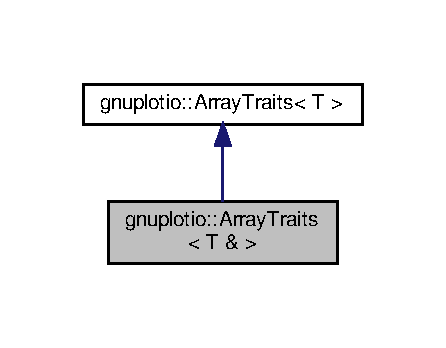
\includegraphics[width=214pt]{classgnuplotio_1_1ArrayTraits_3_01T_01_6_01_4__inherit__graph}
\end{center}
\end{figure}


Collaboration diagram for gnuplotio\+:\+:Array\+Traits$<$ T \& $>$\+:\nopagebreak
\begin{figure}[H]
\begin{center}
\leavevmode
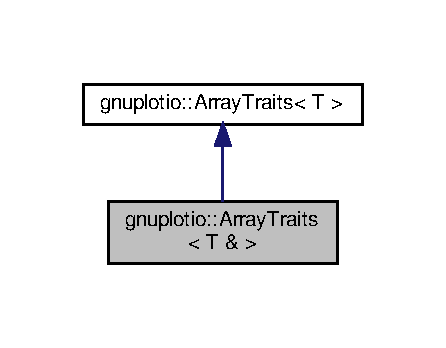
\includegraphics[width=214pt]{classgnuplotio_1_1ArrayTraits_3_01T_01_6_01_4__coll__graph}
\end{center}
\end{figure}
\subsection*{Additional Inherited Members}


The documentation for this class was generated from the following file\+:\begin{DoxyCompactItemize}
\item 
include/gnuplot-\/iostream.\+h\end{DoxyCompactItemize}

\hypertarget{classgnuplotio_1_1ArrayTraits_3_01T_00_01typename_01boost_1_1enable__if_3_01boost_1_1mpl_1_1and_371638f7d82cde4b7a8a064d0797371a}{}\section{gnuplotio\+:\+:Array\+Traits$<$ T, typename boost\+:\+:enable\+\_\+if$<$ boost\+:\+:mpl\+:\+:and\+\_\+$<$ is\+\_\+boost\+\_\+tuple$<$ T $>$, boost\+:\+:mpl\+:\+:not\+\_\+$<$ is\+\_\+boost\+\_\+tuple\+\_\+nulltype$<$ typename T\+:\+:tail\+\_\+type $>$ $>$ $>$ $>$\+:\+:type $>$ Class Template Reference}
\label{classgnuplotio_1_1ArrayTraits_3_01T_00_01typename_01boost_1_1enable__if_3_01boost_1_1mpl_1_1and_371638f7d82cde4b7a8a064d0797371a}\index{gnuplotio\+::\+Array\+Traits$<$ T, typename boost\+::enable\+\_\+if$<$ boost\+::mpl\+::and\+\_\+$<$ is\+\_\+boost\+\_\+tuple$<$ T $>$, boost\+::mpl\+::not\+\_\+$<$ is\+\_\+boost\+\_\+tuple\+\_\+nulltype$<$ typename T\+::tail\+\_\+type $>$ $>$ $>$ $>$\+::type $>$@{gnuplotio\+::\+Array\+Traits$<$ T, typename boost\+::enable\+\_\+if$<$ boost\+::mpl\+::and\+\_\+$<$ is\+\_\+boost\+\_\+tuple$<$ T $>$, boost\+::mpl\+::not\+\_\+$<$ is\+\_\+boost\+\_\+tuple\+\_\+nulltype$<$ typename T\+::tail\+\_\+type $>$ $>$ $>$ $>$\+::type $>$}}


Inheritance diagram for gnuplotio\+:\+:Array\+Traits$<$ T, typename boost\+:\+:enable\+\_\+if$<$ boost\+:\+:mpl\+:\+:and\+\_\+$<$ is\+\_\+boost\+\_\+tuple$<$ T $>$, boost\+:\+:mpl\+:\+:not\+\_\+$<$ is\+\_\+boost\+\_\+tuple\+\_\+nulltype$<$ typename T\+:\+:tail\+\_\+type $>$ $>$ $>$ $>$\+:\+:type $>$\+:\nopagebreak
\begin{figure}[H]
\begin{center}
\leavevmode
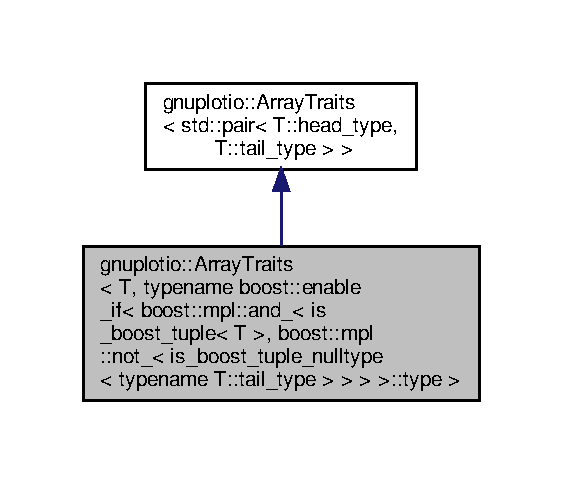
\includegraphics[width=270pt]{classgnuplotio_1_1ArrayTraits_3_01T_00_01typename_01boost_1_1enable__if_3_01boost_1_1mpl_1_1and_691fea0d25810f91cf71bd7a5d3b39c5}
\end{center}
\end{figure}


Collaboration diagram for gnuplotio\+:\+:Array\+Traits$<$ T, typename boost\+:\+:enable\+\_\+if$<$ boost\+:\+:mpl\+:\+:and\+\_\+$<$ is\+\_\+boost\+\_\+tuple$<$ T $>$, boost\+:\+:mpl\+:\+:not\+\_\+$<$ is\+\_\+boost\+\_\+tuple\+\_\+nulltype$<$ typename T\+:\+:tail\+\_\+type $>$ $>$ $>$ $>$\+:\+:type $>$\+:\nopagebreak
\begin{figure}[H]
\begin{center}
\leavevmode
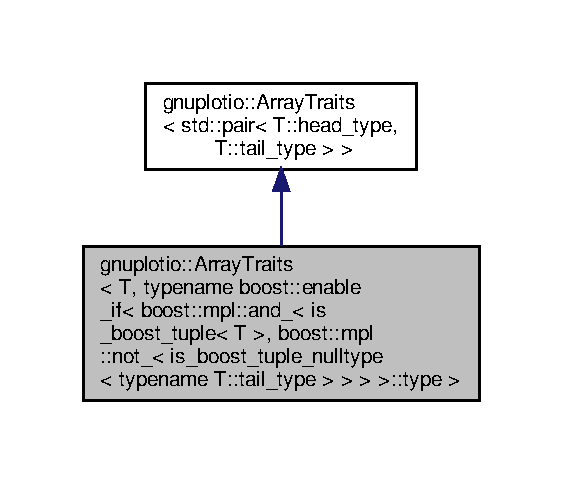
\includegraphics[width=270pt]{classgnuplotio_1_1ArrayTraits_3_01T_00_01typename_01boost_1_1enable__if_3_01boost_1_1mpl_1_1and_5c5b3f7103a9f155bd15ec6df70697d0}
\end{center}
\end{figure}
\subsection*{Public Types}
\begin{DoxyCompactItemize}
\item 
\mbox{\Hypertarget{classgnuplotio_1_1ArrayTraits_3_01T_00_01typename_01boost_1_1enable__if_3_01boost_1_1mpl_1_1and_371638f7d82cde4b7a8a064d0797371a_ab56761f05b74be318cc7becbc59348df}\label{classgnuplotio_1_1ArrayTraits_3_01T_00_01typename_01boost_1_1enable__if_3_01boost_1_1mpl_1_1and_371638f7d82cde4b7a8a064d0797371a_ab56761f05b74be318cc7becbc59348df}} 
typedef T\+::head\+\_\+type {\bfseries HT}
\item 
\mbox{\Hypertarget{classgnuplotio_1_1ArrayTraits_3_01T_00_01typename_01boost_1_1enable__if_3_01boost_1_1mpl_1_1and_371638f7d82cde4b7a8a064d0797371a_a16316f598ab57b0b7ceea99dcd34632e}\label{classgnuplotio_1_1ArrayTraits_3_01T_00_01typename_01boost_1_1enable__if_3_01boost_1_1mpl_1_1and_371638f7d82cde4b7a8a064d0797371a_a16316f598ab57b0b7ceea99dcd34632e}} 
typedef T\+::tail\+\_\+type {\bfseries TT}
\item 
\mbox{\Hypertarget{classgnuplotio_1_1ArrayTraits_3_01T_00_01typename_01boost_1_1enable__if_3_01boost_1_1mpl_1_1and_371638f7d82cde4b7a8a064d0797371a_aad44f59a1d618b863442a9fdaa83d142}\label{classgnuplotio_1_1ArrayTraits_3_01T_00_01typename_01boost_1_1enable__if_3_01boost_1_1mpl_1_1and_371638f7d82cde4b7a8a064d0797371a_aad44f59a1d618b863442a9fdaa83d142}} 
typedef \hyperlink{classgnuplotio_1_1ArrayTraits}{Array\+Traits}$<$ typename std\+::pair$<$ HT, TT $>$ $>$ {\bfseries parent}
\end{DoxyCompactItemize}
\subsection*{Static Public Member Functions}
\begin{DoxyCompactItemize}
\item 
\mbox{\Hypertarget{classgnuplotio_1_1ArrayTraits_3_01T_00_01typename_01boost_1_1enable__if_3_01boost_1_1mpl_1_1and_371638f7d82cde4b7a8a064d0797371a_aec07e01edbb46f5f283d5b6af068c0f2}\label{classgnuplotio_1_1ArrayTraits_3_01T_00_01typename_01boost_1_1enable__if_3_01boost_1_1mpl_1_1and_371638f7d82cde4b7a8a064d0797371a_aec07e01edbb46f5f283d5b6af068c0f2}} 
static \hyperlink{structgnuplotio_1_1Error__WasNotContainer}{parent\+::range\+\_\+type} {\bfseries get\+\_\+range} (const T \&arg)
\end{DoxyCompactItemize}
\subsection*{Additional Inherited Members}


The documentation for this class was generated from the following file\+:\begin{DoxyCompactItemize}
\item 
include/gnuplot-\/iostream.\+h\end{DoxyCompactItemize}

\hypertarget{classgnuplotio_1_1ArrayTraits_3_01T_00_01typename_01boost_1_1enable__if_3_01boost_1_1mpl_1_1and_d5bfbd58f322d0a74d370034dff1881d}{}\section{gnuplotio\+:\+:Array\+Traits$<$ T, typename boost\+:\+:enable\+\_\+if$<$ boost\+:\+:mpl\+:\+:and\+\_\+$<$ is\+\_\+boost\+\_\+tuple$<$ T $>$, is\+\_\+boost\+\_\+tuple\+\_\+nulltype$<$ typename T\+:\+:tail\+\_\+type $>$ $>$ $>$\+:\+:type $>$ Class Template Reference}
\label{classgnuplotio_1_1ArrayTraits_3_01T_00_01typename_01boost_1_1enable__if_3_01boost_1_1mpl_1_1and_d5bfbd58f322d0a74d370034dff1881d}\index{gnuplotio\+::\+Array\+Traits$<$ T, typename boost\+::enable\+\_\+if$<$ boost\+::mpl\+::and\+\_\+$<$ is\+\_\+boost\+\_\+tuple$<$ T $>$, is\+\_\+boost\+\_\+tuple\+\_\+nulltype$<$ typename T\+::tail\+\_\+type $>$ $>$ $>$\+::type $>$@{gnuplotio\+::\+Array\+Traits$<$ T, typename boost\+::enable\+\_\+if$<$ boost\+::mpl\+::and\+\_\+$<$ is\+\_\+boost\+\_\+tuple$<$ T $>$, is\+\_\+boost\+\_\+tuple\+\_\+nulltype$<$ typename T\+::tail\+\_\+type $>$ $>$ $>$\+::type $>$}}


Inheritance diagram for gnuplotio\+:\+:Array\+Traits$<$ T, typename boost\+:\+:enable\+\_\+if$<$ boost\+:\+:mpl\+:\+:and\+\_\+$<$ is\+\_\+boost\+\_\+tuple$<$ T $>$, is\+\_\+boost\+\_\+tuple\+\_\+nulltype$<$ typename T\+:\+:tail\+\_\+type $>$ $>$ $>$\+:\+:type $>$\+:\nopagebreak
\begin{figure}[H]
\begin{center}
\leavevmode
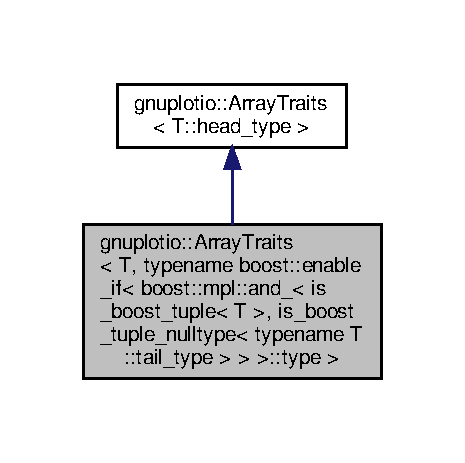
\includegraphics[width=223pt]{classgnuplotio_1_1ArrayTraits_3_01T_00_01typename_01boost_1_1enable__if_3_01boost_1_1mpl_1_1and_aeaabfa162f172ea27fc7936200f6db1}
\end{center}
\end{figure}


Collaboration diagram for gnuplotio\+:\+:Array\+Traits$<$ T, typename boost\+:\+:enable\+\_\+if$<$ boost\+:\+:mpl\+:\+:and\+\_\+$<$ is\+\_\+boost\+\_\+tuple$<$ T $>$, is\+\_\+boost\+\_\+tuple\+\_\+nulltype$<$ typename T\+:\+:tail\+\_\+type $>$ $>$ $>$\+:\+:type $>$\+:\nopagebreak
\begin{figure}[H]
\begin{center}
\leavevmode
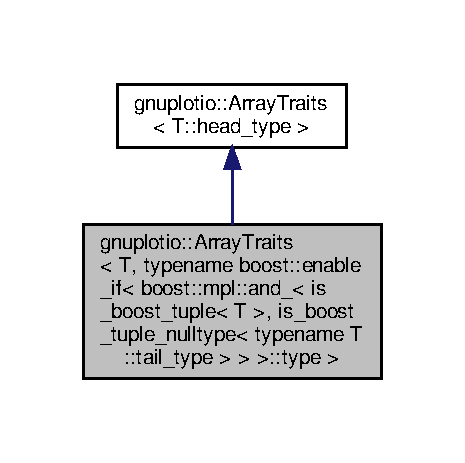
\includegraphics[width=223pt]{classgnuplotio_1_1ArrayTraits_3_01T_00_01typename_01boost_1_1enable__if_3_01boost_1_1mpl_1_1and_664a33c2200adb4ffe25ffcb83c434f5}
\end{center}
\end{figure}
\subsection*{Static Public Member Functions}
\begin{DoxyCompactItemize}
\item 
\mbox{\Hypertarget{classgnuplotio_1_1ArrayTraits_3_01T_00_01typename_01boost_1_1enable__if_3_01boost_1_1mpl_1_1and_d5bfbd58f322d0a74d370034dff1881d_ad0485dd16a9d54a4eb75bf3e75b1facd}\label{classgnuplotio_1_1ArrayTraits_3_01T_00_01typename_01boost_1_1enable__if_3_01boost_1_1mpl_1_1and_d5bfbd58f322d0a74d370034dff1881d_ad0485dd16a9d54a4eb75bf3e75b1facd}} 
static \hyperlink{structgnuplotio_1_1Error__WasNotContainer}{parent\+::range\+\_\+type} {\bfseries get\+\_\+range} (const T \&arg)
\end{DoxyCompactItemize}
\subsection*{Additional Inherited Members}


The documentation for this class was generated from the following file\+:\begin{DoxyCompactItemize}
\item 
include/gnuplot-\/iostream.\+h\end{DoxyCompactItemize}

\hypertarget{classgnuplotio_1_1ArrayTraits_3_01T_00_01typename_01boost_1_1enable__if_3_01is__like__stl__conta99f8c9e80e271bc1ed047cdd05794af4}{}\section{gnuplotio\+:\+:Array\+Traits$<$ T, typename boost\+:\+:enable\+\_\+if$<$ is\+\_\+like\+\_\+stl\+\_\+container$<$ T $>$ $>$\+:\+:type $>$ Class Template Reference}
\label{classgnuplotio_1_1ArrayTraits_3_01T_00_01typename_01boost_1_1enable__if_3_01is__like__stl__conta99f8c9e80e271bc1ed047cdd05794af4}\index{gnuplotio\+::\+Array\+Traits$<$ T, typename boost\+::enable\+\_\+if$<$ is\+\_\+like\+\_\+stl\+\_\+container$<$ T $>$ $>$\+::type $>$@{gnuplotio\+::\+Array\+Traits$<$ T, typename boost\+::enable\+\_\+if$<$ is\+\_\+like\+\_\+stl\+\_\+container$<$ T $>$ $>$\+::type $>$}}


Inheritance diagram for gnuplotio\+:\+:Array\+Traits$<$ T, typename boost\+:\+:enable\+\_\+if$<$ is\+\_\+like\+\_\+stl\+\_\+container$<$ T $>$ $>$\+:\+:type $>$\+:\nopagebreak
\begin{figure}[H]
\begin{center}
\leavevmode
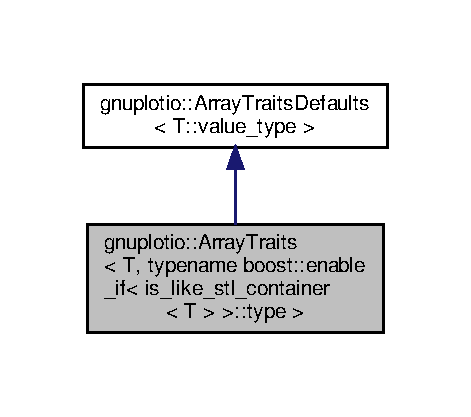
\includegraphics[width=226pt]{classgnuplotio_1_1ArrayTraits_3_01T_00_01typename_01boost_1_1enable__if_3_01is__like__stl__conta5c9a0526d4b8f3b59efa70a3e03b094a}
\end{center}
\end{figure}


Collaboration diagram for gnuplotio\+:\+:Array\+Traits$<$ T, typename boost\+:\+:enable\+\_\+if$<$ is\+\_\+like\+\_\+stl\+\_\+container$<$ T $>$ $>$\+:\+:type $>$\+:\nopagebreak
\begin{figure}[H]
\begin{center}
\leavevmode
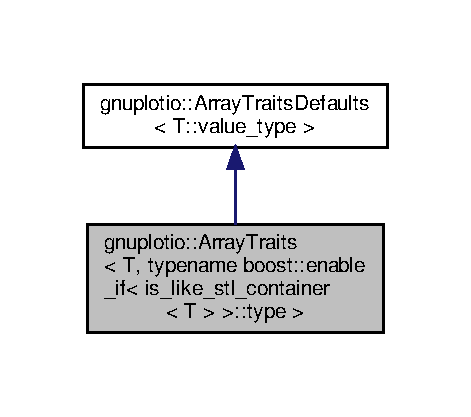
\includegraphics[width=226pt]{classgnuplotio_1_1ArrayTraits_3_01T_00_01typename_01boost_1_1enable__if_3_01is__like__stl__conta4401937b8251776f9383339a7f86e7bc}
\end{center}
\end{figure}
\subsection*{Public Types}
\begin{DoxyCompactItemize}
\item 
\mbox{\Hypertarget{classgnuplotio_1_1ArrayTraits_3_01T_00_01typename_01boost_1_1enable__if_3_01is__like__stl__conta99f8c9e80e271bc1ed047cdd05794af4_ab702072abbe018bbc90b9967ca8c4b42}\label{classgnuplotio_1_1ArrayTraits_3_01T_00_01typename_01boost_1_1enable__if_3_01is__like__stl__conta99f8c9e80e271bc1ed047cdd05794af4_ab702072abbe018bbc90b9967ca8c4b42}} 
typedef \hyperlink{classgnuplotio_1_1IteratorRange}{Iterator\+Range}$<$ typename T\+::const\+\_\+iterator, typename T\+::value\+\_\+type $>$ {\bfseries range\+\_\+type}
\end{DoxyCompactItemize}
\subsection*{Static Public Member Functions}
\begin{DoxyCompactItemize}
\item 
\mbox{\Hypertarget{classgnuplotio_1_1ArrayTraits_3_01T_00_01typename_01boost_1_1enable__if_3_01is__like__stl__conta99f8c9e80e271bc1ed047cdd05794af4_a89d4150ab3c479cde972071a10acd27b}\label{classgnuplotio_1_1ArrayTraits_3_01T_00_01typename_01boost_1_1enable__if_3_01is__like__stl__conta99f8c9e80e271bc1ed047cdd05794af4_a89d4150ab3c479cde972071a10acd27b}} 
static \hyperlink{classgnuplotio_1_1IteratorRange}{range\+\_\+type} {\bfseries get\+\_\+range} (const T \&arg)
\end{DoxyCompactItemize}
\subsection*{Additional Inherited Members}


The documentation for this class was generated from the following file\+:\begin{DoxyCompactItemize}
\item 
include/gnuplot-\/iostream.\+h\end{DoxyCompactItemize}

\hypertarget{classgnuplotio_1_1ArrayTraits_3_01T[N]_4}{}\section{gnuplotio\+:\+:Array\+Traits$<$ T\mbox{[}N\mbox{]}$>$ Class Template Reference}
\label{classgnuplotio_1_1ArrayTraits_3_01T[N]_4}\index{gnuplotio\+::\+Array\+Traits$<$ T\mbox{[}N\mbox{]}$>$@{gnuplotio\+::\+Array\+Traits$<$ T[N]$>$}}


Inheritance diagram for gnuplotio\+:\+:Array\+Traits$<$ T\mbox{[}N\mbox{]}$>$\+:\nopagebreak
\begin{figure}[H]
\begin{center}
\leavevmode
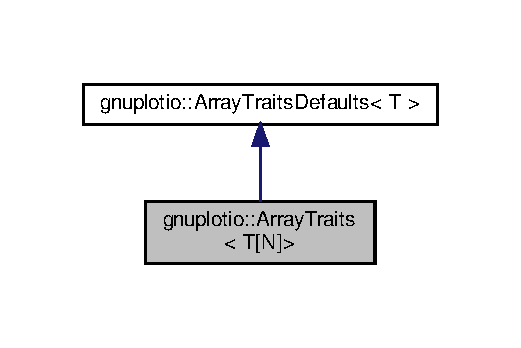
\includegraphics[width=250pt]{classgnuplotio_1_1ArrayTraits_3_01T[N]_4__inherit__graph}
\end{center}
\end{figure}


Collaboration diagram for gnuplotio\+:\+:Array\+Traits$<$ T\mbox{[}N\mbox{]}$>$\+:\nopagebreak
\begin{figure}[H]
\begin{center}
\leavevmode
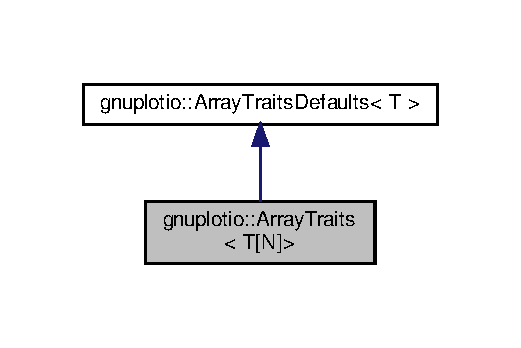
\includegraphics[width=250pt]{classgnuplotio_1_1ArrayTraits_3_01T[N]_4__coll__graph}
\end{center}
\end{figure}
\subsection*{Public Types}
\begin{DoxyCompactItemize}
\item 
\mbox{\Hypertarget{classgnuplotio_1_1ArrayTraits_3_01T[N]_4_a926f3c3d14fbe82aab7b70ccc16d20fb}\label{classgnuplotio_1_1ArrayTraits_3_01T[N]_4_a926f3c3d14fbe82aab7b70ccc16d20fb}} 
typedef \hyperlink{classgnuplotio_1_1IteratorRange}{Iterator\+Range}$<$ const T $\ast$, T $>$ {\bfseries range\+\_\+type}
\end{DoxyCompactItemize}
\subsection*{Static Public Member Functions}
\begin{DoxyCompactItemize}
\item 
\mbox{\Hypertarget{classgnuplotio_1_1ArrayTraits_3_01T[N]_4_adc9c1ce6da4923418f367e08c150a928}\label{classgnuplotio_1_1ArrayTraits_3_01T[N]_4_adc9c1ce6da4923418f367e08c150a928}} 
static \hyperlink{classgnuplotio_1_1IteratorRange}{range\+\_\+type} {\bfseries get\+\_\+range} (const T(\&arg)\mbox{[}N\mbox{]})
\end{DoxyCompactItemize}
\subsection*{Additional Inherited Members}


The documentation for this class was generated from the following file\+:\begin{DoxyCompactItemize}
\item 
include/gnuplot-\/iostream.\+h\end{DoxyCompactItemize}

\hypertarget{classgnuplotio_1_1ArrayTraitsDefaults}{}\section{gnuplotio\+:\+:Array\+Traits\+Defaults$<$ V $>$ Class Template Reference}
\label{classgnuplotio_1_1ArrayTraitsDefaults}\index{gnuplotio\+::\+Array\+Traits\+Defaults$<$ V $>$@{gnuplotio\+::\+Array\+Traits\+Defaults$<$ V $>$}}
\subsection*{Public Types}
\begin{DoxyCompactItemize}
\item 
\mbox{\Hypertarget{classgnuplotio_1_1ArrayTraitsDefaults_ad7a9e8d19419fabe2ab9cc1b76c9965b}\label{classgnuplotio_1_1ArrayTraitsDefaults_ad7a9e8d19419fabe2ab9cc1b76c9965b}} 
typedef V {\bfseries value\+\_\+type}
\end{DoxyCompactItemize}
\subsection*{Static Public Attributes}
\begin{DoxyCompactItemize}
\item 
\mbox{\Hypertarget{classgnuplotio_1_1ArrayTraitsDefaults_a57bab5bf3617f0ee66fdd4dcb751aa21}\label{classgnuplotio_1_1ArrayTraitsDefaults_a57bab5bf3617f0ee66fdd4dcb751aa21}} 
static const bool {\bfseries is\+\_\+container} = true
\item 
\mbox{\Hypertarget{classgnuplotio_1_1ArrayTraitsDefaults_ac8d430cba6ceefc6f52706455f12a0e8}\label{classgnuplotio_1_1ArrayTraitsDefaults_ac8d430cba6ceefc6f52706455f12a0e8}} 
static const bool {\bfseries allow\+\_\+auto\+\_\+unwrap} = true
\item 
\mbox{\Hypertarget{classgnuplotio_1_1ArrayTraitsDefaults_ac51367f5da9096249b162af1496e36ab}\label{classgnuplotio_1_1ArrayTraitsDefaults_ac51367f5da9096249b162af1496e36ab}} 
static const size\+\_\+t {\bfseries depth} = \hyperlink{classgnuplotio_1_1ArrayTraits}{Array\+Traits}$<$V$>$\+::depth + 1
\end{DoxyCompactItemize}


The documentation for this class was generated from the following file\+:\begin{DoxyCompactItemize}
\item 
include/gnuplot-\/iostream.\+h\end{DoxyCompactItemize}

\hypertarget{structgnuplotio_1_1BinarySender}{}\section{gnuplotio\+:\+:Binary\+Sender$<$ T, Enable $>$ Struct Template Reference}
\label{structgnuplotio_1_1BinarySender}\index{gnuplotio\+::\+Binary\+Sender$<$ T, Enable $>$@{gnuplotio\+::\+Binary\+Sender$<$ T, Enable $>$}}
\subsection*{Public Member Functions}
\begin{DoxyCompactItemize}
\item 
\mbox{\Hypertarget{structgnuplotio_1_1BinarySender_ad964fa720473ff517cfb461361f645c8}\label{structgnuplotio_1_1BinarySender_ad964fa720473ff517cfb461361f645c8}} 
{\bfseries G\+N\+U\+P\+L\+O\+T\+\_\+\+S\+T\+A\+T\+I\+C\+\_\+\+A\+S\+S\+E\+R\+T\+\_\+\+M\+SG} ((sizeof(T)==0), \char`\"{}Binary\+Sender class not specialized for this type\char`\"{})
\end{DoxyCompactItemize}
\subsection*{Static Public Member Functions}
\begin{DoxyCompactItemize}
\item 
\mbox{\Hypertarget{structgnuplotio_1_1BinarySender_a4b5dd22b7679c4f0ce4d8e75b36c8a21}\label{structgnuplotio_1_1BinarySender_a4b5dd22b7679c4f0ce4d8e75b36c8a21}} 
static void {\bfseries send} (std\+::ostream \&stream, const T \&v)
\end{DoxyCompactItemize}


The documentation for this struct was generated from the following file\+:\begin{DoxyCompactItemize}
\item 
include/gnuplot-\/iostream.\+h\end{DoxyCompactItemize}

\hypertarget{structgnuplotio_1_1BinarySender_3_01boost_1_1int16__t_01_4}{}\section{gnuplotio\+:\+:Binary\+Sender$<$ boost\+:\+:int16\+\_\+t $>$ Struct Template Reference}
\label{structgnuplotio_1_1BinarySender_3_01boost_1_1int16__t_01_4}\index{gnuplotio\+::\+Binary\+Sender$<$ boost\+::int16\+\_\+t $>$@{gnuplotio\+::\+Binary\+Sender$<$ boost\+::int16\+\_\+t $>$}}


Inheritance diagram for gnuplotio\+:\+:Binary\+Sender$<$ boost\+:\+:int16\+\_\+t $>$\+:\nopagebreak
\begin{figure}[H]
\begin{center}
\leavevmode
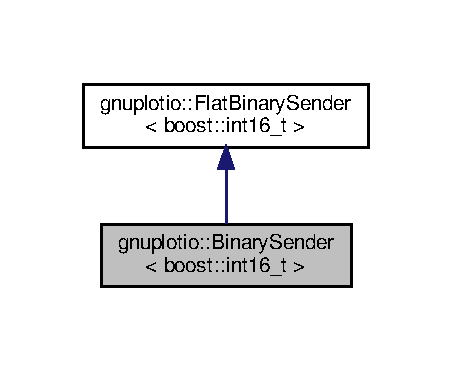
\includegraphics[width=217pt]{structgnuplotio_1_1BinarySender_3_01boost_1_1int16__t_01_4__inherit__graph}
\end{center}
\end{figure}


Collaboration diagram for gnuplotio\+:\+:Binary\+Sender$<$ boost\+:\+:int16\+\_\+t $>$\+:\nopagebreak
\begin{figure}[H]
\begin{center}
\leavevmode
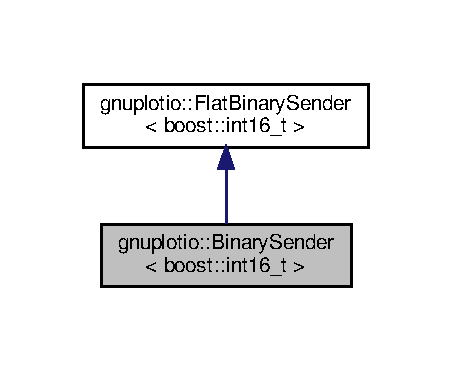
\includegraphics[width=217pt]{structgnuplotio_1_1BinarySender_3_01boost_1_1int16__t_01_4__coll__graph}
\end{center}
\end{figure}
\subsection*{Additional Inherited Members}


The documentation for this struct was generated from the following file\+:\begin{DoxyCompactItemize}
\item 
include/gnuplot-\/iostream.\+h\end{DoxyCompactItemize}

\hypertarget{structgnuplotio_1_1BinarySender_3_01boost_1_1int32__t_01_4}{}\section{gnuplotio\+:\+:Binary\+Sender$<$ boost\+:\+:int32\+\_\+t $>$ Struct Template Reference}
\label{structgnuplotio_1_1BinarySender_3_01boost_1_1int32__t_01_4}\index{gnuplotio\+::\+Binary\+Sender$<$ boost\+::int32\+\_\+t $>$@{gnuplotio\+::\+Binary\+Sender$<$ boost\+::int32\+\_\+t $>$}}


Inheritance diagram for gnuplotio\+:\+:Binary\+Sender$<$ boost\+:\+:int32\+\_\+t $>$\+:\nopagebreak
\begin{figure}[H]
\begin{center}
\leavevmode
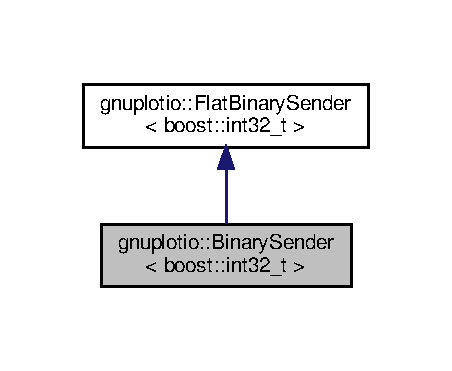
\includegraphics[width=217pt]{structgnuplotio_1_1BinarySender_3_01boost_1_1int32__t_01_4__inherit__graph}
\end{center}
\end{figure}


Collaboration diagram for gnuplotio\+:\+:Binary\+Sender$<$ boost\+:\+:int32\+\_\+t $>$\+:\nopagebreak
\begin{figure}[H]
\begin{center}
\leavevmode
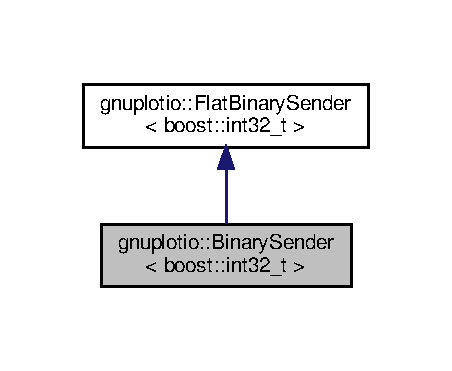
\includegraphics[width=217pt]{structgnuplotio_1_1BinarySender_3_01boost_1_1int32__t_01_4__coll__graph}
\end{center}
\end{figure}
\subsection*{Additional Inherited Members}


The documentation for this struct was generated from the following file\+:\begin{DoxyCompactItemize}
\item 
include/gnuplot-\/iostream.\+h\end{DoxyCompactItemize}

\hypertarget{structgnuplotio_1_1BinarySender_3_01boost_1_1int64__t_01_4}{}\section{gnuplotio\+:\+:Binary\+Sender$<$ boost\+:\+:int64\+\_\+t $>$ Struct Template Reference}
\label{structgnuplotio_1_1BinarySender_3_01boost_1_1int64__t_01_4}\index{gnuplotio\+::\+Binary\+Sender$<$ boost\+::int64\+\_\+t $>$@{gnuplotio\+::\+Binary\+Sender$<$ boost\+::int64\+\_\+t $>$}}


Inheritance diagram for gnuplotio\+:\+:Binary\+Sender$<$ boost\+:\+:int64\+\_\+t $>$\+:\nopagebreak
\begin{figure}[H]
\begin{center}
\leavevmode
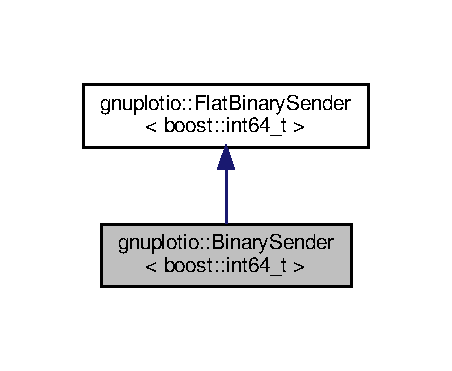
\includegraphics[width=217pt]{structgnuplotio_1_1BinarySender_3_01boost_1_1int64__t_01_4__inherit__graph}
\end{center}
\end{figure}


Collaboration diagram for gnuplotio\+:\+:Binary\+Sender$<$ boost\+:\+:int64\+\_\+t $>$\+:\nopagebreak
\begin{figure}[H]
\begin{center}
\leavevmode
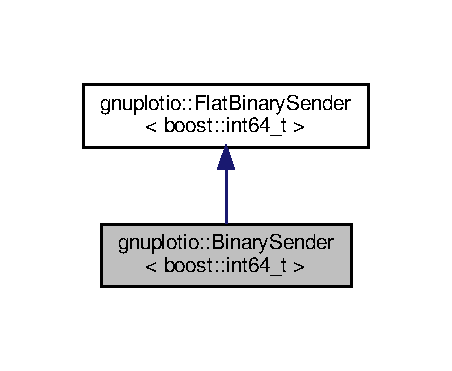
\includegraphics[width=217pt]{structgnuplotio_1_1BinarySender_3_01boost_1_1int64__t_01_4__coll__graph}
\end{center}
\end{figure}
\subsection*{Additional Inherited Members}


The documentation for this struct was generated from the following file\+:\begin{DoxyCompactItemize}
\item 
include/gnuplot-\/iostream.\+h\end{DoxyCompactItemize}

\hypertarget{structgnuplotio_1_1BinarySender_3_01boost_1_1int8__t_01_4}{}\section{gnuplotio\+:\+:Binary\+Sender$<$ boost\+:\+:int8\+\_\+t $>$ Struct Template Reference}
\label{structgnuplotio_1_1BinarySender_3_01boost_1_1int8__t_01_4}\index{gnuplotio\+::\+Binary\+Sender$<$ boost\+::int8\+\_\+t $>$@{gnuplotio\+::\+Binary\+Sender$<$ boost\+::int8\+\_\+t $>$}}


Inheritance diagram for gnuplotio\+:\+:Binary\+Sender$<$ boost\+:\+:int8\+\_\+t $>$\+:\nopagebreak
\begin{figure}[H]
\begin{center}
\leavevmode
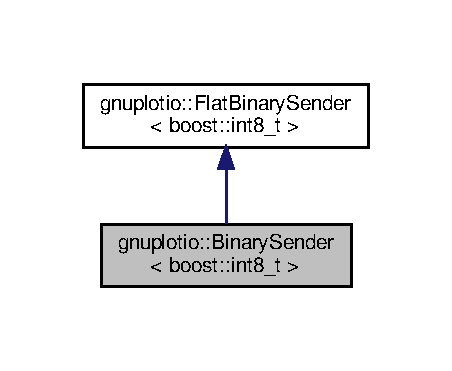
\includegraphics[width=217pt]{structgnuplotio_1_1BinarySender_3_01boost_1_1int8__t_01_4__inherit__graph}
\end{center}
\end{figure}


Collaboration diagram for gnuplotio\+:\+:Binary\+Sender$<$ boost\+:\+:int8\+\_\+t $>$\+:\nopagebreak
\begin{figure}[H]
\begin{center}
\leavevmode
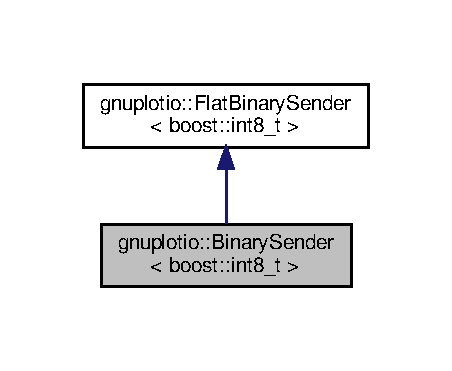
\includegraphics[width=217pt]{structgnuplotio_1_1BinarySender_3_01boost_1_1int8__t_01_4__coll__graph}
\end{center}
\end{figure}
\subsection*{Additional Inherited Members}


The documentation for this struct was generated from the following file\+:\begin{DoxyCompactItemize}
\item 
include/gnuplot-\/iostream.\+h\end{DoxyCompactItemize}

\hypertarget{structgnuplotio_1_1BinarySender_3_01boost_1_1uint16__t_01_4}{}\section{gnuplotio\+:\+:Binary\+Sender$<$ boost\+:\+:uint16\+\_\+t $>$ Struct Template Reference}
\label{structgnuplotio_1_1BinarySender_3_01boost_1_1uint16__t_01_4}\index{gnuplotio\+::\+Binary\+Sender$<$ boost\+::uint16\+\_\+t $>$@{gnuplotio\+::\+Binary\+Sender$<$ boost\+::uint16\+\_\+t $>$}}


Inheritance diagram for gnuplotio\+:\+:Binary\+Sender$<$ boost\+:\+:uint16\+\_\+t $>$\+:\nopagebreak
\begin{figure}[H]
\begin{center}
\leavevmode
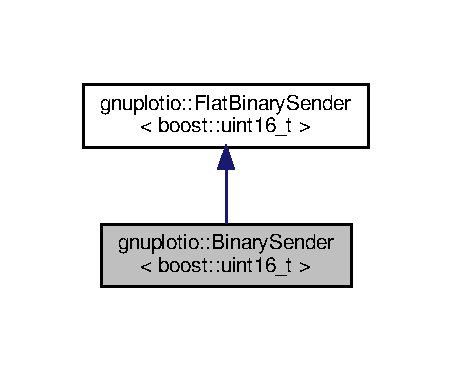
\includegraphics[width=217pt]{structgnuplotio_1_1BinarySender_3_01boost_1_1uint16__t_01_4__inherit__graph}
\end{center}
\end{figure}


Collaboration diagram for gnuplotio\+:\+:Binary\+Sender$<$ boost\+:\+:uint16\+\_\+t $>$\+:\nopagebreak
\begin{figure}[H]
\begin{center}
\leavevmode
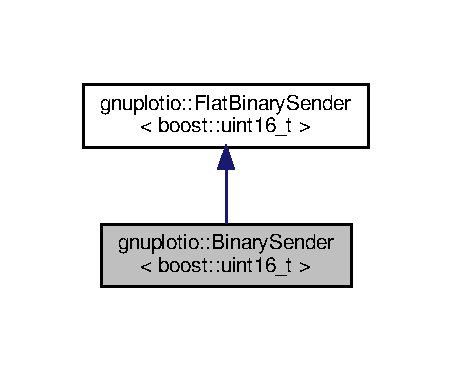
\includegraphics[width=217pt]{structgnuplotio_1_1BinarySender_3_01boost_1_1uint16__t_01_4__coll__graph}
\end{center}
\end{figure}
\subsection*{Additional Inherited Members}


The documentation for this struct was generated from the following file\+:\begin{DoxyCompactItemize}
\item 
include/gnuplot-\/iostream.\+h\end{DoxyCompactItemize}

\hypertarget{structgnuplotio_1_1BinarySender_3_01boost_1_1uint32__t_01_4}{}\section{gnuplotio\+:\+:Binary\+Sender$<$ boost\+:\+:uint32\+\_\+t $>$ Struct Template Reference}
\label{structgnuplotio_1_1BinarySender_3_01boost_1_1uint32__t_01_4}\index{gnuplotio\+::\+Binary\+Sender$<$ boost\+::uint32\+\_\+t $>$@{gnuplotio\+::\+Binary\+Sender$<$ boost\+::uint32\+\_\+t $>$}}


Inheritance diagram for gnuplotio\+:\+:Binary\+Sender$<$ boost\+:\+:uint32\+\_\+t $>$\+:\nopagebreak
\begin{figure}[H]
\begin{center}
\leavevmode
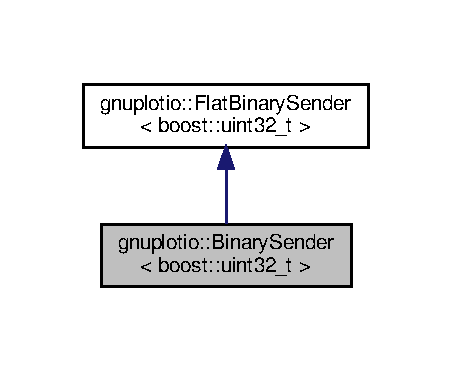
\includegraphics[width=217pt]{structgnuplotio_1_1BinarySender_3_01boost_1_1uint32__t_01_4__inherit__graph}
\end{center}
\end{figure}


Collaboration diagram for gnuplotio\+:\+:Binary\+Sender$<$ boost\+:\+:uint32\+\_\+t $>$\+:\nopagebreak
\begin{figure}[H]
\begin{center}
\leavevmode
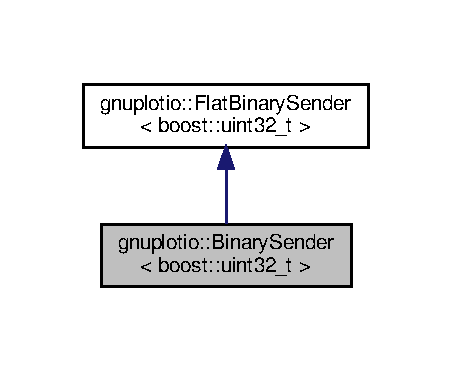
\includegraphics[width=217pt]{structgnuplotio_1_1BinarySender_3_01boost_1_1uint32__t_01_4__coll__graph}
\end{center}
\end{figure}
\subsection*{Additional Inherited Members}


The documentation for this struct was generated from the following file\+:\begin{DoxyCompactItemize}
\item 
include/gnuplot-\/iostream.\+h\end{DoxyCompactItemize}

\hypertarget{structgnuplotio_1_1BinarySender_3_01boost_1_1uint64__t_01_4}{}\section{gnuplotio\+:\+:Binary\+Sender$<$ boost\+:\+:uint64\+\_\+t $>$ Struct Template Reference}
\label{structgnuplotio_1_1BinarySender_3_01boost_1_1uint64__t_01_4}\index{gnuplotio\+::\+Binary\+Sender$<$ boost\+::uint64\+\_\+t $>$@{gnuplotio\+::\+Binary\+Sender$<$ boost\+::uint64\+\_\+t $>$}}


Inheritance diagram for gnuplotio\+:\+:Binary\+Sender$<$ boost\+:\+:uint64\+\_\+t $>$\+:\nopagebreak
\begin{figure}[H]
\begin{center}
\leavevmode
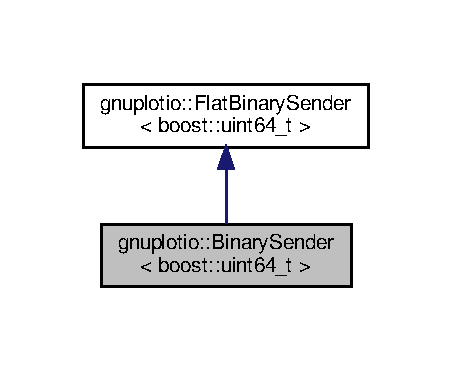
\includegraphics[width=217pt]{structgnuplotio_1_1BinarySender_3_01boost_1_1uint64__t_01_4__inherit__graph}
\end{center}
\end{figure}


Collaboration diagram for gnuplotio\+:\+:Binary\+Sender$<$ boost\+:\+:uint64\+\_\+t $>$\+:\nopagebreak
\begin{figure}[H]
\begin{center}
\leavevmode
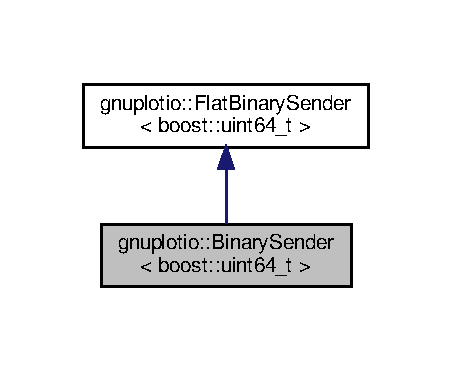
\includegraphics[width=217pt]{structgnuplotio_1_1BinarySender_3_01boost_1_1uint64__t_01_4__coll__graph}
\end{center}
\end{figure}
\subsection*{Additional Inherited Members}


The documentation for this struct was generated from the following file\+:\begin{DoxyCompactItemize}
\item 
include/gnuplot-\/iostream.\+h\end{DoxyCompactItemize}

\hypertarget{structgnuplotio_1_1BinarySender_3_01boost_1_1uint8__t_01_4}{}\section{gnuplotio\+:\+:Binary\+Sender$<$ boost\+:\+:uint8\+\_\+t $>$ Struct Template Reference}
\label{structgnuplotio_1_1BinarySender_3_01boost_1_1uint8__t_01_4}\index{gnuplotio\+::\+Binary\+Sender$<$ boost\+::uint8\+\_\+t $>$@{gnuplotio\+::\+Binary\+Sender$<$ boost\+::uint8\+\_\+t $>$}}


Inheritance diagram for gnuplotio\+:\+:Binary\+Sender$<$ boost\+:\+:uint8\+\_\+t $>$\+:\nopagebreak
\begin{figure}[H]
\begin{center}
\leavevmode
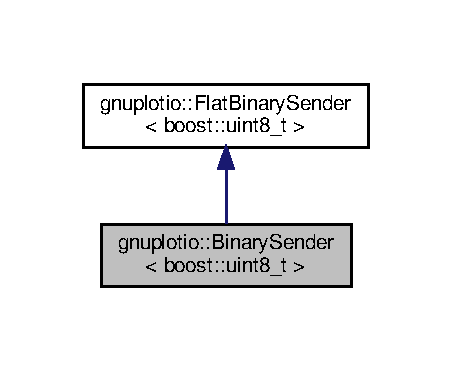
\includegraphics[width=217pt]{structgnuplotio_1_1BinarySender_3_01boost_1_1uint8__t_01_4__inherit__graph}
\end{center}
\end{figure}


Collaboration diagram for gnuplotio\+:\+:Binary\+Sender$<$ boost\+:\+:uint8\+\_\+t $>$\+:\nopagebreak
\begin{figure}[H]
\begin{center}
\leavevmode
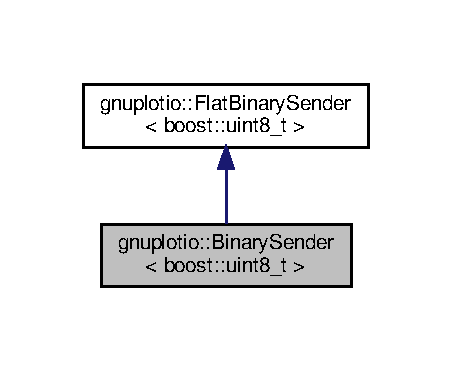
\includegraphics[width=217pt]{structgnuplotio_1_1BinarySender_3_01boost_1_1uint8__t_01_4__coll__graph}
\end{center}
\end{figure}
\subsection*{Additional Inherited Members}


The documentation for this struct was generated from the following file\+:\begin{DoxyCompactItemize}
\item 
include/gnuplot-\/iostream.\+h\end{DoxyCompactItemize}

\hypertarget{structgnuplotio_1_1BinarySender_3_01double_01_4}{}\section{gnuplotio\+:\+:Binary\+Sender$<$ double $>$ Struct Template Reference}
\label{structgnuplotio_1_1BinarySender_3_01double_01_4}\index{gnuplotio\+::\+Binary\+Sender$<$ double $>$@{gnuplotio\+::\+Binary\+Sender$<$ double $>$}}


Inheritance diagram for gnuplotio\+:\+:Binary\+Sender$<$ double $>$\+:\nopagebreak
\begin{figure}[H]
\begin{center}
\leavevmode
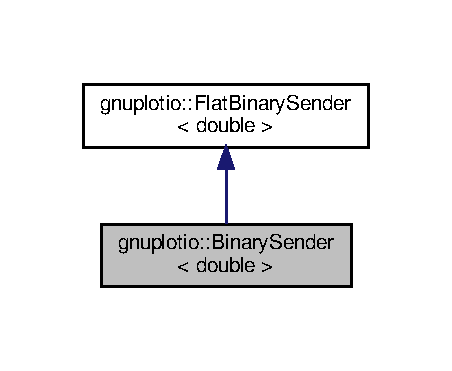
\includegraphics[width=217pt]{structgnuplotio_1_1BinarySender_3_01double_01_4__inherit__graph}
\end{center}
\end{figure}


Collaboration diagram for gnuplotio\+:\+:Binary\+Sender$<$ double $>$\+:\nopagebreak
\begin{figure}[H]
\begin{center}
\leavevmode
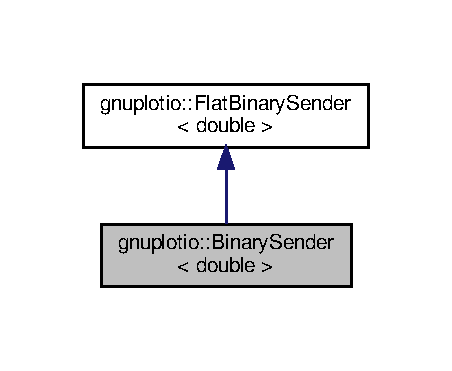
\includegraphics[width=217pt]{structgnuplotio_1_1BinarySender_3_01double_01_4__coll__graph}
\end{center}
\end{figure}
\subsection*{Additional Inherited Members}


The documentation for this struct was generated from the following file\+:\begin{DoxyCompactItemize}
\item 
include/gnuplot-\/iostream.\+h\end{DoxyCompactItemize}

\hypertarget{structgnuplotio_1_1BinarySender_3_01float_01_4}{}\section{gnuplotio\+:\+:Binary\+Sender$<$ float $>$ Struct Template Reference}
\label{structgnuplotio_1_1BinarySender_3_01float_01_4}\index{gnuplotio\+::\+Binary\+Sender$<$ float $>$@{gnuplotio\+::\+Binary\+Sender$<$ float $>$}}


Inheritance diagram for gnuplotio\+:\+:Binary\+Sender$<$ float $>$\+:\nopagebreak
\begin{figure}[H]
\begin{center}
\leavevmode
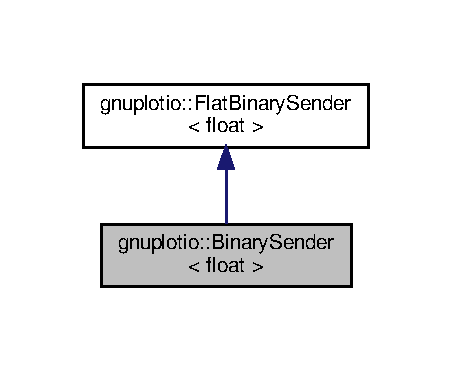
\includegraphics[width=217pt]{structgnuplotio_1_1BinarySender_3_01float_01_4__inherit__graph}
\end{center}
\end{figure}


Collaboration diagram for gnuplotio\+:\+:Binary\+Sender$<$ float $>$\+:\nopagebreak
\begin{figure}[H]
\begin{center}
\leavevmode
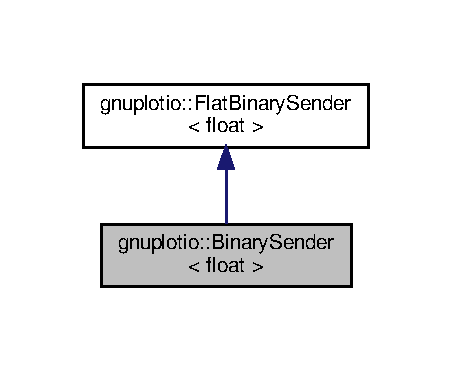
\includegraphics[width=217pt]{structgnuplotio_1_1BinarySender_3_01float_01_4__coll__graph}
\end{center}
\end{figure}
\subsection*{Additional Inherited Members}


The documentation for this struct was generated from the following file\+:\begin{DoxyCompactItemize}
\item 
include/gnuplot-\/iostream.\+h\end{DoxyCompactItemize}

\hypertarget{structgnuplotio_1_1BinarySender_3_01std_1_1complex_3_01T_01_4_01_4}{}\section{gnuplotio\+:\+:Binary\+Sender$<$ std\+:\+:complex$<$ T $>$ $>$ Struct Template Reference}
\label{structgnuplotio_1_1BinarySender_3_01std_1_1complex_3_01T_01_4_01_4}\index{gnuplotio\+::\+Binary\+Sender$<$ std\+::complex$<$ T $>$ $>$@{gnuplotio\+::\+Binary\+Sender$<$ std\+::complex$<$ T $>$ $>$}}
\subsection*{Static Public Member Functions}
\begin{DoxyCompactItemize}
\item 
\mbox{\Hypertarget{structgnuplotio_1_1BinarySender_3_01std_1_1complex_3_01T_01_4_01_4_a759de700a1cd68000830a4b15a6fec49}\label{structgnuplotio_1_1BinarySender_3_01std_1_1complex_3_01T_01_4_01_4_a759de700a1cd68000830a4b15a6fec49}} 
static void {\bfseries send} (std\+::ostream \&stream, const std\+::complex$<$ T $>$ \&v)
\end{DoxyCompactItemize}


The documentation for this struct was generated from the following file\+:\begin{DoxyCompactItemize}
\item 
include/gnuplot-\/iostream.\+h\end{DoxyCompactItemize}

\hypertarget{structgnuplotio_1_1BinarySender_3_01std_1_1pair_3_01T_00_01U_01_4_01_4}{}\section{gnuplotio\+:\+:Binary\+Sender$<$ std\+:\+:pair$<$ T, U $>$ $>$ Struct Template Reference}
\label{structgnuplotio_1_1BinarySender_3_01std_1_1pair_3_01T_00_01U_01_4_01_4}\index{gnuplotio\+::\+Binary\+Sender$<$ std\+::pair$<$ T, U $>$ $>$@{gnuplotio\+::\+Binary\+Sender$<$ std\+::pair$<$ T, U $>$ $>$}}
\subsection*{Static Public Member Functions}
\begin{DoxyCompactItemize}
\item 
\mbox{\Hypertarget{structgnuplotio_1_1BinarySender_3_01std_1_1pair_3_01T_00_01U_01_4_01_4_a9d949c8e7b1dea493288b0a2dd95cbff}\label{structgnuplotio_1_1BinarySender_3_01std_1_1pair_3_01T_00_01U_01_4_01_4_a9d949c8e7b1dea493288b0a2dd95cbff}} 
static void {\bfseries send} (std\+::ostream \&stream, const std\+::pair$<$ T, U $>$ \&v)
\end{DoxyCompactItemize}


The documentation for this struct was generated from the following file\+:\begin{DoxyCompactItemize}
\item 
include/gnuplot-\/iostream.\+h\end{DoxyCompactItemize}

\hypertarget{structgnuplotio_1_1BinarySender_3_01T_00_01typename_01boost_1_1enable__if_3_01boost_1_1mpl_1_1anab84516ea337555045555dbce2b6c996}{}\section{gnuplotio\+:\+:Binary\+Sender$<$ T, typename boost\+:\+:enable\+\_\+if$<$ boost\+:\+:mpl\+:\+:and\+\_\+$<$ is\+\_\+boost\+\_\+tuple$<$ T $>$, boost\+:\+:mpl\+:\+:not\+\_\+$<$ is\+\_\+boost\+\_\+tuple\+\_\+nulltype$<$ typename T\+:\+:tail\+\_\+type $>$ $>$ $>$ $>$\+:\+:type $>$ Struct Template Reference}
\label{structgnuplotio_1_1BinarySender_3_01T_00_01typename_01boost_1_1enable__if_3_01boost_1_1mpl_1_1anab84516ea337555045555dbce2b6c996}\index{gnuplotio\+::\+Binary\+Sender$<$ T, typename boost\+::enable\+\_\+if$<$ boost\+::mpl\+::and\+\_\+$<$ is\+\_\+boost\+\_\+tuple$<$ T $>$, boost\+::mpl\+::not\+\_\+$<$ is\+\_\+boost\+\_\+tuple\+\_\+nulltype$<$ typename T\+::tail\+\_\+type $>$ $>$ $>$ $>$\+::type $>$@{gnuplotio\+::\+Binary\+Sender$<$ T, typename boost\+::enable\+\_\+if$<$ boost\+::mpl\+::and\+\_\+$<$ is\+\_\+boost\+\_\+tuple$<$ T $>$, boost\+::mpl\+::not\+\_\+$<$ is\+\_\+boost\+\_\+tuple\+\_\+nulltype$<$ typename T\+::tail\+\_\+type $>$ $>$ $>$ $>$\+::type $>$}}
\subsection*{Static Public Member Functions}
\begin{DoxyCompactItemize}
\item 
\mbox{\Hypertarget{structgnuplotio_1_1BinarySender_3_01T_00_01typename_01boost_1_1enable__if_3_01boost_1_1mpl_1_1anab84516ea337555045555dbce2b6c996_a90bdbe9d299646a871882da19fdb30a9}\label{structgnuplotio_1_1BinarySender_3_01T_00_01typename_01boost_1_1enable__if_3_01boost_1_1mpl_1_1anab84516ea337555045555dbce2b6c996_a90bdbe9d299646a871882da19fdb30a9}} 
static void {\bfseries send} (std\+::ostream \&stream, const T \&v)
\end{DoxyCompactItemize}


The documentation for this struct was generated from the following file\+:\begin{DoxyCompactItemize}
\item 
include/gnuplot-\/iostream.\+h\end{DoxyCompactItemize}

\hypertarget{structgnuplotio_1_1BinarySender_3_01T_00_01typename_01boost_1_1enable__if_3_01boost_1_1mpl_1_1anbc7c19c30874558f14f1e5020da805a3}{}\section{gnuplotio\+:\+:Binary\+Sender$<$ T, typename boost\+:\+:enable\+\_\+if$<$ boost\+:\+:mpl\+:\+:and\+\_\+$<$ is\+\_\+boost\+\_\+tuple$<$ T $>$, is\+\_\+boost\+\_\+tuple\+\_\+nulltype$<$ typename T\+:\+:tail\+\_\+type $>$ $>$ $>$\+:\+:type $>$ Struct Template Reference}
\label{structgnuplotio_1_1BinarySender_3_01T_00_01typename_01boost_1_1enable__if_3_01boost_1_1mpl_1_1anbc7c19c30874558f14f1e5020da805a3}\index{gnuplotio\+::\+Binary\+Sender$<$ T, typename boost\+::enable\+\_\+if$<$ boost\+::mpl\+::and\+\_\+$<$ is\+\_\+boost\+\_\+tuple$<$ T $>$, is\+\_\+boost\+\_\+tuple\+\_\+nulltype$<$ typename T\+::tail\+\_\+type $>$ $>$ $>$\+::type $>$@{gnuplotio\+::\+Binary\+Sender$<$ T, typename boost\+::enable\+\_\+if$<$ boost\+::mpl\+::and\+\_\+$<$ is\+\_\+boost\+\_\+tuple$<$ T $>$, is\+\_\+boost\+\_\+tuple\+\_\+nulltype$<$ typename T\+::tail\+\_\+type $>$ $>$ $>$\+::type $>$}}
\subsection*{Static Public Member Functions}
\begin{DoxyCompactItemize}
\item 
\mbox{\Hypertarget{structgnuplotio_1_1BinarySender_3_01T_00_01typename_01boost_1_1enable__if_3_01boost_1_1mpl_1_1anbc7c19c30874558f14f1e5020da805a3_a50e54b7f2aba37f1f9e63fa81941b6d6}\label{structgnuplotio_1_1BinarySender_3_01T_00_01typename_01boost_1_1enable__if_3_01boost_1_1mpl_1_1anbc7c19c30874558f14f1e5020da805a3_a50e54b7f2aba37f1f9e63fa81941b6d6}} 
static void {\bfseries send} (std\+::ostream \&stream, const T \&v)
\end{DoxyCompactItemize}


The documentation for this struct was generated from the following file\+:\begin{DoxyCompactItemize}
\item 
include/gnuplot-\/iostream.\+h\end{DoxyCompactItemize}

\hypertarget{structgnuplotio_1_1BinfmtSender}{}\section{gnuplotio\+:\+:Binfmt\+Sender$<$ T, Enable $>$ Struct Template Reference}
\label{structgnuplotio_1_1BinfmtSender}\index{gnuplotio\+::\+Binfmt\+Sender$<$ T, Enable $>$@{gnuplotio\+::\+Binfmt\+Sender$<$ T, Enable $>$}}
\subsection*{Public Member Functions}
\begin{DoxyCompactItemize}
\item 
\mbox{\Hypertarget{structgnuplotio_1_1BinfmtSender_a02d7d348067625dc099e27249c24780a}\label{structgnuplotio_1_1BinfmtSender_a02d7d348067625dc099e27249c24780a}} 
{\bfseries G\+N\+U\+P\+L\+O\+T\+\_\+\+S\+T\+A\+T\+I\+C\+\_\+\+A\+S\+S\+E\+R\+T\+\_\+\+M\+SG} ((sizeof(T)==0), \char`\"{}Binfmt\+Sender class not specialized for this type\char`\"{})
\end{DoxyCompactItemize}
\subsection*{Static Public Member Functions}
\begin{DoxyCompactItemize}
\item 
\mbox{\Hypertarget{structgnuplotio_1_1BinfmtSender_a762010e3172c02e981252f93185b29c8}\label{structgnuplotio_1_1BinfmtSender_a762010e3172c02e981252f93185b29c8}} 
static void {\bfseries send} (std\+::ostream \&)
\end{DoxyCompactItemize}


The documentation for this struct was generated from the following file\+:\begin{DoxyCompactItemize}
\item 
include/gnuplot-\/iostream.\+h\end{DoxyCompactItemize}

\hypertarget{structgnuplotio_1_1BinfmtSender_3_01boost_1_1int16__t_01_4}{}\section{gnuplotio\+:\+:Binfmt\+Sender$<$ boost\+:\+:int16\+\_\+t $>$ Struct Template Reference}
\label{structgnuplotio_1_1BinfmtSender_3_01boost_1_1int16__t_01_4}\index{gnuplotio\+::\+Binfmt\+Sender$<$ boost\+::int16\+\_\+t $>$@{gnuplotio\+::\+Binfmt\+Sender$<$ boost\+::int16\+\_\+t $>$}}
\subsection*{Static Public Member Functions}
\begin{DoxyCompactItemize}
\item 
\mbox{\Hypertarget{structgnuplotio_1_1BinfmtSender_3_01boost_1_1int16__t_01_4_a6d3c1b829c9196fa9d1f53bd78a90e34}\label{structgnuplotio_1_1BinfmtSender_3_01boost_1_1int16__t_01_4_a6d3c1b829c9196fa9d1f53bd78a90e34}} 
static void {\bfseries send} (std\+::ostream \&stream)
\end{DoxyCompactItemize}


The documentation for this struct was generated from the following file\+:\begin{DoxyCompactItemize}
\item 
include/gnuplot-\/iostream.\+h\end{DoxyCompactItemize}

\hypertarget{structgnuplotio_1_1BinfmtSender_3_01boost_1_1int32__t_01_4}{}\section{gnuplotio\+:\+:Binfmt\+Sender$<$ boost\+:\+:int32\+\_\+t $>$ Struct Template Reference}
\label{structgnuplotio_1_1BinfmtSender_3_01boost_1_1int32__t_01_4}\index{gnuplotio\+::\+Binfmt\+Sender$<$ boost\+::int32\+\_\+t $>$@{gnuplotio\+::\+Binfmt\+Sender$<$ boost\+::int32\+\_\+t $>$}}
\subsection*{Static Public Member Functions}
\begin{DoxyCompactItemize}
\item 
\mbox{\Hypertarget{structgnuplotio_1_1BinfmtSender_3_01boost_1_1int32__t_01_4_a44f75b80ef3f5def62eaa2093810fd35}\label{structgnuplotio_1_1BinfmtSender_3_01boost_1_1int32__t_01_4_a44f75b80ef3f5def62eaa2093810fd35}} 
static void {\bfseries send} (std\+::ostream \&stream)
\end{DoxyCompactItemize}


The documentation for this struct was generated from the following file\+:\begin{DoxyCompactItemize}
\item 
include/gnuplot-\/iostream.\+h\end{DoxyCompactItemize}

\hypertarget{structgnuplotio_1_1BinfmtSender_3_01boost_1_1int64__t_01_4}{}\section{gnuplotio\+:\+:Binfmt\+Sender$<$ boost\+:\+:int64\+\_\+t $>$ Struct Template Reference}
\label{structgnuplotio_1_1BinfmtSender_3_01boost_1_1int64__t_01_4}\index{gnuplotio\+::\+Binfmt\+Sender$<$ boost\+::int64\+\_\+t $>$@{gnuplotio\+::\+Binfmt\+Sender$<$ boost\+::int64\+\_\+t $>$}}
\subsection*{Static Public Member Functions}
\begin{DoxyCompactItemize}
\item 
\mbox{\Hypertarget{structgnuplotio_1_1BinfmtSender_3_01boost_1_1int64__t_01_4_a57423f02a4526e15d7d821606b1c8c81}\label{structgnuplotio_1_1BinfmtSender_3_01boost_1_1int64__t_01_4_a57423f02a4526e15d7d821606b1c8c81}} 
static void {\bfseries send} (std\+::ostream \&stream)
\end{DoxyCompactItemize}


The documentation for this struct was generated from the following file\+:\begin{DoxyCompactItemize}
\item 
include/gnuplot-\/iostream.\+h\end{DoxyCompactItemize}

\hypertarget{structgnuplotio_1_1BinfmtSender_3_01boost_1_1int8__t_01_4}{}\section{gnuplotio\+:\+:Binfmt\+Sender$<$ boost\+:\+:int8\+\_\+t $>$ Struct Template Reference}
\label{structgnuplotio_1_1BinfmtSender_3_01boost_1_1int8__t_01_4}\index{gnuplotio\+::\+Binfmt\+Sender$<$ boost\+::int8\+\_\+t $>$@{gnuplotio\+::\+Binfmt\+Sender$<$ boost\+::int8\+\_\+t $>$}}
\subsection*{Static Public Member Functions}
\begin{DoxyCompactItemize}
\item 
\mbox{\Hypertarget{structgnuplotio_1_1BinfmtSender_3_01boost_1_1int8__t_01_4_a6f61d43b0da25f044bfad0d45fe888b4}\label{structgnuplotio_1_1BinfmtSender_3_01boost_1_1int8__t_01_4_a6f61d43b0da25f044bfad0d45fe888b4}} 
static void {\bfseries send} (std\+::ostream \&stream)
\end{DoxyCompactItemize}


The documentation for this struct was generated from the following file\+:\begin{DoxyCompactItemize}
\item 
include/gnuplot-\/iostream.\+h\end{DoxyCompactItemize}

\hypertarget{structgnuplotio_1_1BinfmtSender_3_01boost_1_1uint16__t_01_4}{}\section{gnuplotio\+:\+:Binfmt\+Sender$<$ boost\+:\+:uint16\+\_\+t $>$ Struct Template Reference}
\label{structgnuplotio_1_1BinfmtSender_3_01boost_1_1uint16__t_01_4}\index{gnuplotio\+::\+Binfmt\+Sender$<$ boost\+::uint16\+\_\+t $>$@{gnuplotio\+::\+Binfmt\+Sender$<$ boost\+::uint16\+\_\+t $>$}}
\subsection*{Static Public Member Functions}
\begin{DoxyCompactItemize}
\item 
\mbox{\Hypertarget{structgnuplotio_1_1BinfmtSender_3_01boost_1_1uint16__t_01_4_a7bb7f0a62a21496b9e85ce35f0170717}\label{structgnuplotio_1_1BinfmtSender_3_01boost_1_1uint16__t_01_4_a7bb7f0a62a21496b9e85ce35f0170717}} 
static void {\bfseries send} (std\+::ostream \&stream)
\end{DoxyCompactItemize}


The documentation for this struct was generated from the following file\+:\begin{DoxyCompactItemize}
\item 
include/gnuplot-\/iostream.\+h\end{DoxyCompactItemize}

\hypertarget{structgnuplotio_1_1BinfmtSender_3_01boost_1_1uint32__t_01_4}{}\section{gnuplotio\+:\+:Binfmt\+Sender$<$ boost\+:\+:uint32\+\_\+t $>$ Struct Template Reference}
\label{structgnuplotio_1_1BinfmtSender_3_01boost_1_1uint32__t_01_4}\index{gnuplotio\+::\+Binfmt\+Sender$<$ boost\+::uint32\+\_\+t $>$@{gnuplotio\+::\+Binfmt\+Sender$<$ boost\+::uint32\+\_\+t $>$}}
\subsection*{Static Public Member Functions}
\begin{DoxyCompactItemize}
\item 
\mbox{\Hypertarget{structgnuplotio_1_1BinfmtSender_3_01boost_1_1uint32__t_01_4_a134bce57dc5bb3e06c1b369a9826403b}\label{structgnuplotio_1_1BinfmtSender_3_01boost_1_1uint32__t_01_4_a134bce57dc5bb3e06c1b369a9826403b}} 
static void {\bfseries send} (std\+::ostream \&stream)
\end{DoxyCompactItemize}


The documentation for this struct was generated from the following file\+:\begin{DoxyCompactItemize}
\item 
include/gnuplot-\/iostream.\+h\end{DoxyCompactItemize}

\hypertarget{structgnuplotio_1_1BinfmtSender_3_01boost_1_1uint64__t_01_4}{}\section{gnuplotio\+:\+:Binfmt\+Sender$<$ boost\+:\+:uint64\+\_\+t $>$ Struct Template Reference}
\label{structgnuplotio_1_1BinfmtSender_3_01boost_1_1uint64__t_01_4}\index{gnuplotio\+::\+Binfmt\+Sender$<$ boost\+::uint64\+\_\+t $>$@{gnuplotio\+::\+Binfmt\+Sender$<$ boost\+::uint64\+\_\+t $>$}}
\subsection*{Static Public Member Functions}
\begin{DoxyCompactItemize}
\item 
\mbox{\Hypertarget{structgnuplotio_1_1BinfmtSender_3_01boost_1_1uint64__t_01_4_a9f57162a6baf940675236235556f62ba}\label{structgnuplotio_1_1BinfmtSender_3_01boost_1_1uint64__t_01_4_a9f57162a6baf940675236235556f62ba}} 
static void {\bfseries send} (std\+::ostream \&stream)
\end{DoxyCompactItemize}


The documentation for this struct was generated from the following file\+:\begin{DoxyCompactItemize}
\item 
include/gnuplot-\/iostream.\+h\end{DoxyCompactItemize}

\hypertarget{structgnuplotio_1_1BinfmtSender_3_01boost_1_1uint8__t_01_4}{}\section{gnuplotio\+:\+:Binfmt\+Sender$<$ boost\+:\+:uint8\+\_\+t $>$ Struct Template Reference}
\label{structgnuplotio_1_1BinfmtSender_3_01boost_1_1uint8__t_01_4}\index{gnuplotio\+::\+Binfmt\+Sender$<$ boost\+::uint8\+\_\+t $>$@{gnuplotio\+::\+Binfmt\+Sender$<$ boost\+::uint8\+\_\+t $>$}}
\subsection*{Static Public Member Functions}
\begin{DoxyCompactItemize}
\item 
\mbox{\Hypertarget{structgnuplotio_1_1BinfmtSender_3_01boost_1_1uint8__t_01_4_a57d45c45f1ee19614c972bc82c4b214c}\label{structgnuplotio_1_1BinfmtSender_3_01boost_1_1uint8__t_01_4_a57d45c45f1ee19614c972bc82c4b214c}} 
static void {\bfseries send} (std\+::ostream \&stream)
\end{DoxyCompactItemize}


The documentation for this struct was generated from the following file\+:\begin{DoxyCompactItemize}
\item 
include/gnuplot-\/iostream.\+h\end{DoxyCompactItemize}

\hypertarget{structgnuplotio_1_1BinfmtSender_3_01double_01_4}{}\section{gnuplotio\+:\+:Binfmt\+Sender$<$ double $>$ Struct Template Reference}
\label{structgnuplotio_1_1BinfmtSender_3_01double_01_4}\index{gnuplotio\+::\+Binfmt\+Sender$<$ double $>$@{gnuplotio\+::\+Binfmt\+Sender$<$ double $>$}}
\subsection*{Static Public Member Functions}
\begin{DoxyCompactItemize}
\item 
\mbox{\Hypertarget{structgnuplotio_1_1BinfmtSender_3_01double_01_4_a455b75492a6a86398374d14a2bfc7238}\label{structgnuplotio_1_1BinfmtSender_3_01double_01_4_a455b75492a6a86398374d14a2bfc7238}} 
static void {\bfseries send} (std\+::ostream \&stream)
\end{DoxyCompactItemize}


The documentation for this struct was generated from the following file\+:\begin{DoxyCompactItemize}
\item 
include/gnuplot-\/iostream.\+h\end{DoxyCompactItemize}

\hypertarget{structgnuplotio_1_1BinfmtSender_3_01float_01_4}{}\section{gnuplotio\+:\+:Binfmt\+Sender$<$ float $>$ Struct Template Reference}
\label{structgnuplotio_1_1BinfmtSender_3_01float_01_4}\index{gnuplotio\+::\+Binfmt\+Sender$<$ float $>$@{gnuplotio\+::\+Binfmt\+Sender$<$ float $>$}}
\subsection*{Static Public Member Functions}
\begin{DoxyCompactItemize}
\item 
\mbox{\Hypertarget{structgnuplotio_1_1BinfmtSender_3_01float_01_4_ae9c6a1915ee24e54ea5ed1a22c54fee1}\label{structgnuplotio_1_1BinfmtSender_3_01float_01_4_ae9c6a1915ee24e54ea5ed1a22c54fee1}} 
static void {\bfseries send} (std\+::ostream \&stream)
\end{DoxyCompactItemize}


The documentation for this struct was generated from the following file\+:\begin{DoxyCompactItemize}
\item 
include/gnuplot-\/iostream.\+h\end{DoxyCompactItemize}

\hypertarget{structgnuplotio_1_1BinfmtSender_3_01std_1_1complex_3_01T_01_4_01_4}{}\section{gnuplotio\+:\+:Binfmt\+Sender$<$ std\+:\+:complex$<$ T $>$ $>$ Struct Template Reference}
\label{structgnuplotio_1_1BinfmtSender_3_01std_1_1complex_3_01T_01_4_01_4}\index{gnuplotio\+::\+Binfmt\+Sender$<$ std\+::complex$<$ T $>$ $>$@{gnuplotio\+::\+Binfmt\+Sender$<$ std\+::complex$<$ T $>$ $>$}}
\subsection*{Static Public Member Functions}
\begin{DoxyCompactItemize}
\item 
\mbox{\Hypertarget{structgnuplotio_1_1BinfmtSender_3_01std_1_1complex_3_01T_01_4_01_4_a64633d068c93ef2822ee3aa6ef39d623}\label{structgnuplotio_1_1BinfmtSender_3_01std_1_1complex_3_01T_01_4_01_4_a64633d068c93ef2822ee3aa6ef39d623}} 
static void {\bfseries send} (std\+::ostream \&stream)
\end{DoxyCompactItemize}


The documentation for this struct was generated from the following file\+:\begin{DoxyCompactItemize}
\item 
include/gnuplot-\/iostream.\+h\end{DoxyCompactItemize}

\hypertarget{structgnuplotio_1_1BinfmtSender_3_01std_1_1pair_3_01T_00_01U_01_4_01_4}{}\section{gnuplotio\+:\+:Binfmt\+Sender$<$ std\+:\+:pair$<$ T, U $>$ $>$ Struct Template Reference}
\label{structgnuplotio_1_1BinfmtSender_3_01std_1_1pair_3_01T_00_01U_01_4_01_4}\index{gnuplotio\+::\+Binfmt\+Sender$<$ std\+::pair$<$ T, U $>$ $>$@{gnuplotio\+::\+Binfmt\+Sender$<$ std\+::pair$<$ T, U $>$ $>$}}
\subsection*{Static Public Member Functions}
\begin{DoxyCompactItemize}
\item 
\mbox{\Hypertarget{structgnuplotio_1_1BinfmtSender_3_01std_1_1pair_3_01T_00_01U_01_4_01_4_a08b2bedbc54824cd202c664116e37243}\label{structgnuplotio_1_1BinfmtSender_3_01std_1_1pair_3_01T_00_01U_01_4_01_4_a08b2bedbc54824cd202c664116e37243}} 
static void {\bfseries send} (std\+::ostream \&stream)
\end{DoxyCompactItemize}


The documentation for this struct was generated from the following file\+:\begin{DoxyCompactItemize}
\item 
include/gnuplot-\/iostream.\+h\end{DoxyCompactItemize}

\hypertarget{structgnuplotio_1_1BinfmtSender_3_01T_00_01typename_01boost_1_1enable__if_3_01boost_1_1mpl_1_1an42b95f03faee3ff44b47c946e1ea6e52}{}\section{gnuplotio\+:\+:Binfmt\+Sender$<$ T, typename boost\+:\+:enable\+\_\+if$<$ boost\+:\+:mpl\+:\+:and\+\_\+$<$ is\+\_\+boost\+\_\+tuple$<$ T $>$, boost\+:\+:mpl\+:\+:not\+\_\+$<$ is\+\_\+boost\+\_\+tuple\+\_\+nulltype$<$ typename T\+:\+:tail\+\_\+type $>$ $>$ $>$ $>$\+:\+:type $>$ Struct Template Reference}
\label{structgnuplotio_1_1BinfmtSender_3_01T_00_01typename_01boost_1_1enable__if_3_01boost_1_1mpl_1_1an42b95f03faee3ff44b47c946e1ea6e52}\index{gnuplotio\+::\+Binfmt\+Sender$<$ T, typename boost\+::enable\+\_\+if$<$ boost\+::mpl\+::and\+\_\+$<$ is\+\_\+boost\+\_\+tuple$<$ T $>$, boost\+::mpl\+::not\+\_\+$<$ is\+\_\+boost\+\_\+tuple\+\_\+nulltype$<$ typename T\+::tail\+\_\+type $>$ $>$ $>$ $>$\+::type $>$@{gnuplotio\+::\+Binfmt\+Sender$<$ T, typename boost\+::enable\+\_\+if$<$ boost\+::mpl\+::and\+\_\+$<$ is\+\_\+boost\+\_\+tuple$<$ T $>$, boost\+::mpl\+::not\+\_\+$<$ is\+\_\+boost\+\_\+tuple\+\_\+nulltype$<$ typename T\+::tail\+\_\+type $>$ $>$ $>$ $>$\+::type $>$}}
\subsection*{Static Public Member Functions}
\begin{DoxyCompactItemize}
\item 
\mbox{\Hypertarget{structgnuplotio_1_1BinfmtSender_3_01T_00_01typename_01boost_1_1enable__if_3_01boost_1_1mpl_1_1an42b95f03faee3ff44b47c946e1ea6e52_a12e1b40a6ae29940661b7609df3c40ba}\label{structgnuplotio_1_1BinfmtSender_3_01T_00_01typename_01boost_1_1enable__if_3_01boost_1_1mpl_1_1an42b95f03faee3ff44b47c946e1ea6e52_a12e1b40a6ae29940661b7609df3c40ba}} 
static void {\bfseries send} (std\+::ostream \&stream)
\end{DoxyCompactItemize}


The documentation for this struct was generated from the following file\+:\begin{DoxyCompactItemize}
\item 
include/gnuplot-\/iostream.\+h\end{DoxyCompactItemize}

\hypertarget{structgnuplotio_1_1BinfmtSender_3_01T_00_01typename_01boost_1_1enable__if_3_01boost_1_1mpl_1_1an36b5089f0cb57748545b30004479b7ea}{}\section{gnuplotio\+:\+:Binfmt\+Sender$<$ T, typename boost\+:\+:enable\+\_\+if$<$ boost\+:\+:mpl\+:\+:and\+\_\+$<$ is\+\_\+boost\+\_\+tuple$<$ T $>$, is\+\_\+boost\+\_\+tuple\+\_\+nulltype$<$ typename T\+:\+:tail\+\_\+type $>$ $>$ $>$\+:\+:type $>$ Struct Template Reference}
\label{structgnuplotio_1_1BinfmtSender_3_01T_00_01typename_01boost_1_1enable__if_3_01boost_1_1mpl_1_1an36b5089f0cb57748545b30004479b7ea}\index{gnuplotio\+::\+Binfmt\+Sender$<$ T, typename boost\+::enable\+\_\+if$<$ boost\+::mpl\+::and\+\_\+$<$ is\+\_\+boost\+\_\+tuple$<$ T $>$, is\+\_\+boost\+\_\+tuple\+\_\+nulltype$<$ typename T\+::tail\+\_\+type $>$ $>$ $>$\+::type $>$@{gnuplotio\+::\+Binfmt\+Sender$<$ T, typename boost\+::enable\+\_\+if$<$ boost\+::mpl\+::and\+\_\+$<$ is\+\_\+boost\+\_\+tuple$<$ T $>$, is\+\_\+boost\+\_\+tuple\+\_\+nulltype$<$ typename T\+::tail\+\_\+type $>$ $>$ $>$\+::type $>$}}
\subsection*{Static Public Member Functions}
\begin{DoxyCompactItemize}
\item 
\mbox{\Hypertarget{structgnuplotio_1_1BinfmtSender_3_01T_00_01typename_01boost_1_1enable__if_3_01boost_1_1mpl_1_1an36b5089f0cb57748545b30004479b7ea_aa1850ae529cdb36fedc67c5ebfa3f871}\label{structgnuplotio_1_1BinfmtSender_3_01T_00_01typename_01boost_1_1enable__if_3_01boost_1_1mpl_1_1an36b5089f0cb57748545b30004479b7ea_aa1850ae529cdb36fedc67c5ebfa3f871}} 
static void {\bfseries send} (std\+::ostream \&stream)
\end{DoxyCompactItemize}


The documentation for this struct was generated from the following file\+:\begin{DoxyCompactItemize}
\item 
include/gnuplot-\/iostream.\+h\end{DoxyCompactItemize}

\hypertarget{structgnuplotio_1_1CastIntTextSender}{}\section{gnuplotio\+:\+:Cast\+Int\+Text\+Sender$<$ T $>$ Struct Template Reference}
\label{structgnuplotio_1_1CastIntTextSender}\index{gnuplotio\+::\+Cast\+Int\+Text\+Sender$<$ T $>$@{gnuplotio\+::\+Cast\+Int\+Text\+Sender$<$ T $>$}}
\subsection*{Static Public Member Functions}
\begin{DoxyCompactItemize}
\item 
\mbox{\Hypertarget{structgnuplotio_1_1CastIntTextSender_a42733f83f843a375437e7e5f716ea65e}\label{structgnuplotio_1_1CastIntTextSender_a42733f83f843a375437e7e5f716ea65e}} 
static void {\bfseries send} (std\+::ostream \&stream, const T \&v)
\end{DoxyCompactItemize}


The documentation for this struct was generated from the following file\+:\begin{DoxyCompactItemize}
\item 
include/gnuplot-\/iostream.\+h\end{DoxyCompactItemize}

\hypertarget{structgnuplotio_1_1ColUnwrapNo}{}\section{gnuplotio\+:\+:Col\+Unwrap\+No Struct Reference}
\label{structgnuplotio_1_1ColUnwrapNo}\index{gnuplotio\+::\+Col\+Unwrap\+No@{gnuplotio\+::\+Col\+Unwrap\+No}}


The documentation for this struct was generated from the following file\+:\begin{DoxyCompactItemize}
\item 
include/gnuplot-\/iostream.\+h\end{DoxyCompactItemize}

\hypertarget{structgnuplotio_1_1ColUnwrapYes}{}\section{gnuplotio\+:\+:Col\+Unwrap\+Yes Struct Reference}
\label{structgnuplotio_1_1ColUnwrapYes}\index{gnuplotio\+::\+Col\+Unwrap\+Yes@{gnuplotio\+::\+Col\+Unwrap\+Yes}}


The documentation for this struct was generated from the following file\+:\begin{DoxyCompactItemize}
\item 
include/gnuplot-\/iostream.\+h\end{DoxyCompactItemize}

\hypertarget{structgnuplotio_1_1dont__treat__as__stl__container}{}\section{gnuplotio\+:\+:dont\+\_\+treat\+\_\+as\+\_\+stl\+\_\+container$<$ T $>$ Struct Template Reference}
\label{structgnuplotio_1_1dont__treat__as__stl__container}\index{gnuplotio\+::dont\+\_\+treat\+\_\+as\+\_\+stl\+\_\+container$<$ T $>$@{gnuplotio\+::dont\+\_\+treat\+\_\+as\+\_\+stl\+\_\+container$<$ T $>$}}
\subsection*{Public Types}
\begin{DoxyCompactItemize}
\item 
\mbox{\Hypertarget{structgnuplotio_1_1dont__treat__as__stl__container_aa4404164a7547142376a9140ef07fd2a}\label{structgnuplotio_1_1dont__treat__as__stl__container_aa4404164a7547142376a9140ef07fd2a}} 
typedef boost\+::mpl\+::bool\+\_\+$<$ false $>$ {\bfseries type}
\end{DoxyCompactItemize}


The documentation for this struct was generated from the following file\+:\begin{DoxyCompactItemize}
\item 
include/gnuplot-\/iostream.\+h\end{DoxyCompactItemize}

\hypertarget{structgnuplotio_1_1Error__InappropriateDeref}{}\section{gnuplotio\+:\+:Error\+\_\+\+Inappropriate\+Deref Struct Reference}
\label{structgnuplotio_1_1Error__InappropriateDeref}\index{gnuplotio\+::\+Error\+\_\+\+Inappropriate\+Deref@{gnuplotio\+::\+Error\+\_\+\+Inappropriate\+Deref}}


The documentation for this struct was generated from the following file\+:\begin{DoxyCompactItemize}
\item 
include/gnuplot-\/iostream.\+h\end{DoxyCompactItemize}

\hypertarget{structgnuplotio_1_1Error__WasNotContainer}{}\section{gnuplotio\+:\+:Error\+\_\+\+Was\+Not\+Container Struct Reference}
\label{structgnuplotio_1_1Error__WasNotContainer}\index{gnuplotio\+::\+Error\+\_\+\+Was\+Not\+Container@{gnuplotio\+::\+Error\+\_\+\+Was\+Not\+Container}}
\subsection*{Public Types}
\begin{DoxyCompactItemize}
\item 
\mbox{\Hypertarget{structgnuplotio_1_1Error__WasNotContainer_aeac5de90c903be765130fc14f85dfb00}\label{structgnuplotio_1_1Error__WasNotContainer_aeac5de90c903be765130fc14f85dfb00}} 
typedef void {\bfseries subiter\+\_\+type}
\end{DoxyCompactItemize}


The documentation for this struct was generated from the following file\+:\begin{DoxyCompactItemize}
\item 
include/gnuplot-\/iostream.\+h\end{DoxyCompactItemize}

\hypertarget{structgnuplotio_1_1FileHandleWrapper}{}\section{gnuplotio\+:\+:File\+Handle\+Wrapper Struct Reference}
\label{structgnuplotio_1_1FileHandleWrapper}\index{gnuplotio\+::\+File\+Handle\+Wrapper@{gnuplotio\+::\+File\+Handle\+Wrapper}}


Inheritance diagram for gnuplotio\+:\+:File\+Handle\+Wrapper\+:\nopagebreak
\begin{figure}[H]
\begin{center}
\leavevmode
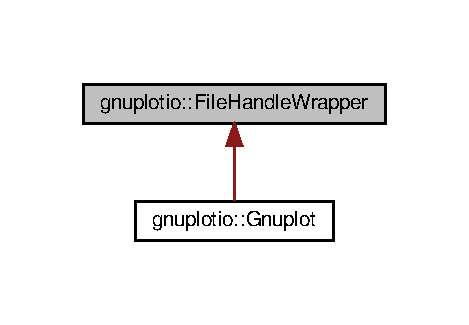
\includegraphics[width=225pt]{structgnuplotio_1_1FileHandleWrapper__inherit__graph}
\end{center}
\end{figure}
\subsection*{Public Member Functions}
\begin{DoxyCompactItemize}
\item 
\mbox{\Hypertarget{structgnuplotio_1_1FileHandleWrapper_a26b2378e193a9c41be5aed97e11f9411}\label{structgnuplotio_1_1FileHandleWrapper_a26b2378e193a9c41be5aed97e11f9411}} 
{\bfseries File\+Handle\+Wrapper} (std\+::\+F\+I\+LE $\ast$\+\_\+fh, bool \+\_\+should\+\_\+use\+\_\+pclose)
\item 
\mbox{\Hypertarget{structgnuplotio_1_1FileHandleWrapper_acafac45efd9c78ce621af4f3228c6f67}\label{structgnuplotio_1_1FileHandleWrapper_acafac45efd9c78ce621af4f3228c6f67}} 
void {\bfseries fh\+\_\+close} ()
\item 
\mbox{\Hypertarget{structgnuplotio_1_1FileHandleWrapper_a3202ccd15d624f26dd2cf699d3456de6}\label{structgnuplotio_1_1FileHandleWrapper_a3202ccd15d624f26dd2cf699d3456de6}} 
int {\bfseries fh\+\_\+fileno} ()
\end{DoxyCompactItemize}
\subsection*{Public Attributes}
\begin{DoxyCompactItemize}
\item 
\mbox{\Hypertarget{structgnuplotio_1_1FileHandleWrapper_adcb58bfcd9dbdba000a7e7395bee2ef9}\label{structgnuplotio_1_1FileHandleWrapper_adcb58bfcd9dbdba000a7e7395bee2ef9}} 
std\+::\+F\+I\+LE $\ast$ {\bfseries wrapped\+\_\+fh}
\item 
\mbox{\Hypertarget{structgnuplotio_1_1FileHandleWrapper_a11b63ed64cf53167e26c5273778d90ea}\label{structgnuplotio_1_1FileHandleWrapper_a11b63ed64cf53167e26c5273778d90ea}} 
bool {\bfseries should\+\_\+use\+\_\+pclose}
\end{DoxyCompactItemize}


The documentation for this struct was generated from the following file\+:\begin{DoxyCompactItemize}
\item 
include/gnuplot-\/iostream.\+h\end{DoxyCompactItemize}

\hypertarget{structgnuplotio_1_1FlatBinarySender}{}\section{gnuplotio\+:\+:Flat\+Binary\+Sender$<$ T $>$ Struct Template Reference}
\label{structgnuplotio_1_1FlatBinarySender}\index{gnuplotio\+::\+Flat\+Binary\+Sender$<$ T $>$@{gnuplotio\+::\+Flat\+Binary\+Sender$<$ T $>$}}
\subsection*{Static Public Member Functions}
\begin{DoxyCompactItemize}
\item 
\mbox{\Hypertarget{structgnuplotio_1_1FlatBinarySender_a24d085492f2539c14033cd5c6ba75ba5}\label{structgnuplotio_1_1FlatBinarySender_a24d085492f2539c14033cd5c6ba75ba5}} 
static void {\bfseries send} (std\+::ostream \&stream, const T \&v)
\end{DoxyCompactItemize}


The documentation for this struct was generated from the following file\+:\begin{DoxyCompactItemize}
\item 
include/gnuplot-\/iostream.\+h\end{DoxyCompactItemize}

\hypertarget{structgnuplotio_1_1FloatTextSender}{}\section{gnuplotio\+:\+:Float\+Text\+Sender$<$ T $>$ Struct Template Reference}
\label{structgnuplotio_1_1FloatTextSender}\index{gnuplotio\+::\+Float\+Text\+Sender$<$ T $>$@{gnuplotio\+::\+Float\+Text\+Sender$<$ T $>$}}
\subsection*{Static Public Member Functions}
\begin{DoxyCompactItemize}
\item 
\mbox{\Hypertarget{structgnuplotio_1_1FloatTextSender_aed6b6c3a95b1396688800d6d1f2fc299}\label{structgnuplotio_1_1FloatTextSender_aed6b6c3a95b1396688800d6d1f2fc299}} 
static void {\bfseries send} (std\+::ostream \&stream, const T \&v)
\end{DoxyCompactItemize}


The documentation for this struct was generated from the following file\+:\begin{DoxyCompactItemize}
\item 
include/gnuplot-\/iostream.\+h\end{DoxyCompactItemize}

\hypertarget{classgnuplotio_1_1Gnuplot}{}\section{gnuplotio\+:\+:Gnuplot Class Reference}
\label{classgnuplotio_1_1Gnuplot}\index{gnuplotio\+::\+Gnuplot@{gnuplotio\+::\+Gnuplot}}


Inheritance diagram for gnuplotio\+:\+:Gnuplot\+:\nopagebreak
\begin{figure}[H]
\begin{center}
\leavevmode
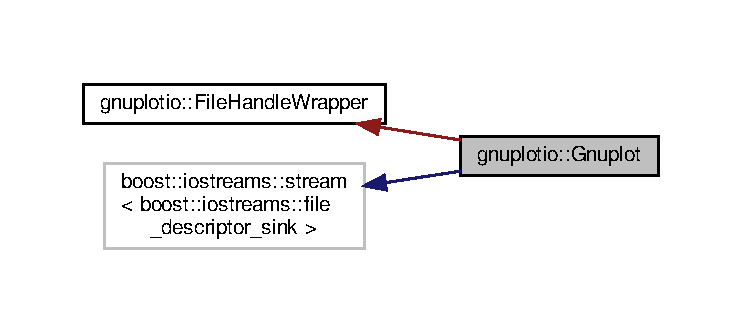
\includegraphics[width=350pt]{classgnuplotio_1_1Gnuplot__inherit__graph}
\end{center}
\end{figure}


Collaboration diagram for gnuplotio\+:\+:Gnuplot\+:\nopagebreak
\begin{figure}[H]
\begin{center}
\leavevmode
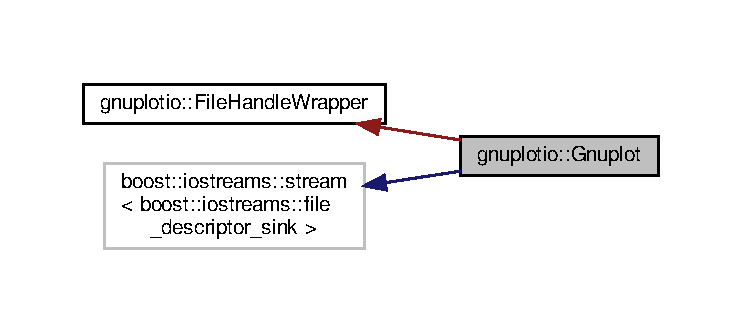
\includegraphics[width=350pt]{classgnuplotio_1_1Gnuplot__coll__graph}
\end{center}
\end{figure}
\subsection*{Public Member Functions}
\begin{DoxyCompactItemize}
\item 
\mbox{\Hypertarget{classgnuplotio_1_1Gnuplot_ab2fb14389ab63ad5d9b2e57169bbbf1d}\label{classgnuplotio_1_1Gnuplot_ab2fb14389ab63ad5d9b2e57169bbbf1d}} 
{\bfseries Gnuplot} (const std\+::string \&\+\_\+cmd=\char`\"{}\char`\"{})
\item 
\mbox{\Hypertarget{classgnuplotio_1_1Gnuplot_a4a4f48a548e6ce6d485ca0a868410078}\label{classgnuplotio_1_1Gnuplot_a4a4f48a548e6ce6d485ca0a868410078}} 
{\bfseries Gnuplot} (F\+I\+LE $\ast$\+\_\+fh)
\item 
\mbox{\Hypertarget{classgnuplotio_1_1Gnuplot_a0d62f80988c3db4413a668e366406393}\label{classgnuplotio_1_1Gnuplot_a0d62f80988c3db4413a668e366406393}} 
void {\bfseries clear\+Tmpfiles} ()
\item 
\mbox{\Hypertarget{classgnuplotio_1_1Gnuplot_ae3f4c07960aa5601cc72158be67f945c}\label{classgnuplotio_1_1Gnuplot_ae3f4c07960aa5601cc72158be67f945c}} 
{\footnotesize template$<$typename T , typename Organization\+Mode $>$ }\\\hyperlink{classgnuplotio_1_1Gnuplot}{Gnuplot} \& {\bfseries send} (const T \&arg, Organization\+Mode)
\item 
\mbox{\Hypertarget{classgnuplotio_1_1Gnuplot_a46c9e01d2030768cd811d2e8dbd10dfa}\label{classgnuplotio_1_1Gnuplot_a46c9e01d2030768cd811d2e8dbd10dfa}} 
{\footnotesize template$<$typename T , typename Organization\+Mode $>$ }\\\hyperlink{classgnuplotio_1_1Gnuplot}{Gnuplot} \& {\bfseries send\+Binary} (const T \&arg, Organization\+Mode)
\item 
\mbox{\Hypertarget{classgnuplotio_1_1Gnuplot_a43fe103649ec168b453c43aecdacce81}\label{classgnuplotio_1_1Gnuplot_a43fe103649ec168b453c43aecdacce81}} 
{\footnotesize template$<$typename T , typename Organization\+Mode $>$ }\\std\+::string {\bfseries binfmt} (const T \&arg, const std\+::string \&arr\+\_\+or\+\_\+rec, Organization\+Mode)
\item 
\mbox{\Hypertarget{classgnuplotio_1_1Gnuplot_a9b9980e3b3d7cbb233a989e27468fa55}\label{classgnuplotio_1_1Gnuplot_a9b9980e3b3d7cbb233a989e27468fa55}} 
{\footnotesize template$<$typename T , typename Organization\+Mode $>$ }\\std\+::string {\bfseries file} (const T \&arg, std\+::string filename, Organization\+Mode)
\item 
\mbox{\Hypertarget{classgnuplotio_1_1Gnuplot_ad90501e6dbab5379abcd76fd0e2e4ef1}\label{classgnuplotio_1_1Gnuplot_ad90501e6dbab5379abcd76fd0e2e4ef1}} 
{\footnotesize template$<$typename T , typename Organization\+Mode $>$ }\\std\+::string {\bfseries binary\+File} (const T \&arg, std\+::string filename, const std\+::string \&arr\+\_\+or\+\_\+rec, Organization\+Mode)
\item 
\mbox{\Hypertarget{classgnuplotio_1_1Gnuplot_a4e730c762706c7235eb105bcb56ad185}\label{classgnuplotio_1_1Gnuplot_a4e730c762706c7235eb105bcb56ad185}} 
{\footnotesize template$<$typename T $>$ }\\\hyperlink{classgnuplotio_1_1Gnuplot}{Gnuplot} {\bfseries G\+N\+U\+P\+L\+O\+T\+\_\+\+D\+E\+P\+R\+E\+C\+A\+TE} (\char`\"{}use send1d or send2d\char`\"{}) \&send(const T \&arg)
\item 
\mbox{\Hypertarget{classgnuplotio_1_1Gnuplot_aeb3ba94ed04ecd46b55f89591ba23e7c}\label{classgnuplotio_1_1Gnuplot_aeb3ba94ed04ecd46b55f89591ba23e7c}} 
{\footnotesize template$<$typename T $>$ }\\std\+::string {\bfseries G\+N\+U\+P\+L\+O\+T\+\_\+\+D\+E\+P\+R\+E\+C\+A\+TE} (\char`\"{}use binfmt1d or binfmt2d\char`\"{}) binfmt(const T \&arg
\end{DoxyCompactItemize}
\subsection*{Public Attributes}
\begin{DoxyCompactItemize}
\item 
\mbox{\Hypertarget{classgnuplotio_1_1Gnuplot_a2d194dbd4d2f3475ff6f9b8384e62a9f}\label{classgnuplotio_1_1Gnuplot_a2d194dbd4d2f3475ff6f9b8384e62a9f}} 
std\+::string const std\+::string \& {\bfseries arr\+\_\+or\+\_\+rec}
\item 
\mbox{\Hypertarget{classgnuplotio_1_1Gnuplot_a92a4f6322e486de17db4507a5fc77348}\label{classgnuplotio_1_1Gnuplot_a92a4f6322e486de17db4507a5fc77348}} 
std\+::vector$<$ int $>$ {\bfseries tmp\+\_\+files}
\item 
\mbox{\Hypertarget{classgnuplotio_1_1Gnuplot_a63e08bfd0cd02937d895ecfb6180107c}\label{classgnuplotio_1_1Gnuplot_a63e08bfd0cd02937d895ecfb6180107c}} 
bool {\bfseries debug\+\_\+messages}
\end{DoxyCompactItemize}


The documentation for this class was generated from the following file\+:\begin{DoxyCompactItemize}
\item 
include/gnuplot-\/iostream.\+h\end{DoxyCompactItemize}

\hypertarget{classgnuplotio_1_1GnuplotFeedback}{}\section{gnuplotio\+:\+:Gnuplot\+Feedback Class Reference}
\label{classgnuplotio_1_1GnuplotFeedback}\index{gnuplotio\+::\+Gnuplot\+Feedback@{gnuplotio\+::\+Gnuplot\+Feedback}}
\subsection*{Public Member Functions}
\begin{DoxyCompactItemize}
\item 
\mbox{\Hypertarget{classgnuplotio_1_1GnuplotFeedback_a081d4d59ffd81e2322c07c0a802e1307}\label{classgnuplotio_1_1GnuplotFeedback_a081d4d59ffd81e2322c07c0a802e1307}} 
virtual std\+::string {\bfseries filename} () const =0
\item 
\mbox{\Hypertarget{classgnuplotio_1_1GnuplotFeedback_a13ae87ba489bfbe87f64b8b54e8a4563}\label{classgnuplotio_1_1GnuplotFeedback_a13ae87ba489bfbe87f64b8b54e8a4563}} 
virtual F\+I\+LE $\ast$ {\bfseries handle} () const =0
\end{DoxyCompactItemize}


The documentation for this class was generated from the following file\+:\begin{DoxyCompactItemize}
\item 
include/gnuplot-\/iostream.\+h\end{DoxyCompactItemize}

\hypertarget{structgnuplotio_1_1is__boost__tuple}{}\section{gnuplotio\+:\+:is\+\_\+boost\+\_\+tuple$<$ T $>$ Struct Template Reference}
\label{structgnuplotio_1_1is__boost__tuple}\index{gnuplotio\+::is\+\_\+boost\+\_\+tuple$<$ T $>$@{gnuplotio\+::is\+\_\+boost\+\_\+tuple$<$ T $>$}}
\subsection*{Public Types}
\begin{DoxyCompactItemize}
\item 
\mbox{\Hypertarget{structgnuplotio_1_1is__boost__tuple_ad771f62833b23ecae5dc689e6248396a}\label{structgnuplotio_1_1is__boost__tuple_ad771f62833b23ecae5dc689e6248396a}} 
typedef boost\+::mpl\+::and\+\_\+$<$ typename has\+\_\+head\+\_\+type$<$ T $>$\+::type, typename has\+\_\+tail\+\_\+type$<$ T $>$\+::type $>$ {\bfseries type}
\end{DoxyCompactItemize}
\subsection*{Static Public Attributes}
\begin{DoxyCompactItemize}
\item 
\mbox{\Hypertarget{structgnuplotio_1_1is__boost__tuple_ae6664b02421d28585204104af65a4744}\label{structgnuplotio_1_1is__boost__tuple_ae6664b02421d28585204104af65a4744}} 
static const bool {\bfseries value} = type\+::value
\end{DoxyCompactItemize}


The documentation for this struct was generated from the following file\+:\begin{DoxyCompactItemize}
\item 
include/gnuplot-\/iostream.\+h\end{DoxyCompactItemize}

\hypertarget{structgnuplotio_1_1is__boost__tuple__nulltype}{}\section{gnuplotio\+:\+:is\+\_\+boost\+\_\+tuple\+\_\+nulltype$<$ T $>$ Struct Template Reference}
\label{structgnuplotio_1_1is__boost__tuple__nulltype}\index{gnuplotio\+::is\+\_\+boost\+\_\+tuple\+\_\+nulltype$<$ T $>$@{gnuplotio\+::is\+\_\+boost\+\_\+tuple\+\_\+nulltype$<$ T $>$}}
\subsection*{Public Types}
\begin{DoxyCompactItemize}
\item 
\mbox{\Hypertarget{structgnuplotio_1_1is__boost__tuple__nulltype_a6b9e2eaadcaa5c788131d4e9e4186349}\label{structgnuplotio_1_1is__boost__tuple__nulltype_a6b9e2eaadcaa5c788131d4e9e4186349}} 
typedef boost\+::mpl\+::bool\+\_\+$<$ value $>$ {\bfseries type}
\end{DoxyCompactItemize}
\subsection*{Static Public Attributes}
\begin{DoxyCompactItemize}
\item 
\mbox{\Hypertarget{structgnuplotio_1_1is__boost__tuple__nulltype_aed42a98e58eb94c7ba55ea7d2a8f7fd2}\label{structgnuplotio_1_1is__boost__tuple__nulltype_aed42a98e58eb94c7ba55ea7d2a8f7fd2}} 
static const bool {\bfseries value} = false
\end{DoxyCompactItemize}


The documentation for this struct was generated from the following file\+:\begin{DoxyCompactItemize}
\item 
include/gnuplot-\/iostream.\+h\end{DoxyCompactItemize}

\hypertarget{structgnuplotio_1_1is__boost__tuple__nulltype_3_01boost_1_1tuples_1_1null__type_01_4}{}\section{gnuplotio\+:\+:is\+\_\+boost\+\_\+tuple\+\_\+nulltype$<$ boost\+:\+:tuples\+:\+:null\+\_\+type $>$ Struct Template Reference}
\label{structgnuplotio_1_1is__boost__tuple__nulltype_3_01boost_1_1tuples_1_1null__type_01_4}\index{gnuplotio\+::is\+\_\+boost\+\_\+tuple\+\_\+nulltype$<$ boost\+::tuples\+::null\+\_\+type $>$@{gnuplotio\+::is\+\_\+boost\+\_\+tuple\+\_\+nulltype$<$ boost\+::tuples\+::null\+\_\+type $>$}}
\subsection*{Public Types}
\begin{DoxyCompactItemize}
\item 
\mbox{\Hypertarget{structgnuplotio_1_1is__boost__tuple__nulltype_3_01boost_1_1tuples_1_1null__type_01_4_aab5c47dbae2148f1e9ed4d89f25f21fd}\label{structgnuplotio_1_1is__boost__tuple__nulltype_3_01boost_1_1tuples_1_1null__type_01_4_aab5c47dbae2148f1e9ed4d89f25f21fd}} 
typedef boost\+::mpl\+::bool\+\_\+$<$ value $>$ {\bfseries type}
\end{DoxyCompactItemize}
\subsection*{Static Public Attributes}
\begin{DoxyCompactItemize}
\item 
\mbox{\Hypertarget{structgnuplotio_1_1is__boost__tuple__nulltype_3_01boost_1_1tuples_1_1null__type_01_4_ae7fc5c63a7b01851c7ce12dbf634cfea}\label{structgnuplotio_1_1is__boost__tuple__nulltype_3_01boost_1_1tuples_1_1null__type_01_4_ae7fc5c63a7b01851c7ce12dbf634cfea}} 
static const bool {\bfseries value} = true
\end{DoxyCompactItemize}


The documentation for this struct was generated from the following file\+:\begin{DoxyCompactItemize}
\item 
include/gnuplot-\/iostream.\+h\end{DoxyCompactItemize}

\hypertarget{structgnuplotio_1_1is__like__stl__container}{}\section{gnuplotio\+:\+:is\+\_\+like\+\_\+stl\+\_\+container$<$ T $>$ Struct Template Reference}
\label{structgnuplotio_1_1is__like__stl__container}\index{gnuplotio\+::is\+\_\+like\+\_\+stl\+\_\+container$<$ T $>$@{gnuplotio\+::is\+\_\+like\+\_\+stl\+\_\+container$<$ T $>$}}
\subsection*{Public Types}
\begin{DoxyCompactItemize}
\item 
\mbox{\Hypertarget{structgnuplotio_1_1is__like__stl__container_a050ecfa55e896a27f86d901334f47c6a}\label{structgnuplotio_1_1is__like__stl__container_a050ecfa55e896a27f86d901334f47c6a}} 
typedef boost\+::mpl\+::and\+\_\+$<$ typename has\+\_\+value\+\_\+type$<$ T $>$\+::type, typename has\+\_\+const\+\_\+iterator$<$ T $>$\+::type, boost\+::mpl\+::not\+\_\+$<$ \hyperlink{structgnuplotio_1_1dont__treat__as__stl__container}{dont\+\_\+treat\+\_\+as\+\_\+stl\+\_\+container}$<$ T $>$ $>$ $>$ {\bfseries type}
\end{DoxyCompactItemize}
\subsection*{Static Public Attributes}
\begin{DoxyCompactItemize}
\item 
\mbox{\Hypertarget{structgnuplotio_1_1is__like__stl__container_ae4761e6e807deed732e41118c785c8a4}\label{structgnuplotio_1_1is__like__stl__container_ae4761e6e807deed732e41118c785c8a4}} 
static const bool {\bfseries value} = type\+::value
\end{DoxyCompactItemize}


The documentation for this struct was generated from the following file\+:\begin{DoxyCompactItemize}
\item 
include/gnuplot-\/iostream.\+h\end{DoxyCompactItemize}

\hypertarget{classgnuplotio_1_1IteratorRange}{}\section{gnuplotio\+:\+:Iterator\+Range$<$ TI, TV $>$ Class Template Reference}
\label{classgnuplotio_1_1IteratorRange}\index{gnuplotio\+::\+Iterator\+Range$<$ T\+I, T\+V $>$@{gnuplotio\+::\+Iterator\+Range$<$ T\+I, T\+V $>$}}
\subsection*{Public Types}
\begin{DoxyCompactItemize}
\item 
\mbox{\Hypertarget{classgnuplotio_1_1IteratorRange_a3d997739282df372a894c586c64a0687}\label{classgnuplotio_1_1IteratorRange_a3d997739282df372a894c586c64a0687}} 
typedef boost\+::mpl\+::if\+\_\+c$<$ is\+\_\+container, \hyperlink{structgnuplotio_1_1Error__InappropriateDeref}{Error\+\_\+\+Inappropriate\+Deref}, TV $>$\+::type {\bfseries value\+\_\+type}
\item 
\mbox{\Hypertarget{classgnuplotio_1_1IteratorRange_a566ca30462a029f6df4ef16116f99acd}\label{classgnuplotio_1_1IteratorRange_a566ca30462a029f6df4ef16116f99acd}} 
typedef \hyperlink{classgnuplotio_1_1ArrayTraits}{Array\+Traits}$<$ TV $>$\+::range\+\_\+type {\bfseries subiter\+\_\+type}
\end{DoxyCompactItemize}
\subsection*{Public Member Functions}
\begin{DoxyCompactItemize}
\item 
\mbox{\Hypertarget{classgnuplotio_1_1IteratorRange_adb89135fc292dfc5152120bc7fe6135e}\label{classgnuplotio_1_1IteratorRange_adb89135fc292dfc5152120bc7fe6135e}} 
{\bfseries Iterator\+Range} (const TI \&\+\_\+it, const TI \&\+\_\+end)
\item 
\mbox{\Hypertarget{classgnuplotio_1_1IteratorRange_a966a08441bdd5f5e76e37ef06f507ad7}\label{classgnuplotio_1_1IteratorRange_a966a08441bdd5f5e76e37ef06f507ad7}} 
bool {\bfseries is\+\_\+end} () const
\item 
\mbox{\Hypertarget{classgnuplotio_1_1IteratorRange_a369f392a561011f8f1c93d13fd976878}\label{classgnuplotio_1_1IteratorRange_a369f392a561011f8f1c93d13fd976878}} 
void {\bfseries inc} ()
\item 
\mbox{\Hypertarget{classgnuplotio_1_1IteratorRange_a516ffb8c3716ef5e30f067b595f7dbfb}\label{classgnuplotio_1_1IteratorRange_a516ffb8c3716ef5e30f067b595f7dbfb}} 
value\+\_\+type {\bfseries deref} () const
\item 
\mbox{\Hypertarget{classgnuplotio_1_1IteratorRange_a34ef78d431ad8a643d412851016b2122}\label{classgnuplotio_1_1IteratorRange_a34ef78d431ad8a643d412851016b2122}} 
\hyperlink{structgnuplotio_1_1Error__WasNotContainer}{subiter\+\_\+type} {\bfseries deref\+\_\+subiter} () const
\end{DoxyCompactItemize}
\subsection*{Static Public Attributes}
\begin{DoxyCompactItemize}
\item 
\mbox{\Hypertarget{classgnuplotio_1_1IteratorRange_a3f79d84bdf18761b6e49ae54d050f8ff}\label{classgnuplotio_1_1IteratorRange_a3f79d84bdf18761b6e49ae54d050f8ff}} 
static const bool {\bfseries is\+\_\+container} = \hyperlink{classgnuplotio_1_1ArrayTraits}{Array\+Traits}$<$TV$>$\+::is\+\_\+container
\end{DoxyCompactItemize}


The documentation for this class was generated from the following file\+:\begin{DoxyCompactItemize}
\item 
include/gnuplot-\/iostream.\+h\end{DoxyCompactItemize}

\hypertarget{structgnuplotio_1_1Mode1D}{}\section{gnuplotio\+:\+:Mode1D Struct Reference}
\label{structgnuplotio_1_1Mode1D}\index{gnuplotio\+::\+Mode1D@{gnuplotio\+::\+Mode1D}}
\subsection*{Static Public Member Functions}
\begin{DoxyCompactItemize}
\item 
\mbox{\Hypertarget{structgnuplotio_1_1Mode1D_a508d170d84da4dfb7cd07eebad894b8f}\label{structgnuplotio_1_1Mode1D_a508d170d84da4dfb7cd07eebad894b8f}} 
static std\+::string {\bfseries class\+\_\+name} ()
\end{DoxyCompactItemize}


The documentation for this struct was generated from the following file\+:\begin{DoxyCompactItemize}
\item 
include/gnuplot-\/iostream.\+h\end{DoxyCompactItemize}

\hypertarget{structgnuplotio_1_1Mode1DUnwrap}{}\section{gnuplotio\+:\+:Mode1\+D\+Unwrap Struct Reference}
\label{structgnuplotio_1_1Mode1DUnwrap}\index{gnuplotio\+::\+Mode1\+D\+Unwrap@{gnuplotio\+::\+Mode1\+D\+Unwrap}}
\subsection*{Static Public Member Functions}
\begin{DoxyCompactItemize}
\item 
\mbox{\Hypertarget{structgnuplotio_1_1Mode1DUnwrap_a2350096ad4d8b668f6df56c32cab69b6}\label{structgnuplotio_1_1Mode1DUnwrap_a2350096ad4d8b668f6df56c32cab69b6}} 
static std\+::string {\bfseries class\+\_\+name} ()
\end{DoxyCompactItemize}


The documentation for this struct was generated from the following file\+:\begin{DoxyCompactItemize}
\item 
include/gnuplot-\/iostream.\+h\end{DoxyCompactItemize}

\hypertarget{structgnuplotio_1_1Mode2D}{}\section{gnuplotio\+:\+:Mode2D Struct Reference}
\label{structgnuplotio_1_1Mode2D}\index{gnuplotio\+::\+Mode2D@{gnuplotio\+::\+Mode2D}}
\subsection*{Static Public Member Functions}
\begin{DoxyCompactItemize}
\item 
\mbox{\Hypertarget{structgnuplotio_1_1Mode2D_aaf35c9cd117de8bc5dbc2d5ec1224232}\label{structgnuplotio_1_1Mode2D_aaf35c9cd117de8bc5dbc2d5ec1224232}} 
static std\+::string {\bfseries class\+\_\+name} ()
\end{DoxyCompactItemize}


The documentation for this struct was generated from the following file\+:\begin{DoxyCompactItemize}
\item 
include/gnuplot-\/iostream.\+h\end{DoxyCompactItemize}

\hypertarget{structgnuplotio_1_1Mode2DUnwrap}{}\section{gnuplotio\+:\+:Mode2\+D\+Unwrap Struct Reference}
\label{structgnuplotio_1_1Mode2DUnwrap}\index{gnuplotio\+::\+Mode2\+D\+Unwrap@{gnuplotio\+::\+Mode2\+D\+Unwrap}}
\subsection*{Static Public Member Functions}
\begin{DoxyCompactItemize}
\item 
\mbox{\Hypertarget{structgnuplotio_1_1Mode2DUnwrap_ab2f533c9ceb52cfecaa161c64316deb9}\label{structgnuplotio_1_1Mode2DUnwrap_ab2f533c9ceb52cfecaa161c64316deb9}} 
static std\+::string {\bfseries class\+\_\+name} ()
\end{DoxyCompactItemize}


The documentation for this struct was generated from the following file\+:\begin{DoxyCompactItemize}
\item 
include/gnuplot-\/iostream.\+h\end{DoxyCompactItemize}

\hypertarget{structgnuplotio_1_1ModeAuto}{}\section{gnuplotio\+:\+:Mode\+Auto Struct Reference}
\label{structgnuplotio_1_1ModeAuto}\index{gnuplotio\+::\+Mode\+Auto@{gnuplotio\+::\+Mode\+Auto}}
\subsection*{Static Public Member Functions}
\begin{DoxyCompactItemize}
\item 
\mbox{\Hypertarget{structgnuplotio_1_1ModeAuto_ac73f89a782ac32dd8bc7b8f7a7581523}\label{structgnuplotio_1_1ModeAuto_ac73f89a782ac32dd8bc7b8f7a7581523}} 
static std\+::string {\bfseries class\+\_\+name} ()
\end{DoxyCompactItemize}


The documentation for this struct was generated from the following file\+:\begin{DoxyCompactItemize}
\item 
include/gnuplot-\/iostream.\+h\end{DoxyCompactItemize}

\hypertarget{structgnuplotio_1_1ModeAutoDecoder}{}\section{gnuplotio\+:\+:Mode\+Auto\+Decoder$<$ T, Enable $>$ Struct Template Reference}
\label{structgnuplotio_1_1ModeAutoDecoder}\index{gnuplotio\+::\+Mode\+Auto\+Decoder$<$ T, Enable $>$@{gnuplotio\+::\+Mode\+Auto\+Decoder$<$ T, Enable $>$}}
\subsection*{Classes}
\begin{DoxyCompactItemize}
\item 
struct \hyperlink{structgnuplotio_1_1ModeAutoDecoder_1_1type_01_4}{type $>$}
\end{DoxyCompactItemize}


The documentation for this struct was generated from the following file\+:\begin{DoxyCompactItemize}
\item 
include/gnuplot-\/iostream.\+h\end{DoxyCompactItemize}

\hypertarget{structgnuplotio_1_1ModeAutoDecoder_3_01T_00_01typename_01boost_1_1enable__if__c_3_07ArrayTraits_53f648a45a2985412054db2047beba17}{}\section{gnuplotio\+:\+:Mode\+Auto\+Decoder$<$ T, typename boost\+:\+:enable\+\_\+if\+\_\+c$<$(Array\+Traits$<$ T $>$\+:\+:depth==1) $>$\+:\+:type $>$ Struct Template Reference}
\label{structgnuplotio_1_1ModeAutoDecoder_3_01T_00_01typename_01boost_1_1enable__if__c_3_07ArrayTraits_53f648a45a2985412054db2047beba17}\index{gnuplotio\+::\+Mode\+Auto\+Decoder$<$ T, typename boost\+::enable\+\_\+if\+\_\+c$<$(\+Array\+Traits$<$ T $>$\+::depth==1) $>$\+::type $>$@{gnuplotio\+::\+Mode\+Auto\+Decoder$<$ T, typename boost\+::enable\+\_\+if\+\_\+c$<$(\+Array\+Traits$<$ T $>$\+::depth==1) $>$\+::type $>$}}
\subsection*{Public Types}
\begin{DoxyCompactItemize}
\item 
\mbox{\Hypertarget{structgnuplotio_1_1ModeAutoDecoder_3_01T_00_01typename_01boost_1_1enable__if__c_3_07ArrayTraits_53f648a45a2985412054db2047beba17_a4864f829821c6058d5ada30fb74731ca}\label{structgnuplotio_1_1ModeAutoDecoder_3_01T_00_01typename_01boost_1_1enable__if__c_3_07ArrayTraits_53f648a45a2985412054db2047beba17_a4864f829821c6058d5ada30fb74731ca}} 
typedef \hyperlink{structgnuplotio_1_1Mode1D}{Mode1D} {\bfseries mode}
\end{DoxyCompactItemize}


The documentation for this struct was generated from the following file\+:\begin{DoxyCompactItemize}
\item 
include/gnuplot-\/iostream.\+h\end{DoxyCompactItemize}

\hypertarget{structgnuplotio_1_1ModeAutoDecoder_3_01T_00_01typename_01boost_1_1enable__if__c_3_07ArrayTraits_37323ac081238177311f71c094f54a55}{}\section{gnuplotio\+:\+:Mode\+Auto\+Decoder$<$ T, typename boost\+:\+:enable\+\_\+if\+\_\+c$<$(Array\+Traits$<$ T $>$\+:\+:depth==2) \&\&!\+Array\+Traits$<$ T $>$\+:\+:allow\+\_\+auto\+\_\+unwrap $>$\+:\+:type $>$ Struct Template Reference}
\label{structgnuplotio_1_1ModeAutoDecoder_3_01T_00_01typename_01boost_1_1enable__if__c_3_07ArrayTraits_37323ac081238177311f71c094f54a55}\index{gnuplotio\+::\+Mode\+Auto\+Decoder$<$ T, typename boost\+::enable\+\_\+if\+\_\+c$<$(\+Array\+Traits$<$ T $>$\+::depth==2) \&\&"!Array\+Traits$<$ T $>$\+::allow\+\_\+auto\+\_\+unwrap $>$\+::type $>$@{gnuplotio\+::\+Mode\+Auto\+Decoder$<$ T, typename boost\+::enable\+\_\+if\+\_\+c$<$(\+Array\+Traits$<$ T $>$\+::depth==2) \&\&"!Array\+Traits$<$ T $>$\+::allow\+\_\+auto\+\_\+unwrap $>$\+::type $>$}}
\subsection*{Public Types}
\begin{DoxyCompactItemize}
\item 
\mbox{\Hypertarget{structgnuplotio_1_1ModeAutoDecoder_3_01T_00_01typename_01boost_1_1enable__if__c_3_07ArrayTraits_37323ac081238177311f71c094f54a55_a4a741dbcbd1404fdfef24420a7867d26}\label{structgnuplotio_1_1ModeAutoDecoder_3_01T_00_01typename_01boost_1_1enable__if__c_3_07ArrayTraits_37323ac081238177311f71c094f54a55_a4a741dbcbd1404fdfef24420a7867d26}} 
typedef \hyperlink{structgnuplotio_1_1Mode2D}{Mode2D} {\bfseries mode}
\end{DoxyCompactItemize}


The documentation for this struct was generated from the following file\+:\begin{DoxyCompactItemize}
\item 
include/gnuplot-\/iostream.\+h\end{DoxyCompactItemize}

\hypertarget{structgnuplotio_1_1ModeAutoDecoder_3_01T_00_01typename_01boost_1_1enable__if__c_3_07ArrayTraits_c59d48135a150cfba8b2cca37ce62323}{}\section{gnuplotio\+:\+:Mode\+Auto\+Decoder$<$ T, typename boost\+:\+:enable\+\_\+if\+\_\+c$<$(Array\+Traits$<$ T $>$\+:\+:depth==2) \&\&Array\+Traits$<$ T $>$\+:\+:allow\+\_\+auto\+\_\+unwrap $>$\+:\+:type $>$ Struct Template Reference}
\label{structgnuplotio_1_1ModeAutoDecoder_3_01T_00_01typename_01boost_1_1enable__if__c_3_07ArrayTraits_c59d48135a150cfba8b2cca37ce62323}\index{gnuplotio\+::\+Mode\+Auto\+Decoder$<$ T, typename boost\+::enable\+\_\+if\+\_\+c$<$(\+Array\+Traits$<$ T $>$\+::depth==2) \&\&\+Array\+Traits$<$ T $>$\+::allow\+\_\+auto\+\_\+unwrap $>$\+::type $>$@{gnuplotio\+::\+Mode\+Auto\+Decoder$<$ T, typename boost\+::enable\+\_\+if\+\_\+c$<$(\+Array\+Traits$<$ T $>$\+::depth==2) \&\&\+Array\+Traits$<$ T $>$\+::allow\+\_\+auto\+\_\+unwrap $>$\+::type $>$}}
\subsection*{Public Types}
\begin{DoxyCompactItemize}
\item 
\mbox{\Hypertarget{structgnuplotio_1_1ModeAutoDecoder_3_01T_00_01typename_01boost_1_1enable__if__c_3_07ArrayTraits_c59d48135a150cfba8b2cca37ce62323_a9e0be01a3f2d3ea2184dab631c3bb950}\label{structgnuplotio_1_1ModeAutoDecoder_3_01T_00_01typename_01boost_1_1enable__if__c_3_07ArrayTraits_c59d48135a150cfba8b2cca37ce62323_a9e0be01a3f2d3ea2184dab631c3bb950}} 
typedef \hyperlink{structgnuplotio_1_1Mode1DUnwrap}{Mode1\+D\+Unwrap} {\bfseries mode}
\end{DoxyCompactItemize}


The documentation for this struct was generated from the following file\+:\begin{DoxyCompactItemize}
\item 
include/gnuplot-\/iostream.\+h\end{DoxyCompactItemize}

\hypertarget{structgnuplotio_1_1ModeBinary}{}\section{gnuplotio\+:\+:Mode\+Binary Struct Reference}
\label{structgnuplotio_1_1ModeBinary}\index{gnuplotio\+::\+Mode\+Binary@{gnuplotio\+::\+Mode\+Binary}}
\subsection*{Static Public Attributes}
\begin{DoxyCompactItemize}
\item 
\mbox{\Hypertarget{structgnuplotio_1_1ModeBinary_ac89064b5df24f7ef4d765fdfde4fd1b6}\label{structgnuplotio_1_1ModeBinary_ac89064b5df24f7ef4d765fdfde4fd1b6}} 
static const bool {\bfseries is\+\_\+text} = 0
\item 
\mbox{\Hypertarget{structgnuplotio_1_1ModeBinary_aee724034dc3372b8e12b1187507bf136}\label{structgnuplotio_1_1ModeBinary_aee724034dc3372b8e12b1187507bf136}} 
static const bool {\bfseries is\+\_\+binfmt} = 0
\item 
\mbox{\Hypertarget{structgnuplotio_1_1ModeBinary_a6eae25ea662362bbb88bc987d6025290}\label{structgnuplotio_1_1ModeBinary_a6eae25ea662362bbb88bc987d6025290}} 
static const bool {\bfseries is\+\_\+size} = 0
\end{DoxyCompactItemize}


The documentation for this struct was generated from the following file\+:\begin{DoxyCompactItemize}
\item 
include/gnuplot-\/iostream.\+h\end{DoxyCompactItemize}

\hypertarget{structgnuplotio_1_1ModeBinfmt}{}\section{gnuplotio\+:\+:Mode\+Binfmt Struct Reference}
\label{structgnuplotio_1_1ModeBinfmt}\index{gnuplotio\+::\+Mode\+Binfmt@{gnuplotio\+::\+Mode\+Binfmt}}
\subsection*{Static Public Attributes}
\begin{DoxyCompactItemize}
\item 
\mbox{\Hypertarget{structgnuplotio_1_1ModeBinfmt_a7ab187fe922cac23b0d39ade81e5eb56}\label{structgnuplotio_1_1ModeBinfmt_a7ab187fe922cac23b0d39ade81e5eb56}} 
static const bool {\bfseries is\+\_\+text} = 0
\item 
\mbox{\Hypertarget{structgnuplotio_1_1ModeBinfmt_ab0d5d3718364cdea0347f93ec121d841}\label{structgnuplotio_1_1ModeBinfmt_ab0d5d3718364cdea0347f93ec121d841}} 
static const bool {\bfseries is\+\_\+binfmt} = 1
\item 
\mbox{\Hypertarget{structgnuplotio_1_1ModeBinfmt_a40a5a8ee815d6a5e9a3c30c8290a6967}\label{structgnuplotio_1_1ModeBinfmt_a40a5a8ee815d6a5e9a3c30c8290a6967}} 
static const bool {\bfseries is\+\_\+size} = 0
\end{DoxyCompactItemize}


The documentation for this struct was generated from the following file\+:\begin{DoxyCompactItemize}
\item 
include/gnuplot-\/iostream.\+h\end{DoxyCompactItemize}

\hypertarget{structgnuplotio_1_1ModeSize}{}\section{gnuplotio\+:\+:Mode\+Size Struct Reference}
\label{structgnuplotio_1_1ModeSize}\index{gnuplotio\+::\+Mode\+Size@{gnuplotio\+::\+Mode\+Size}}
\subsection*{Static Public Attributes}
\begin{DoxyCompactItemize}
\item 
\mbox{\Hypertarget{structgnuplotio_1_1ModeSize_aa01840f76877ae7c8bad254dae28e32c}\label{structgnuplotio_1_1ModeSize_aa01840f76877ae7c8bad254dae28e32c}} 
static const bool {\bfseries is\+\_\+text} = 0
\item 
\mbox{\Hypertarget{structgnuplotio_1_1ModeSize_ac5243e8e4910f2f6a2724b9fc0de4ff9}\label{structgnuplotio_1_1ModeSize_ac5243e8e4910f2f6a2724b9fc0de4ff9}} 
static const bool {\bfseries is\+\_\+binfmt} = 0
\item 
\mbox{\Hypertarget{structgnuplotio_1_1ModeSize_aa20ae9f1ce222504489db33d13eb46c0}\label{structgnuplotio_1_1ModeSize_aa20ae9f1ce222504489db33d13eb46c0}} 
static const bool {\bfseries is\+\_\+size} = 1
\end{DoxyCompactItemize}


The documentation for this struct was generated from the following file\+:\begin{DoxyCompactItemize}
\item 
include/gnuplot-\/iostream.\+h\end{DoxyCompactItemize}

\hypertarget{structgnuplotio_1_1ModeText}{}\section{gnuplotio\+:\+:Mode\+Text Struct Reference}
\label{structgnuplotio_1_1ModeText}\index{gnuplotio\+::\+Mode\+Text@{gnuplotio\+::\+Mode\+Text}}
\subsection*{Static Public Attributes}
\begin{DoxyCompactItemize}
\item 
\mbox{\Hypertarget{structgnuplotio_1_1ModeText_a7083d8977c354a036a7c542bf99d3d52}\label{structgnuplotio_1_1ModeText_a7083d8977c354a036a7c542bf99d3d52}} 
static const bool {\bfseries is\+\_\+text} = 1
\item 
\mbox{\Hypertarget{structgnuplotio_1_1ModeText_a4c771363d894ae64d6af961ffde35126}\label{structgnuplotio_1_1ModeText_a4c771363d894ae64d6af961ffde35126}} 
static const bool {\bfseries is\+\_\+binfmt} = 0
\item 
\mbox{\Hypertarget{structgnuplotio_1_1ModeText_aaffc1e7bb26c6d1404cb5a3f03f13be9}\label{structgnuplotio_1_1ModeText_aaffc1e7bb26c6d1404cb5a3f03f13be9}} 
static const bool {\bfseries is\+\_\+size} = 0
\end{DoxyCompactItemize}


The documentation for this struct was generated from the following file\+:\begin{DoxyCompactItemize}
\item 
include/gnuplot-\/iostream.\+h\end{DoxyCompactItemize}

\hypertarget{classgnuplotio_1_1PairOfRange}{}\section{gnuplotio\+:\+:Pair\+Of\+Range$<$ RT, RU $>$ Class Template Reference}
\label{classgnuplotio_1_1PairOfRange}\index{gnuplotio\+::\+Pair\+Of\+Range$<$ R\+T, R\+U $>$@{gnuplotio\+::\+Pair\+Of\+Range$<$ R\+T, R\+U $>$}}
\subsection*{Public Types}
\begin{DoxyCompactItemize}
\item 
\mbox{\Hypertarget{classgnuplotio_1_1PairOfRange_a0cc8b0cc4d9c3377c43843ed9a658eeb}\label{classgnuplotio_1_1PairOfRange_a0cc8b0cc4d9c3377c43843ed9a658eeb}} 
typedef std\+::pair$<$ typename R\+T\+::value\+\_\+type, typename R\+U\+::value\+\_\+type $>$ {\bfseries value\+\_\+type}
\item 
\mbox{\Hypertarget{classgnuplotio_1_1PairOfRange_a6a7bf8a5dd4ca0563eb71b1156d6cd9f}\label{classgnuplotio_1_1PairOfRange_a6a7bf8a5dd4ca0563eb71b1156d6cd9f}} 
typedef \hyperlink{classgnuplotio_1_1PairOfRange}{Pair\+Of\+Range}$<$ typename R\+T\+::subiter\+\_\+type, typename R\+U\+::subiter\+\_\+type $>$ {\bfseries subiter\+\_\+type}
\end{DoxyCompactItemize}
\subsection*{Public Member Functions}
\begin{DoxyCompactItemize}
\item 
\mbox{\Hypertarget{classgnuplotio_1_1PairOfRange_a15055ed8b1c0af8febf20f5a24d7dc05}\label{classgnuplotio_1_1PairOfRange_a15055ed8b1c0af8febf20f5a24d7dc05}} 
{\bfseries Pair\+Of\+Range} (const RT \&\+\_\+l, const RU \&\+\_\+r)
\item 
\mbox{\Hypertarget{classgnuplotio_1_1PairOfRange_af9c705aa88e6366910e279674961ff79}\label{classgnuplotio_1_1PairOfRange_af9c705aa88e6366910e279674961ff79}} 
bool {\bfseries is\+\_\+end} () const
\item 
\mbox{\Hypertarget{classgnuplotio_1_1PairOfRange_adbb8ab0fb9f7245262041dd20444b96a}\label{classgnuplotio_1_1PairOfRange_adbb8ab0fb9f7245262041dd20444b96a}} 
void {\bfseries inc} ()
\item 
\mbox{\Hypertarget{classgnuplotio_1_1PairOfRange_af4ed81400c73c45c9aa1e6d0ad14579f}\label{classgnuplotio_1_1PairOfRange_af4ed81400c73c45c9aa1e6d0ad14579f}} 
value\+\_\+type {\bfseries deref} () const
\item 
\mbox{\Hypertarget{classgnuplotio_1_1PairOfRange_aaab5fb2c7de99651a2c7eef7685545fd}\label{classgnuplotio_1_1PairOfRange_aaab5fb2c7de99651a2c7eef7685545fd}} 
\hyperlink{classgnuplotio_1_1PairOfRange}{subiter\+\_\+type} {\bfseries deref\+\_\+subiter} () const
\end{DoxyCompactItemize}
\subsection*{Static Public Attributes}
\begin{DoxyCompactItemize}
\item 
\mbox{\Hypertarget{classgnuplotio_1_1PairOfRange_ab49c6567f0fa6a82fa2a6245fd964659}\label{classgnuplotio_1_1PairOfRange_ab49c6567f0fa6a82fa2a6245fd964659}} 
static const bool {\bfseries is\+\_\+container} = R\+T\+::is\+\_\+container \&\& R\+U\+::is\+\_\+container
\end{DoxyCompactItemize}
\subsection*{Friends}
\begin{DoxyCompactItemize}
\item 
\mbox{\Hypertarget{classgnuplotio_1_1PairOfRange_aada62f803432f04aff66f3c609329520}\label{classgnuplotio_1_1PairOfRange_aada62f803432f04aff66f3c609329520}} 
{\footnotesize template$<$typename T , typename U , typename Print\+Mode $>$ }\\void {\bfseries deref\+\_\+and\+\_\+print} (std\+::ostream \&, const \hyperlink{classgnuplotio_1_1PairOfRange}{Pair\+Of\+Range}$<$ T, U $>$ \&, Print\+Mode)
\end{DoxyCompactItemize}


The documentation for this class was generated from the following file\+:\begin{DoxyCompactItemize}
\item 
include/gnuplot-\/iostream.\+h\end{DoxyCompactItemize}

\hypertarget{classPID}{}\section{P\+ID Class Reference}
\label{classPID}\index{P\+ID@{P\+ID}}
\subsection*{Public Member Functions}
\begin{DoxyCompactItemize}
\item 
bool \hyperlink{classPID_af2a06a6aacd89993347f6adbc906e9a2}{set\+Kp} (double p\+Gain)
\begin{DoxyCompactList}\small\item\em Setter for proportional gain. \end{DoxyCompactList}\item 
bool \hyperlink{classPID_a91359adee27385a381690ae548afe976}{set\+Kd} (double d\+Gain)
\begin{DoxyCompactList}\small\item\em Setter for diffrential gain. \end{DoxyCompactList}\item 
bool \hyperlink{classPID_af0d5d19e1657530e1cbca6ed675629e0}{set\+Ki} (double i\+Gain)
\begin{DoxyCompactList}\small\item\em Setter for integral gain. \end{DoxyCompactList}\item 
bool \hyperlink{classPID_a182527b0cc7c5869fbb14508b9b35c41}{set\+Dt} (double time\+Interval)
\begin{DoxyCompactList}\small\item\em Setter for time interval. \end{DoxyCompactList}\item 
bool \hyperlink{classPID_a430bbe62eb2f904eb45ce081d96dc294}{set\+Target\+Velocity} (double velocity)
\begin{DoxyCompactList}\small\item\em Setter for target\+Velocity. \end{DoxyCompactList}\item 
double \hyperlink{classPID_aa7eaae8c7f3a11bb4d53ff8ee17df10f}{compute\+P\+ID} (double current\+Velocity)
\begin{DoxyCompactList}\small\item\em Computes the control output using \hyperlink{classPID}{P\+ID} controller. \end{DoxyCompactList}\end{DoxyCompactItemize}


\subsection{Member Function Documentation}
\mbox{\Hypertarget{classPID_aa7eaae8c7f3a11bb4d53ff8ee17df10f}\label{classPID_aa7eaae8c7f3a11bb4d53ff8ee17df10f}} 
\index{P\+ID@{P\+ID}!compute\+P\+ID@{compute\+P\+ID}}
\index{compute\+P\+ID@{compute\+P\+ID}!P\+ID@{P\+ID}}
\subsubsection{\texorpdfstring{compute\+P\+I\+D()}{computePID()}}
{\footnotesize\ttfamily double P\+I\+D\+::compute\+P\+ID (\begin{DoxyParamCaption}\item[{double}]{current\+Velocity }\end{DoxyParamCaption})}



Computes the control output using \hyperlink{classPID}{P\+ID} controller. 


\begin{DoxyParams}[1]{Parameters}
\mbox{\tt in}  & {\em current\+Velocity} & current velocity of the robot \\
\hline
\end{DoxyParams}
\begin{DoxyReturn}{Returns}
new\+Velocity 
\end{DoxyReturn}
\mbox{\Hypertarget{classPID_a182527b0cc7c5869fbb14508b9b35c41}\label{classPID_a182527b0cc7c5869fbb14508b9b35c41}} 
\index{P\+ID@{P\+ID}!set\+Dt@{set\+Dt}}
\index{set\+Dt@{set\+Dt}!P\+ID@{P\+ID}}
\subsubsection{\texorpdfstring{set\+Dt()}{setDt()}}
{\footnotesize\ttfamily bool P\+I\+D\+::set\+Dt (\begin{DoxyParamCaption}\item[{double}]{time\+Interval }\end{DoxyParamCaption})}



Setter for time interval. 


\begin{DoxyParams}[1]{Parameters}
\mbox{\tt in}  & {\em time\+Interval} & time interval \\
\hline
\end{DoxyParams}
\begin{DoxyReturn}{Returns}
true/false 
\end{DoxyReturn}
\mbox{\Hypertarget{classPID_a91359adee27385a381690ae548afe976}\label{classPID_a91359adee27385a381690ae548afe976}} 
\index{P\+ID@{P\+ID}!set\+Kd@{set\+Kd}}
\index{set\+Kd@{set\+Kd}!P\+ID@{P\+ID}}
\subsubsection{\texorpdfstring{set\+Kd()}{setKd()}}
{\footnotesize\ttfamily bool P\+I\+D\+::set\+Kd (\begin{DoxyParamCaption}\item[{double}]{d\+Gain }\end{DoxyParamCaption})}



Setter for diffrential gain. 


\begin{DoxyParams}[1]{Parameters}
\mbox{\tt in}  & {\em d\+Gain} & diffrential gain \\
\hline
\end{DoxyParams}
\begin{DoxyReturn}{Returns}
true/false 
\end{DoxyReturn}
\mbox{\Hypertarget{classPID_af0d5d19e1657530e1cbca6ed675629e0}\label{classPID_af0d5d19e1657530e1cbca6ed675629e0}} 
\index{P\+ID@{P\+ID}!set\+Ki@{set\+Ki}}
\index{set\+Ki@{set\+Ki}!P\+ID@{P\+ID}}
\subsubsection{\texorpdfstring{set\+Ki()}{setKi()}}
{\footnotesize\ttfamily bool P\+I\+D\+::set\+Ki (\begin{DoxyParamCaption}\item[{double}]{i\+Gain }\end{DoxyParamCaption})}



Setter for integral gain. 


\begin{DoxyParams}[1]{Parameters}
\mbox{\tt in}  & {\em i\+Gain} & integral gain \\
\hline
\end{DoxyParams}
\begin{DoxyReturn}{Returns}
true/false 
\end{DoxyReturn}
\mbox{\Hypertarget{classPID_af2a06a6aacd89993347f6adbc906e9a2}\label{classPID_af2a06a6aacd89993347f6adbc906e9a2}} 
\index{P\+ID@{P\+ID}!set\+Kp@{set\+Kp}}
\index{set\+Kp@{set\+Kp}!P\+ID@{P\+ID}}
\subsubsection{\texorpdfstring{set\+Kp()}{setKp()}}
{\footnotesize\ttfamily bool P\+I\+D\+::set\+Kp (\begin{DoxyParamCaption}\item[{double}]{p\+Gain }\end{DoxyParamCaption})}



Setter for proportional gain. 


\begin{DoxyParams}[1]{Parameters}
\mbox{\tt in}  & {\em p\+Gain} & proportional gain \\
\hline
\end{DoxyParams}
\begin{DoxyReturn}{Returns}
true/false 
\end{DoxyReturn}
\mbox{\Hypertarget{classPID_a430bbe62eb2f904eb45ce081d96dc294}\label{classPID_a430bbe62eb2f904eb45ce081d96dc294}} 
\index{P\+ID@{P\+ID}!set\+Target\+Velocity@{set\+Target\+Velocity}}
\index{set\+Target\+Velocity@{set\+Target\+Velocity}!P\+ID@{P\+ID}}
\subsubsection{\texorpdfstring{set\+Target\+Velocity()}{setTargetVelocity()}}
{\footnotesize\ttfamily bool P\+I\+D\+::set\+Target\+Velocity (\begin{DoxyParamCaption}\item[{double}]{velocity }\end{DoxyParamCaption})}



Setter for target\+Velocity. 


\begin{DoxyParams}[1]{Parameters}
\mbox{\tt in}  & {\em velocity} & target velocity of the robot \\
\hline
\end{DoxyParams}
\begin{DoxyReturn}{Returns}
true/false 
\end{DoxyReturn}


The documentation for this class was generated from the following files\+:\begin{DoxyCompactItemize}
\item 
include/\hyperlink{pid_8hpp}{pid.\+hpp}\item 
app/\hyperlink{pid_8cpp}{pid.\+cpp}\end{DoxyCompactItemize}

\hypertarget{classgnuplotio_1_1plotting__empty__container}{}\section{gnuplotio\+:\+:plotting\+\_\+empty\+\_\+container Class Reference}
\label{classgnuplotio_1_1plotting__empty__container}\index{gnuplotio\+::plotting\+\_\+empty\+\_\+container@{gnuplotio\+::plotting\+\_\+empty\+\_\+container}}


Inheritance diagram for gnuplotio\+:\+:plotting\+\_\+empty\+\_\+container\+:\nopagebreak
\begin{figure}[H]
\begin{center}
\leavevmode
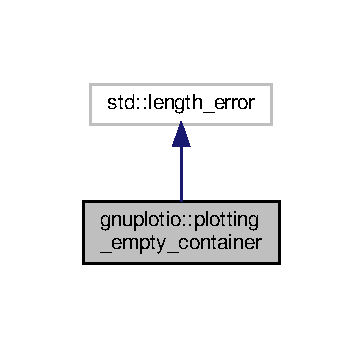
\includegraphics[width=174pt]{classgnuplotio_1_1plotting__empty__container__inherit__graph}
\end{center}
\end{figure}


Collaboration diagram for gnuplotio\+:\+:plotting\+\_\+empty\+\_\+container\+:\nopagebreak
\begin{figure}[H]
\begin{center}
\leavevmode
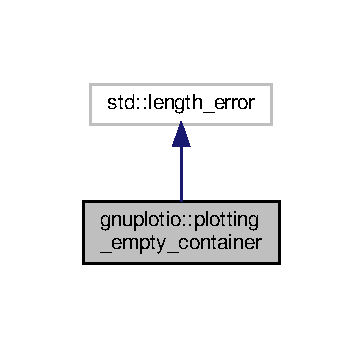
\includegraphics[width=174pt]{classgnuplotio_1_1plotting__empty__container__coll__graph}
\end{center}
\end{figure}


The documentation for this class was generated from the following file\+:\begin{DoxyCompactItemize}
\item 
include/gnuplot-\/iostream.\+h\end{DoxyCompactItemize}

\hypertarget{structgnuplotio_1_1TextSender}{}\section{gnuplotio\+:\+:Text\+Sender$<$ T, Enable $>$ Struct Template Reference}
\label{structgnuplotio_1_1TextSender}\index{gnuplotio\+::\+Text\+Sender$<$ T, Enable $>$@{gnuplotio\+::\+Text\+Sender$<$ T, Enable $>$}}
\subsection*{Static Public Member Functions}
\begin{DoxyCompactItemize}
\item 
\mbox{\Hypertarget{structgnuplotio_1_1TextSender_a03b58292dc75a4137d30ad7fffd762c6}\label{structgnuplotio_1_1TextSender_a03b58292dc75a4137d30ad7fffd762c6}} 
static void {\bfseries send} (std\+::ostream \&stream, const T \&v)
\end{DoxyCompactItemize}


The documentation for this struct was generated from the following file\+:\begin{DoxyCompactItemize}
\item 
include/gnuplot-\/iostream.\+h\end{DoxyCompactItemize}

\hypertarget{structgnuplotio_1_1TextSender_3_01char_01_4}{}\section{gnuplotio\+:\+:Text\+Sender$<$ char $>$ Struct Template Reference}
\label{structgnuplotio_1_1TextSender_3_01char_01_4}\index{gnuplotio\+::\+Text\+Sender$<$ char $>$@{gnuplotio\+::\+Text\+Sender$<$ char $>$}}


Inheritance diagram for gnuplotio\+:\+:Text\+Sender$<$ char $>$\+:\nopagebreak
\begin{figure}[H]
\begin{center}
\leavevmode
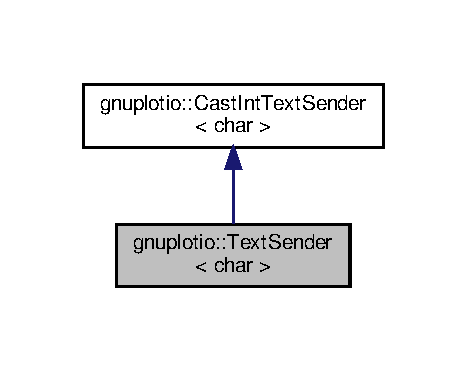
\includegraphics[width=224pt]{structgnuplotio_1_1TextSender_3_01char_01_4__inherit__graph}
\end{center}
\end{figure}


Collaboration diagram for gnuplotio\+:\+:Text\+Sender$<$ char $>$\+:\nopagebreak
\begin{figure}[H]
\begin{center}
\leavevmode
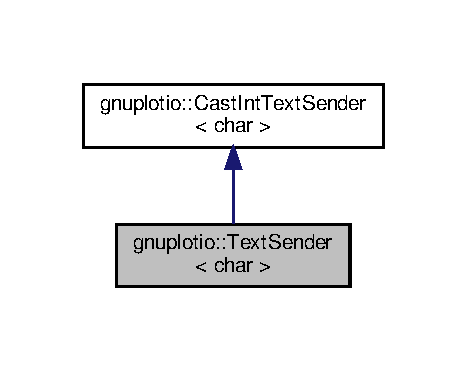
\includegraphics[width=224pt]{structgnuplotio_1_1TextSender_3_01char_01_4__coll__graph}
\end{center}
\end{figure}
\subsection*{Additional Inherited Members}


The documentation for this struct was generated from the following file\+:\begin{DoxyCompactItemize}
\item 
include/gnuplot-\/iostream.\+h\end{DoxyCompactItemize}

\hypertarget{structgnuplotio_1_1TextSender_3_01double_01_4}{}\section{gnuplotio\+:\+:Text\+Sender$<$ double $>$ Struct Template Reference}
\label{structgnuplotio_1_1TextSender_3_01double_01_4}\index{gnuplotio\+::\+Text\+Sender$<$ double $>$@{gnuplotio\+::\+Text\+Sender$<$ double $>$}}


Inheritance diagram for gnuplotio\+:\+:Text\+Sender$<$ double $>$\+:\nopagebreak
\begin{figure}[H]
\begin{center}
\leavevmode
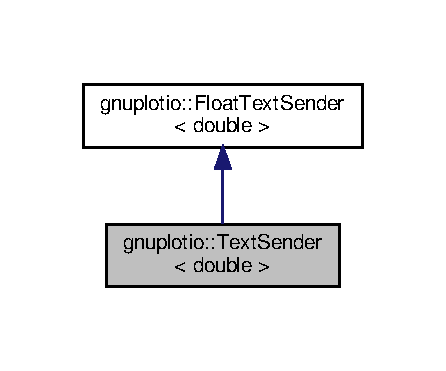
\includegraphics[width=214pt]{structgnuplotio_1_1TextSender_3_01double_01_4__inherit__graph}
\end{center}
\end{figure}


Collaboration diagram for gnuplotio\+:\+:Text\+Sender$<$ double $>$\+:\nopagebreak
\begin{figure}[H]
\begin{center}
\leavevmode
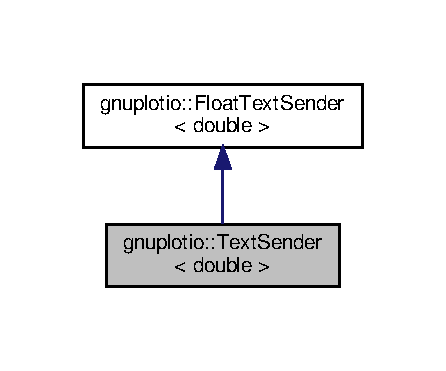
\includegraphics[width=214pt]{structgnuplotio_1_1TextSender_3_01double_01_4__coll__graph}
\end{center}
\end{figure}
\subsection*{Additional Inherited Members}


The documentation for this struct was generated from the following file\+:\begin{DoxyCompactItemize}
\item 
include/gnuplot-\/iostream.\+h\end{DoxyCompactItemize}

\hypertarget{structgnuplotio_1_1TextSender_3_01float_01_4}{}\section{gnuplotio\+:\+:Text\+Sender$<$ float $>$ Struct Template Reference}
\label{structgnuplotio_1_1TextSender_3_01float_01_4}\index{gnuplotio\+::\+Text\+Sender$<$ float $>$@{gnuplotio\+::\+Text\+Sender$<$ float $>$}}


Inheritance diagram for gnuplotio\+:\+:Text\+Sender$<$ float $>$\+:\nopagebreak
\begin{figure}[H]
\begin{center}
\leavevmode
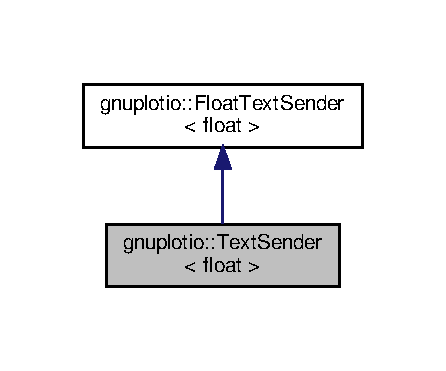
\includegraphics[width=214pt]{structgnuplotio_1_1TextSender_3_01float_01_4__inherit__graph}
\end{center}
\end{figure}


Collaboration diagram for gnuplotio\+:\+:Text\+Sender$<$ float $>$\+:\nopagebreak
\begin{figure}[H]
\begin{center}
\leavevmode
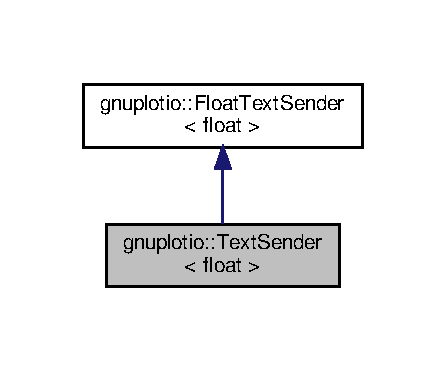
\includegraphics[width=214pt]{structgnuplotio_1_1TextSender_3_01float_01_4__coll__graph}
\end{center}
\end{figure}
\subsection*{Additional Inherited Members}


The documentation for this struct was generated from the following file\+:\begin{DoxyCompactItemize}
\item 
include/gnuplot-\/iostream.\+h\end{DoxyCompactItemize}

\hypertarget{structgnuplotio_1_1TextSender_3_01long_01double_01_4}{}\section{gnuplotio\+:\+:Text\+Sender$<$ long double $>$ Struct Template Reference}
\label{structgnuplotio_1_1TextSender_3_01long_01double_01_4}\index{gnuplotio\+::\+Text\+Sender$<$ long double $>$@{gnuplotio\+::\+Text\+Sender$<$ long double $>$}}


Inheritance diagram for gnuplotio\+:\+:Text\+Sender$<$ long double $>$\+:\nopagebreak
\begin{figure}[H]
\begin{center}
\leavevmode
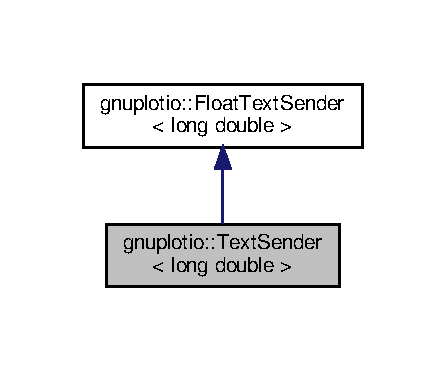
\includegraphics[width=214pt]{structgnuplotio_1_1TextSender_3_01long_01double_01_4__inherit__graph}
\end{center}
\end{figure}


Collaboration diagram for gnuplotio\+:\+:Text\+Sender$<$ long double $>$\+:\nopagebreak
\begin{figure}[H]
\begin{center}
\leavevmode
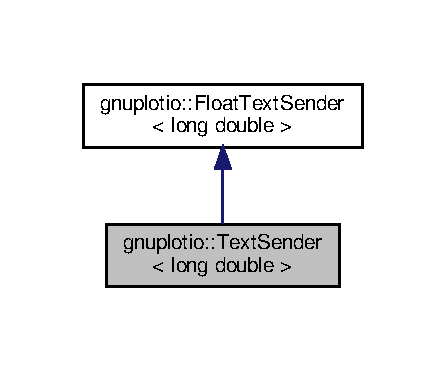
\includegraphics[width=214pt]{structgnuplotio_1_1TextSender_3_01long_01double_01_4__coll__graph}
\end{center}
\end{figure}
\subsection*{Additional Inherited Members}


The documentation for this struct was generated from the following file\+:\begin{DoxyCompactItemize}
\item 
include/gnuplot-\/iostream.\+h\end{DoxyCompactItemize}

\hypertarget{structgnuplotio_1_1TextSender_3_01signed_01char_01_4}{}\section{gnuplotio\+:\+:Text\+Sender$<$ signed char $>$ Struct Template Reference}
\label{structgnuplotio_1_1TextSender_3_01signed_01char_01_4}\index{gnuplotio\+::\+Text\+Sender$<$ signed char $>$@{gnuplotio\+::\+Text\+Sender$<$ signed char $>$}}


Inheritance diagram for gnuplotio\+:\+:Text\+Sender$<$ signed char $>$\+:\nopagebreak
\begin{figure}[H]
\begin{center}
\leavevmode
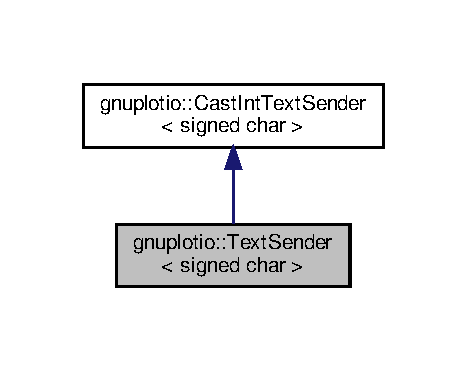
\includegraphics[width=224pt]{structgnuplotio_1_1TextSender_3_01signed_01char_01_4__inherit__graph}
\end{center}
\end{figure}


Collaboration diagram for gnuplotio\+:\+:Text\+Sender$<$ signed char $>$\+:\nopagebreak
\begin{figure}[H]
\begin{center}
\leavevmode
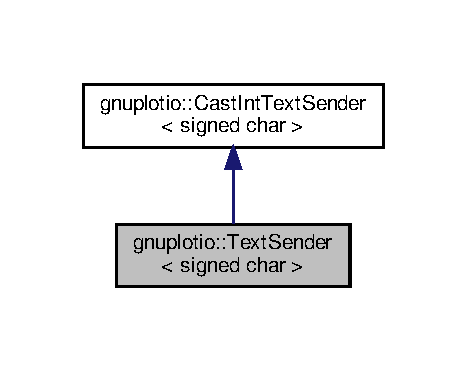
\includegraphics[width=224pt]{structgnuplotio_1_1TextSender_3_01signed_01char_01_4__coll__graph}
\end{center}
\end{figure}
\subsection*{Additional Inherited Members}


The documentation for this struct was generated from the following file\+:\begin{DoxyCompactItemize}
\item 
include/gnuplot-\/iostream.\+h\end{DoxyCompactItemize}

\hypertarget{structgnuplotio_1_1TextSender_3_01std_1_1complex_3_01T_01_4_01_4}{}\section{gnuplotio\+:\+:Text\+Sender$<$ std\+:\+:complex$<$ T $>$ $>$ Struct Template Reference}
\label{structgnuplotio_1_1TextSender_3_01std_1_1complex_3_01T_01_4_01_4}\index{gnuplotio\+::\+Text\+Sender$<$ std\+::complex$<$ T $>$ $>$@{gnuplotio\+::\+Text\+Sender$<$ std\+::complex$<$ T $>$ $>$}}
\subsection*{Static Public Member Functions}
\begin{DoxyCompactItemize}
\item 
\mbox{\Hypertarget{structgnuplotio_1_1TextSender_3_01std_1_1complex_3_01T_01_4_01_4_ad524aa3e121d0ebd66346d77f1fd5a1c}\label{structgnuplotio_1_1TextSender_3_01std_1_1complex_3_01T_01_4_01_4_ad524aa3e121d0ebd66346d77f1fd5a1c}} 
static void {\bfseries send} (std\+::ostream \&stream, const std\+::complex$<$ T $>$ \&v)
\end{DoxyCompactItemize}


The documentation for this struct was generated from the following file\+:\begin{DoxyCompactItemize}
\item 
include/gnuplot-\/iostream.\+h\end{DoxyCompactItemize}

\hypertarget{structgnuplotio_1_1TextSender_3_01std_1_1pair_3_01T_00_01U_01_4_01_4}{}\section{gnuplotio\+:\+:Text\+Sender$<$ std\+:\+:pair$<$ T, U $>$ $>$ Struct Template Reference}
\label{structgnuplotio_1_1TextSender_3_01std_1_1pair_3_01T_00_01U_01_4_01_4}\index{gnuplotio\+::\+Text\+Sender$<$ std\+::pair$<$ T, U $>$ $>$@{gnuplotio\+::\+Text\+Sender$<$ std\+::pair$<$ T, U $>$ $>$}}
\subsection*{Static Public Member Functions}
\begin{DoxyCompactItemize}
\item 
\mbox{\Hypertarget{structgnuplotio_1_1TextSender_3_01std_1_1pair_3_01T_00_01U_01_4_01_4_ae1f3a6ffd8a60bb73d787578327154d1}\label{structgnuplotio_1_1TextSender_3_01std_1_1pair_3_01T_00_01U_01_4_01_4_ae1f3a6ffd8a60bb73d787578327154d1}} 
static void {\bfseries send} (std\+::ostream \&stream, const std\+::pair$<$ T, U $>$ \&v)
\end{DoxyCompactItemize}


The documentation for this struct was generated from the following file\+:\begin{DoxyCompactItemize}
\item 
include/gnuplot-\/iostream.\+h\end{DoxyCompactItemize}

\hypertarget{structgnuplotio_1_1TextSender_3_01T_00_01typename_01boost_1_1enable__if_3_01boost_1_1mpl_1_1and_613e8c35e9263a9c4b5e2b75ff99b434}{}\section{gnuplotio\+:\+:Text\+Sender$<$ T, typename boost\+:\+:enable\+\_\+if$<$ boost\+:\+:mpl\+:\+:and\+\_\+$<$ is\+\_\+boost\+\_\+tuple$<$ T $>$, boost\+:\+:mpl\+:\+:not\+\_\+$<$ is\+\_\+boost\+\_\+tuple\+\_\+nulltype$<$ typename T\+:\+:tail\+\_\+type $>$ $>$ $>$ $>$\+:\+:type $>$ Struct Template Reference}
\label{structgnuplotio_1_1TextSender_3_01T_00_01typename_01boost_1_1enable__if_3_01boost_1_1mpl_1_1and_613e8c35e9263a9c4b5e2b75ff99b434}\index{gnuplotio\+::\+Text\+Sender$<$ T, typename boost\+::enable\+\_\+if$<$ boost\+::mpl\+::and\+\_\+$<$ is\+\_\+boost\+\_\+tuple$<$ T $>$, boost\+::mpl\+::not\+\_\+$<$ is\+\_\+boost\+\_\+tuple\+\_\+nulltype$<$ typename T\+::tail\+\_\+type $>$ $>$ $>$ $>$\+::type $>$@{gnuplotio\+::\+Text\+Sender$<$ T, typename boost\+::enable\+\_\+if$<$ boost\+::mpl\+::and\+\_\+$<$ is\+\_\+boost\+\_\+tuple$<$ T $>$, boost\+::mpl\+::not\+\_\+$<$ is\+\_\+boost\+\_\+tuple\+\_\+nulltype$<$ typename T\+::tail\+\_\+type $>$ $>$ $>$ $>$\+::type $>$}}
\subsection*{Static Public Member Functions}
\begin{DoxyCompactItemize}
\item 
\mbox{\Hypertarget{structgnuplotio_1_1TextSender_3_01T_00_01typename_01boost_1_1enable__if_3_01boost_1_1mpl_1_1and_613e8c35e9263a9c4b5e2b75ff99b434_a57bf894398f70f08cd4bac18ee5cbf68}\label{structgnuplotio_1_1TextSender_3_01T_00_01typename_01boost_1_1enable__if_3_01boost_1_1mpl_1_1and_613e8c35e9263a9c4b5e2b75ff99b434_a57bf894398f70f08cd4bac18ee5cbf68}} 
static void {\bfseries send} (std\+::ostream \&stream, const T \&v)
\end{DoxyCompactItemize}


The documentation for this struct was generated from the following file\+:\begin{DoxyCompactItemize}
\item 
include/gnuplot-\/iostream.\+h\end{DoxyCompactItemize}

\hypertarget{structgnuplotio_1_1TextSender_3_01T_00_01typename_01boost_1_1enable__if_3_01boost_1_1mpl_1_1and_bf5c774ba95be74c5a1a563b931819fa}{}\section{gnuplotio\+:\+:Text\+Sender$<$ T, typename boost\+:\+:enable\+\_\+if$<$ boost\+:\+:mpl\+:\+:and\+\_\+$<$ is\+\_\+boost\+\_\+tuple$<$ T $>$, is\+\_\+boost\+\_\+tuple\+\_\+nulltype$<$ typename T\+:\+:tail\+\_\+type $>$ $>$ $>$\+:\+:type $>$ Struct Template Reference}
\label{structgnuplotio_1_1TextSender_3_01T_00_01typename_01boost_1_1enable__if_3_01boost_1_1mpl_1_1and_bf5c774ba95be74c5a1a563b931819fa}\index{gnuplotio\+::\+Text\+Sender$<$ T, typename boost\+::enable\+\_\+if$<$ boost\+::mpl\+::and\+\_\+$<$ is\+\_\+boost\+\_\+tuple$<$ T $>$, is\+\_\+boost\+\_\+tuple\+\_\+nulltype$<$ typename T\+::tail\+\_\+type $>$ $>$ $>$\+::type $>$@{gnuplotio\+::\+Text\+Sender$<$ T, typename boost\+::enable\+\_\+if$<$ boost\+::mpl\+::and\+\_\+$<$ is\+\_\+boost\+\_\+tuple$<$ T $>$, is\+\_\+boost\+\_\+tuple\+\_\+nulltype$<$ typename T\+::tail\+\_\+type $>$ $>$ $>$\+::type $>$}}
\subsection*{Static Public Member Functions}
\begin{DoxyCompactItemize}
\item 
\mbox{\Hypertarget{structgnuplotio_1_1TextSender_3_01T_00_01typename_01boost_1_1enable__if_3_01boost_1_1mpl_1_1and_bf5c774ba95be74c5a1a563b931819fa_a76a476180ea04c950c1cfdb71c556525}\label{structgnuplotio_1_1TextSender_3_01T_00_01typename_01boost_1_1enable__if_3_01boost_1_1mpl_1_1and_bf5c774ba95be74c5a1a563b931819fa_a76a476180ea04c950c1cfdb71c556525}} 
static void {\bfseries send} (std\+::ostream \&stream, const T \&v)
\end{DoxyCompactItemize}


The documentation for this struct was generated from the following file\+:\begin{DoxyCompactItemize}
\item 
include/gnuplot-\/iostream.\+h\end{DoxyCompactItemize}

\hypertarget{structgnuplotio_1_1TextSender_3_01unsigned_01char_01_4}{}\section{gnuplotio\+:\+:Text\+Sender$<$ unsigned char $>$ Struct Template Reference}
\label{structgnuplotio_1_1TextSender_3_01unsigned_01char_01_4}\index{gnuplotio\+::\+Text\+Sender$<$ unsigned char $>$@{gnuplotio\+::\+Text\+Sender$<$ unsigned char $>$}}


Inheritance diagram for gnuplotio\+:\+:Text\+Sender$<$ unsigned char $>$\+:\nopagebreak
\begin{figure}[H]
\begin{center}
\leavevmode
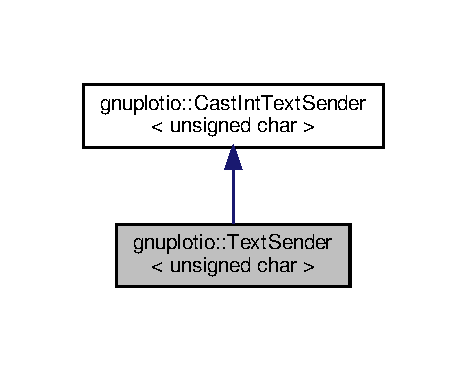
\includegraphics[width=224pt]{structgnuplotio_1_1TextSender_3_01unsigned_01char_01_4__inherit__graph}
\end{center}
\end{figure}


Collaboration diagram for gnuplotio\+:\+:Text\+Sender$<$ unsigned char $>$\+:\nopagebreak
\begin{figure}[H]
\begin{center}
\leavevmode
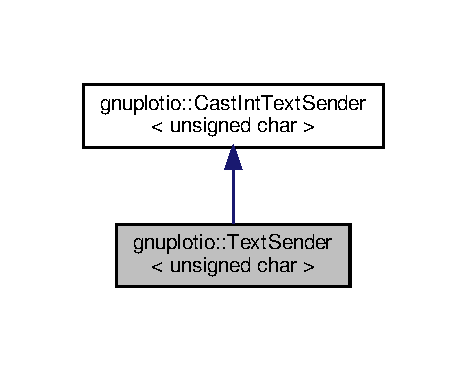
\includegraphics[width=224pt]{structgnuplotio_1_1TextSender_3_01unsigned_01char_01_4__coll__graph}
\end{center}
\end{figure}
\subsection*{Additional Inherited Members}


The documentation for this struct was generated from the following file\+:\begin{DoxyCompactItemize}
\item 
include/gnuplot-\/iostream.\+h\end{DoxyCompactItemize}

\hypertarget{classTwoWDRobot}{}\section{Two\+W\+D\+Robot Class Reference}
\label{classTwoWDRobot}\index{Two\+W\+D\+Robot@{Two\+W\+D\+Robot}}


Implementation of an \hyperlink{classTwoWDRobot}{Two\+W\+D\+Robot} Class.  




{\ttfamily \#include $<$two\+W\+D\+Robot.\+hpp$>$}

\subsection*{Public Member Functions}
\begin{DoxyCompactItemize}
\item 
\mbox{\Hypertarget{classTwoWDRobot_a55b4deb35b13238caf8e3e9d9683f7fc}\label{classTwoWDRobot_a55b4deb35b13238caf8e3e9d9683f7fc}} 
\hyperlink{classTwoWDRobot_a55b4deb35b13238caf8e3e9d9683f7fc}{Two\+W\+D\+Robot} ()
\begin{DoxyCompactList}\small\item\em Constructor for \hyperlink{classTwoWDRobot}{Two\+W\+D\+Robot} class. \end{DoxyCompactList}\item 
\mbox{\Hypertarget{classTwoWDRobot_a8fb430bcff3260b0cc87b2ac394cafec}\label{classTwoWDRobot_a8fb430bcff3260b0cc87b2ac394cafec}} 
\hyperlink{classTwoWDRobot_a8fb430bcff3260b0cc87b2ac394cafec}{$\sim$\+Two\+W\+D\+Robot} ()
\begin{DoxyCompactList}\small\item\em Destructor for \hyperlink{classTwoWDRobot}{Two\+W\+D\+Robot} class. \end{DoxyCompactList}\item 
bool \hyperlink{classTwoWDRobot_a2ad1824258f39b02e9cd034589b96c4d}{set\+Target\+Heading} (double \+\_\+target\+Heading)
\begin{DoxyCompactList}\small\item\em Setter for Target Heading. \end{DoxyCompactList}\item 
bool \hyperlink{classTwoWDRobot_a5793dfd8c9b217ee1a811b1bb0460c25}{set\+Target\+Velocity} (double \+\_\+target\+Velocity)
\begin{DoxyCompactList}\small\item\em Setter for target Velocity. \end{DoxyCompactList}\item 
bool \hyperlink{classTwoWDRobot_a5b462497a3776817763f0ec48a887e26}{compute\+Output} (double initial\+Heading, double initial\+Velocity, bool flag)
\begin{DoxyCompactList}\small\item\em method to compute the outputs \end{DoxyCompactList}\end{DoxyCompactItemize}


\subsection{Detailed Description}
Implementation of an \hyperlink{classTwoWDRobot}{Two\+W\+D\+Robot} Class. 

\subsection{Member Function Documentation}
\mbox{\Hypertarget{classTwoWDRobot_a5b462497a3776817763f0ec48a887e26}\label{classTwoWDRobot_a5b462497a3776817763f0ec48a887e26}} 
\index{Two\+W\+D\+Robot@{Two\+W\+D\+Robot}!compute\+Output@{compute\+Output}}
\index{compute\+Output@{compute\+Output}!Two\+W\+D\+Robot@{Two\+W\+D\+Robot}}
\subsubsection{\texorpdfstring{compute\+Output()}{computeOutput()}}
{\footnotesize\ttfamily bool Two\+W\+D\+Robot\+::compute\+Output (\begin{DoxyParamCaption}\item[{double}]{initial\+Heading,  }\item[{double}]{initial\+Velocity,  }\item[{bool}]{flag }\end{DoxyParamCaption})}



method to compute the outputs 


\begin{DoxyParams}[1]{Parameters}
\mbox{\tt in}  & {\em initial\+Heading} & Initial Heading \\
\hline
\mbox{\tt in}  & {\em initial\+Velocity} & Initial Velocity of the robot \\
\hline
\mbox{\tt in}  & {\em flag} & flag for testing \\
\hline
\end{DoxyParams}
\begin{DoxyReturn}{Returns}
true/false 
\end{DoxyReturn}
\mbox{\Hypertarget{classTwoWDRobot_a2ad1824258f39b02e9cd034589b96c4d}\label{classTwoWDRobot_a2ad1824258f39b02e9cd034589b96c4d}} 
\index{Two\+W\+D\+Robot@{Two\+W\+D\+Robot}!set\+Target\+Heading@{set\+Target\+Heading}}
\index{set\+Target\+Heading@{set\+Target\+Heading}!Two\+W\+D\+Robot@{Two\+W\+D\+Robot}}
\subsubsection{\texorpdfstring{set\+Target\+Heading()}{setTargetHeading()}}
{\footnotesize\ttfamily bool Two\+W\+D\+Robot\+::set\+Target\+Heading (\begin{DoxyParamCaption}\item[{double}]{\+\_\+target\+Heading }\end{DoxyParamCaption})}



Setter for Target Heading. 


\begin{DoxyParams}[1]{Parameters}
\mbox{\tt in}  & {\em \+\_\+targetheading} & target heading of the robot \\
\hline
\end{DoxyParams}
\begin{DoxyReturn}{Returns}
true/false 
\end{DoxyReturn}
\mbox{\Hypertarget{classTwoWDRobot_a5793dfd8c9b217ee1a811b1bb0460c25}\label{classTwoWDRobot_a5793dfd8c9b217ee1a811b1bb0460c25}} 
\index{Two\+W\+D\+Robot@{Two\+W\+D\+Robot}!set\+Target\+Velocity@{set\+Target\+Velocity}}
\index{set\+Target\+Velocity@{set\+Target\+Velocity}!Two\+W\+D\+Robot@{Two\+W\+D\+Robot}}
\subsubsection{\texorpdfstring{set\+Target\+Velocity()}{setTargetVelocity()}}
{\footnotesize\ttfamily bool Two\+W\+D\+Robot\+::set\+Target\+Velocity (\begin{DoxyParamCaption}\item[{double}]{\+\_\+target\+Velocity }\end{DoxyParamCaption})}



Setter for target Velocity. 


\begin{DoxyParams}[1]{Parameters}
\mbox{\tt in}  & {\em \+\_\+target\+Velocity} & target Velocity of the robot \\
\hline
\end{DoxyParams}
\begin{DoxyReturn}{Returns}
true/false 
\end{DoxyReturn}


The documentation for this class was generated from the following files\+:\begin{DoxyCompactItemize}
\item 
include/\hyperlink{twoWDRobot_8hpp}{two\+W\+D\+Robot.\+hpp}\item 
app/\hyperlink{twoWDRobot_8cpp}{two\+W\+D\+Robot.\+cpp}\end{DoxyCompactItemize}

\hypertarget{structgnuplotio_1_1ModeAutoDecoder_1_1type_01_4}{}\section{gnuplotio\+:\+:Mode\+Auto\+Decoder$<$ T, Enable $>$\+:\+:type $>$ Struct Reference}
\label{structgnuplotio_1_1ModeAutoDecoder_1_1type_01_4}\index{gnuplotio\+::\+Mode\+Auto\+Decoder$<$ T, Enable $>$\+::type $>$@{gnuplotio\+::\+Mode\+Auto\+Decoder$<$ T, Enable $>$\+::type $>$}}
\subsection*{Public Types}
\begin{DoxyCompactItemize}
\item 
\mbox{\Hypertarget{structgnuplotio_1_1ModeAutoDecoder_1_1type_01_4_ad1942745c810b24503495c6ade6bd9f6}\label{structgnuplotio_1_1ModeAutoDecoder_1_1type_01_4_ad1942745c810b24503495c6ade6bd9f6}} 
typedef \hyperlink{structgnuplotio_1_1Mode2DUnwrap}{Mode2\+D\+Unwrap} {\bfseries mode}
\item 
\mbox{\Hypertarget{structgnuplotio_1_1ModeAutoDecoder_1_1type_01_4_a07e8af1d93e8107efb7be6fd68b0024c}\label{structgnuplotio_1_1ModeAutoDecoder_1_1type_01_4_a07e8af1d93e8107efb7be6fd68b0024c}} 
typedef \hyperlink{structgnuplotio_1_1Mode2D}{Mode2D} {\bfseries mode}
\end{DoxyCompactItemize}


The documentation for this struct was generated from the following file\+:\begin{DoxyCompactItemize}
\item 
include/gnuplot-\/iostream.\+h\end{DoxyCompactItemize}

\hypertarget{classgnuplotio_1_1VecOfRange}{}\section{gnuplotio\+:\+:Vec\+Of\+Range$<$ RT $>$ Class Template Reference}
\label{classgnuplotio_1_1VecOfRange}\index{gnuplotio\+::\+Vec\+Of\+Range$<$ R\+T $>$@{gnuplotio\+::\+Vec\+Of\+Range$<$ R\+T $>$}}
\subsection*{Public Types}
\begin{DoxyCompactItemize}
\item 
\mbox{\Hypertarget{classgnuplotio_1_1VecOfRange_aed503f2f8d8ed71b303f2db26872bafd}\label{classgnuplotio_1_1VecOfRange_aed503f2f8d8ed71b303f2db26872bafd}} 
typedef std\+::vector$<$ typename R\+T\+::value\+\_\+type $>$ {\bfseries value\+\_\+type}
\item 
\mbox{\Hypertarget{classgnuplotio_1_1VecOfRange_a4cfae20b9797febceffafec3415b52db}\label{classgnuplotio_1_1VecOfRange_a4cfae20b9797febceffafec3415b52db}} 
typedef \hyperlink{classgnuplotio_1_1VecOfRange}{Vec\+Of\+Range}$<$ typename R\+T\+::subiter\+\_\+type $>$ {\bfseries subiter\+\_\+type}
\end{DoxyCompactItemize}
\subsection*{Public Member Functions}
\begin{DoxyCompactItemize}
\item 
\mbox{\Hypertarget{classgnuplotio_1_1VecOfRange_a81e04f9ab4b8641d69df61f695e97e34}\label{classgnuplotio_1_1VecOfRange_a81e04f9ab4b8641d69df61f695e97e34}} 
{\bfseries Vec\+Of\+Range} (const std\+::vector$<$ RT $>$ \&\+\_\+rvec)
\item 
\mbox{\Hypertarget{classgnuplotio_1_1VecOfRange_a714b945004e06909e5a0cdc3cca619b5}\label{classgnuplotio_1_1VecOfRange_a714b945004e06909e5a0cdc3cca619b5}} 
bool {\bfseries is\+\_\+end} () const
\item 
\mbox{\Hypertarget{classgnuplotio_1_1VecOfRange_a2e5371ab6c88994e3fc6f12324783e1c}\label{classgnuplotio_1_1VecOfRange_a2e5371ab6c88994e3fc6f12324783e1c}} 
void {\bfseries inc} ()
\item 
\mbox{\Hypertarget{classgnuplotio_1_1VecOfRange_ab0a35bc07a4f12b18bd1541bc4b771fc}\label{classgnuplotio_1_1VecOfRange_ab0a35bc07a4f12b18bd1541bc4b771fc}} 
value\+\_\+type {\bfseries deref} () const
\item 
\mbox{\Hypertarget{classgnuplotio_1_1VecOfRange_a9b02d8bd8ec62ba77de16ad8ea8a87b2}\label{classgnuplotio_1_1VecOfRange_a9b02d8bd8ec62ba77de16ad8ea8a87b2}} 
\hyperlink{classgnuplotio_1_1VecOfRange}{subiter\+\_\+type} {\bfseries deref\+\_\+subiter} () const
\end{DoxyCompactItemize}
\subsection*{Static Public Attributes}
\begin{DoxyCompactItemize}
\item 
\mbox{\Hypertarget{classgnuplotio_1_1VecOfRange_a8725d4907d46575dddb7152f1f1d1f66}\label{classgnuplotio_1_1VecOfRange_a8725d4907d46575dddb7152f1f1d1f66}} 
static const bool {\bfseries is\+\_\+container} = R\+T\+::is\+\_\+container
\item 
\mbox{\Hypertarget{classgnuplotio_1_1VecOfRange_a19d87e61a7854f9e22d3dd8a94f79500}\label{classgnuplotio_1_1VecOfRange_a19d87e61a7854f9e22d3dd8a94f79500}} 
static const bool {\bfseries allow\+\_\+auto\+\_\+unwrap} = false
\end{DoxyCompactItemize}
\subsection*{Friends}
\begin{DoxyCompactItemize}
\item 
\mbox{\Hypertarget{classgnuplotio_1_1VecOfRange_adafbfb0122b8e499d1af9c246f4ac288}\label{classgnuplotio_1_1VecOfRange_adafbfb0122b8e499d1af9c246f4ac288}} 
{\footnotesize template$<$typename T , typename Print\+Mode $>$ }\\void {\bfseries deref\+\_\+and\+\_\+print} (std\+::ostream \&, const \hyperlink{classgnuplotio_1_1VecOfRange}{Vec\+Of\+Range}$<$ T $>$ \&, Print\+Mode)
\end{DoxyCompactItemize}


The documentation for this class was generated from the following file\+:\begin{DoxyCompactItemize}
\item 
include/gnuplot-\/iostream.\+h\end{DoxyCompactItemize}

\hypertarget{classVisualization}{}\section{Visualization Class Reference}
\label{classVisualization}\index{Visualization@{Visualization}}


Implementation of an \hyperlink{classVisualization}{Visualization} Class.  




{\ttfamily \#include $<$visualization.\+hpp$>$}

\subsection*{Public Member Functions}
\begin{DoxyCompactItemize}
\item 
bool \hyperlink{classVisualization_a5a77f1a16a69153aa4671e8c56e1cbc9}{set\+Velocities} (std\+::vector$<$ double $>$ v)
\item 
bool \hyperlink{classVisualization_a012238010c15a864fe592de3c8a6a7fa}{set\+Headings} (std\+::vector$<$ double $>$ h)
\item 
bool \hyperlink{classVisualization_a39cc1a94ab49ffc11a1542ef9646858a}{set\+Time} (std\+::vector$<$ double $>$ t)
\item 
bool \hyperlink{classVisualization_a91068dbd17952cf42439b377f1a2b1ca}{plot\+Velocities} (std\+::vector$<$ double $>$ \+\_\+velocities, std\+::vector$<$ double $>$ \+\_\+time)
\begin{DoxyCompactList}\small\item\em plots velocity vs time graph \end{DoxyCompactList}\item 
bool \hyperlink{classVisualization_a6896d287f4575a5ccc5a4370e36dbb19}{plot\+Headings} (std\+::vector$<$ double $>$ \+\_\+headings, std\+::vector$<$ double $>$ \+\_\+time)
\begin{DoxyCompactList}\small\item\em plots heading vs time graph \end{DoxyCompactList}\end{DoxyCompactItemize}


\subsection{Detailed Description}
Implementation of an \hyperlink{classVisualization}{Visualization} Class. 

\subsection{Member Function Documentation}
\mbox{\Hypertarget{classVisualization_a6896d287f4575a5ccc5a4370e36dbb19}\label{classVisualization_a6896d287f4575a5ccc5a4370e36dbb19}} 
\index{Visualization@{Visualization}!plot\+Headings@{plot\+Headings}}
\index{plot\+Headings@{plot\+Headings}!Visualization@{Visualization}}
\subsubsection{\texorpdfstring{plot\+Headings()}{plotHeadings()}}
{\footnotesize\ttfamily bool Visualization\+::plot\+Headings (\begin{DoxyParamCaption}\item[{std\+::vector$<$ double $>$}]{\+\_\+headings,  }\item[{std\+::vector$<$ double $>$}]{\+\_\+time }\end{DoxyParamCaption})}



plots heading vs time graph 


\begin{DoxyParams}[1]{Parameters}
\mbox{\tt in}  & {\em \+\_\+headings} & vector of headings \\
\hline
\mbox{\tt in}  & {\em \+\_\+time} & vector of time \\
\hline
\end{DoxyParams}
\begin{DoxyReturn}{Returns}
true/false 
\end{DoxyReturn}
\mbox{\Hypertarget{classVisualization_a91068dbd17952cf42439b377f1a2b1ca}\label{classVisualization_a91068dbd17952cf42439b377f1a2b1ca}} 
\index{Visualization@{Visualization}!plot\+Velocities@{plot\+Velocities}}
\index{plot\+Velocities@{plot\+Velocities}!Visualization@{Visualization}}
\subsubsection{\texorpdfstring{plot\+Velocities()}{plotVelocities()}}
{\footnotesize\ttfamily bool Visualization\+::plot\+Velocities (\begin{DoxyParamCaption}\item[{std\+::vector$<$ double $>$}]{\+\_\+velocities,  }\item[{std\+::vector$<$ double $>$}]{\+\_\+time }\end{DoxyParamCaption})}



plots velocity vs time graph 


\begin{DoxyParams}[1]{Parameters}
\mbox{\tt in}  & {\em \+\_\+velocities} & vector of velocities \\
\hline
\mbox{\tt in}  & {\em \+\_\+time} & vector of time \\
\hline
\end{DoxyParams}
\begin{DoxyReturn}{Returns}
true/false 
\end{DoxyReturn}
\mbox{\Hypertarget{classVisualization_a012238010c15a864fe592de3c8a6a7fa}\label{classVisualization_a012238010c15a864fe592de3c8a6a7fa}} 
\index{Visualization@{Visualization}!set\+Headings@{set\+Headings}}
\index{set\+Headings@{set\+Headings}!Visualization@{Visualization}}
\subsubsection{\texorpdfstring{set\+Headings()}{setHeadings()}}
{\footnotesize\ttfamily bool Visualization\+::set\+Headings (\begin{DoxyParamCaption}\item[{std\+::vector$<$ double $>$}]{h }\end{DoxyParamCaption})}


\begin{DoxyParams}[1]{Parameters}
\mbox{\tt in}  & {\em h} & vector of headings \\
\hline
\end{DoxyParams}
\begin{DoxyReturn}{Returns}
true/false 
\end{DoxyReturn}
\mbox{\Hypertarget{classVisualization_a39cc1a94ab49ffc11a1542ef9646858a}\label{classVisualization_a39cc1a94ab49ffc11a1542ef9646858a}} 
\index{Visualization@{Visualization}!set\+Time@{set\+Time}}
\index{set\+Time@{set\+Time}!Visualization@{Visualization}}
\subsubsection{\texorpdfstring{set\+Time()}{setTime()}}
{\footnotesize\ttfamily bool Visualization\+::set\+Time (\begin{DoxyParamCaption}\item[{std\+::vector$<$ double $>$}]{t }\end{DoxyParamCaption})}


\begin{DoxyParams}[1]{Parameters}
\mbox{\tt in}  & {\em t} & vector of time \\
\hline
\end{DoxyParams}
\begin{DoxyReturn}{Returns}
true/false 
\end{DoxyReturn}
\mbox{\Hypertarget{classVisualization_a5a77f1a16a69153aa4671e8c56e1cbc9}\label{classVisualization_a5a77f1a16a69153aa4671e8c56e1cbc9}} 
\index{Visualization@{Visualization}!set\+Velocities@{set\+Velocities}}
\index{set\+Velocities@{set\+Velocities}!Visualization@{Visualization}}
\subsubsection{\texorpdfstring{set\+Velocities()}{setVelocities()}}
{\footnotesize\ttfamily bool Visualization\+::set\+Velocities (\begin{DoxyParamCaption}\item[{std\+::vector$<$ double $>$}]{v }\end{DoxyParamCaption})}


\begin{DoxyParams}[1]{Parameters}
\mbox{\tt in}  & {\em v} & vector of velocities \\
\hline
\end{DoxyParams}
\begin{DoxyReturn}{Returns}
true/false 
\end{DoxyReturn}


The documentation for this class was generated from the following files\+:\begin{DoxyCompactItemize}
\item 
include/\hyperlink{visualization_8hpp}{visualization.\+hpp}\item 
app/visualization.\+cpp\end{DoxyCompactItemize}

\chapter{File Documentation}
\hypertarget{ackermann_8cpp}{}\section{app/ackermann.cpp File Reference}
\label{ackermann_8cpp}\index{app/ackermann.\+cpp@{app/ackermann.\+cpp}}


Phase1-\/ Driver\+: Vivek Sood Navigator\+: Charu Sharma.  


{\ttfamily \#include \char`\"{}ackermann.\+hpp\char`\"{}}\newline
{\ttfamily \#include $<$math.\+h$>$}\newline
{\ttfamily \#include $<$time.\+h$>$}\newline
{\ttfamily \#include $<$vector$>$}\newline
Include dependency graph for ackermann.\+cpp\+:\nopagebreak
\begin{figure}[H]
\begin{center}
\leavevmode
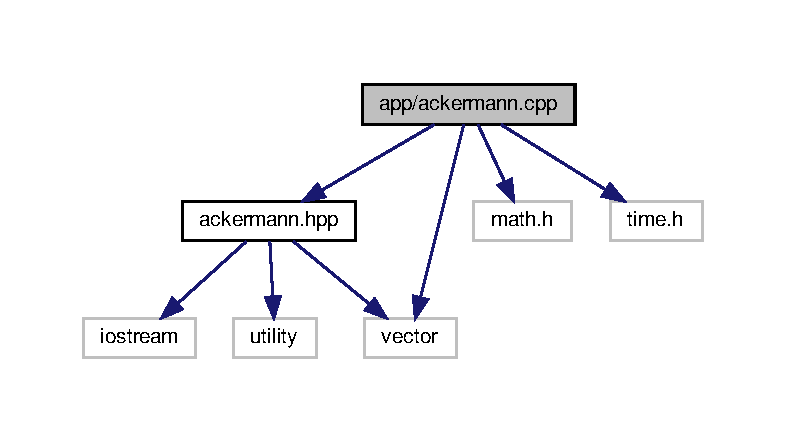
\includegraphics[width=350pt]{ackermann_8cpp__incl}
\end{center}
\end{figure}
\subsection*{Macros}
\begin{DoxyCompactItemize}
\item 
\mbox{\Hypertarget{ackermann_8cpp_a598a3330b3c21701223ee0ca14316eca}\label{ackermann_8cpp_a598a3330b3c21701223ee0ca14316eca}} 
\#define {\bfseries PI}~3.\+141592654
\end{DoxyCompactItemize}


\subsection{Detailed Description}
Phase1-\/ Driver\+: Vivek Sood Navigator\+: Charu Sharma. 

\begin{DoxyAuthor}{Authors}
Vivek Sood, Charu Sharma Phase2-\/ Driver\+: Charu Sharma Navigator\+: Vivek Sood 
\end{DoxyAuthor}

\hypertarget{pid_8cpp}{}\section{app/pid.cpp File Reference}
\label{pid_8cpp}\index{app/pid.\+cpp@{app/pid.\+cpp}}


Driver\+: Vivek Sood Navigator\+: Charu Sharma.  


{\ttfamily \#include $<$pid.\+hpp$>$}\newline
Include dependency graph for pid.\+cpp\+:
\nopagebreak
\begin{figure}[H]
\begin{center}
\leavevmode
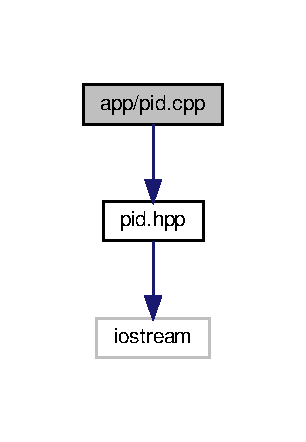
\includegraphics[width=147pt]{pid_8cpp__incl}
\end{center}
\end{figure}


\subsection{Detailed Description}
Driver\+: Vivek Sood Navigator\+: Charu Sharma. 

\begin{DoxyAuthor}{Authors}
Vivek Sood, Charu Sharma 
\end{DoxyAuthor}
\begin{DoxyDate}{Date}
2021-\/10-\/16 
\end{DoxyDate}

\hypertarget{twoWDRobot_8cpp}{}\section{app/two\+W\+D\+Robot.cpp File Reference}
\label{twoWDRobot_8cpp}\index{app/two\+W\+D\+Robot.\+cpp@{app/two\+W\+D\+Robot.\+cpp}}


Driver\+: Vivek Sood Navigator\+: Charu Sharma.  


{\ttfamily \#include \char`\"{}two\+W\+D\+Robot.\+hpp\char`\"{}}\newline
{\ttfamily \#include \char`\"{}pid.\+hpp\char`\"{}}\newline
{\ttfamily \#include \char`\"{}ackermann.\+hpp\char`\"{}}\newline
Include dependency graph for two\+W\+D\+Robot.\+cpp\+:
\nopagebreak
\begin{figure}[H]
\begin{center}
\leavevmode
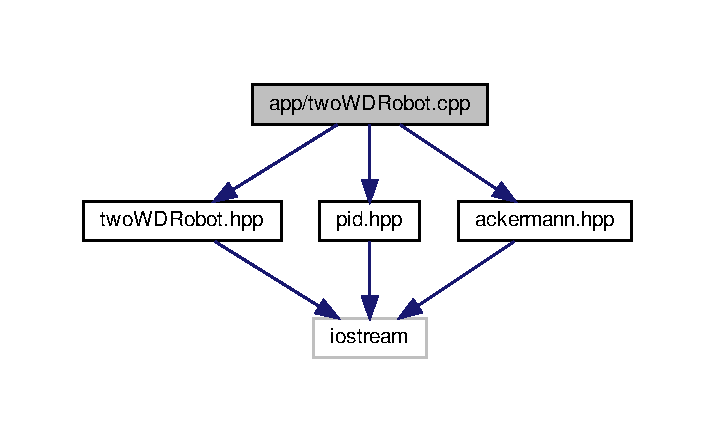
\includegraphics[width=343pt]{twoWDRobot_8cpp__incl}
\end{center}
\end{figure}


\subsection{Detailed Description}
Driver\+: Vivek Sood Navigator\+: Charu Sharma. 

\begin{DoxyAuthor}{Authors}
Vivek Sood, Charu Sharma 
\end{DoxyAuthor}
\begin{DoxyDate}{Date}
2021-\/10-\/16 
\end{DoxyDate}

\hypertarget{visualization_8cpp}{}\section{app/visualization.cpp File Reference}
\label{visualization_8cpp}\index{app/visualization.\+cpp@{app/visualization.\+cpp}}


Phase1-\/ Driver\+: Vivek Sood Navigator\+: Charu Sharma.  


{\ttfamily \#include \char`\"{}visualization.\+hpp\char`\"{}}\newline
{\ttfamily \#include \char`\"{}gnuplot-\/iostream.\+h\char`\"{}}\newline
Include dependency graph for visualization.\+cpp\+:\nopagebreak
\begin{figure}[H]
\begin{center}
\leavevmode
\includegraphics[width=350pt]{visualization_8cpp__incl}
\end{center}
\end{figure}
\subsection*{Macros}
\begin{DoxyCompactItemize}
\item 
\mbox{\Hypertarget{visualization_8cpp_acfbc006ea433ad708fdee3e82996e721}\label{visualization_8cpp_acfbc006ea433ad708fdee3e82996e721}} 
\#define {\bfseries G\+R\+E\+EN}~\char`\"{}\textbackslash{}033\mbox{[}32m\char`\"{}
\item 
\mbox{\Hypertarget{visualization_8cpp_ab702106cf3b3e96750b6845ded4e0299}\label{visualization_8cpp_ab702106cf3b3e96750b6845ded4e0299}} 
\#define {\bfseries R\+E\+S\+ET}~\char`\"{}\textbackslash{}033\mbox{[}0m\char`\"{}
\item 
\mbox{\Hypertarget{visualization_8cpp_abf681265909adf3d3e8116c93c0ba179}\label{visualization_8cpp_abf681265909adf3d3e8116c93c0ba179}} 
\#define {\bfseries Y\+E\+L\+L\+OW}~\char`\"{}\textbackslash{}033\mbox{[}33m\char`\"{}
\end{DoxyCompactItemize}


\subsection{Detailed Description}
Phase1-\/ Driver\+: Vivek Sood Navigator\+: Charu Sharma. 

\begin{DoxyAuthor}{Authors}
Vivek Sood, Charu Sharma Phase2-\/ Driver\+: Charu Sharma Navigator\+: Vivek Sood 
\end{DoxyAuthor}

\hypertarget{ackermann_8hpp}{}\section{include/ackermann.hpp File Reference}
\label{ackermann_8hpp}\index{include/ackermann.\+hpp@{include/ackermann.\+hpp}}


Copyright (c) 2021 Charu Sharma and Vivek Sood.  


{\ttfamily \#include $<$iostream$>$}\newline
{\ttfamily \#include $<$vector$>$}\newline
{\ttfamily \#include $<$utility$>$}\newline
Include dependency graph for ackermann.\+hpp\+:\nopagebreak
\begin{figure}[H]
\begin{center}
\leavevmode
\includegraphics[width=254pt]{ackermann_8hpp__incl}
\end{center}
\end{figure}
This graph shows which files directly or indirectly include this file\+:\nopagebreak
\begin{figure}[H]
\begin{center}
\leavevmode
\includegraphics[width=350pt]{ackermann_8hpp__dep__incl}
\end{center}
\end{figure}
\subsection*{Classes}
\begin{DoxyCompactItemize}
\item 
class \hyperlink{classAckermann}{Ackermann}
\begin{DoxyCompactList}\small\item\em Implementation of an \hyperlink{classAckermann}{Ackermann} Controller. \end{DoxyCompactList}\end{DoxyCompactItemize}


\subsection{Detailed Description}
Copyright (c) 2021 Charu Sharma and Vivek Sood. 

\begin{DoxyAuthor}{Authors}
Vivek Sood, Charu Sharma Phase1-\/ Driver\+: Vivek Sood Navigator\+: Charu Sharma Phase2-\/ Driver\+: Charu Sharma Navigator\+: Vivek Sood 
\end{DoxyAuthor}

\hypertarget{pid_8hpp}{}\section{include/pid.hpp File Reference}
\label{pid_8hpp}\index{include/pid.\+hpp@{include/pid.\+hpp}}


Phase1-\/ Driver\+: Vivek Sood Navigator\+: Charu Sharma.  


{\ttfamily \#include $<$iostream$>$}\newline
Include dependency graph for pid.\+hpp\+:\nopagebreak
\begin{figure}[H]
\begin{center}
\leavevmode
\includegraphics[width=162pt]{pid_8hpp__incl}
\end{center}
\end{figure}
This graph shows which files directly or indirectly include this file\+:\nopagebreak
\begin{figure}[H]
\begin{center}
\leavevmode
\includegraphics[width=350pt]{pid_8hpp__dep__incl}
\end{center}
\end{figure}
\subsection*{Classes}
\begin{DoxyCompactItemize}
\item 
class \hyperlink{classPID}{P\+ID}
\begin{DoxyCompactList}\small\item\em Implementation of a \hyperlink{classPID}{P\+ID} controller. \end{DoxyCompactList}\end{DoxyCompactItemize}


\subsection{Detailed Description}
Phase1-\/ Driver\+: Vivek Sood Navigator\+: Charu Sharma. 

\begin{DoxyAuthor}{Authors}
Vivek Sood, Charu Sharma Phase2-\/ Driver\+: Charu Sharma Navigator\+: Vivek Sood 
\end{DoxyAuthor}

\hypertarget{twoWDRobot_8hpp}{}\section{include/two\+W\+D\+Robot.hpp File Reference}
\label{twoWDRobot_8hpp}\index{include/two\+W\+D\+Robot.\+hpp@{include/two\+W\+D\+Robot.\+hpp}}


Driver\+: Vivek Sood Navigator\+: Charu Sharma.  


{\ttfamily \#include $<$iostream$>$}\newline
Include dependency graph for two\+W\+D\+Robot.\+hpp\+:\nopagebreak
\begin{figure}[H]
\begin{center}
\leavevmode
\includegraphics[width=208pt]{twoWDRobot_8hpp__incl}
\end{center}
\end{figure}
This graph shows which files directly or indirectly include this file\+:\nopagebreak
\begin{figure}[H]
\begin{center}
\leavevmode
\includegraphics[width=346pt]{twoWDRobot_8hpp__dep__incl}
\end{center}
\end{figure}
\subsection*{Classes}
\begin{DoxyCompactItemize}
\item 
class \hyperlink{classTwoWDRobot}{Two\+W\+D\+Robot}
\begin{DoxyCompactList}\small\item\em Implementation of an \hyperlink{classTwoWDRobot}{Two\+W\+D\+Robot} Class. \end{DoxyCompactList}\end{DoxyCompactItemize}


\subsection{Detailed Description}
Driver\+: Vivek Sood Navigator\+: Charu Sharma. 

\begin{DoxyAuthor}{Authors}
Vivek Sood, Charu Sharma 
\end{DoxyAuthor}
\begin{DoxyDate}{Date}
2021-\/10-\/16 
\end{DoxyDate}

\hypertarget{visualization_8hpp}{}\section{include/visualization.hpp File Reference}
\label{visualization_8hpp}\index{include/visualization.\+hpp@{include/visualization.\+hpp}}


Driver\+: Vivek Sood Navigator\+: Charu Sharma.  


{\ttfamily \#include $<$iostream$>$}\newline
{\ttfamily \#include $<$vector$>$}\newline
Include dependency graph for visualization.\+hpp\+:\nopagebreak
\begin{figure}[H]
\begin{center}
\leavevmode
\includegraphics[width=203pt]{visualization_8hpp__incl}
\end{center}
\end{figure}
This graph shows which files directly or indirectly include this file\+:\nopagebreak
\begin{figure}[H]
\begin{center}
\leavevmode
\includegraphics[width=207pt]{visualization_8hpp__dep__incl}
\end{center}
\end{figure}
\subsection*{Classes}
\begin{DoxyCompactItemize}
\item 
class \hyperlink{classVisualization}{Visualization}
\begin{DoxyCompactList}\small\item\em Implementation of an \hyperlink{classVisualization}{Visualization} Class. \end{DoxyCompactList}\end{DoxyCompactItemize}


\subsection{Detailed Description}
Driver\+: Vivek Sood Navigator\+: Charu Sharma. 

\begin{DoxyAuthor}{Authors}
Vivek Sood, Charu Sharma 
\end{DoxyAuthor}
\begin{DoxyDate}{Date}
2021-\/10-\/17 
\end{DoxyDate}

\hypertarget{testAckermann_8cpp}{}\section{test/test\+Ackermann.cpp File Reference}
\label{testAckermann_8cpp}\index{test/test\+Ackermann.\+cpp@{test/test\+Ackermann.\+cpp}}
{\ttfamily \#include $<$gtest/gtest.\+h$>$}\newline
{\ttfamily \#include \char`\"{}ackermann.\+hpp\char`\"{}}\newline
Include dependency graph for test\+Ackermann.\+cpp\+:
\nopagebreak
\begin{figure}[H]
\begin{center}
\leavevmode
\includegraphics[width=252pt]{testAckermann_8cpp__incl}
\end{center}
\end{figure}
\subsection*{Functions}
\begin{DoxyCompactItemize}
\item 
\mbox{\Hypertarget{testAckermann_8cpp_ab93bec5a0d8f561fc795d75e165bbdbe}\label{testAckermann_8cpp_ab93bec5a0d8f561fc795d75e165bbdbe}} 
{\bfseries T\+E\+ST} (Ackermann\+Tests, test\+Set\+Attributes)
\item 
\mbox{\Hypertarget{testAckermann_8cpp_aa350b17ab7e59e4c6cc82b101baee0fd}\label{testAckermann_8cpp_aa350b17ab7e59e4c6cc82b101baee0fd}} 
{\bfseries T\+E\+ST} (Ackermann\+Tests, test\+Compute\+Model\+Outputs)
\end{DoxyCompactItemize}
\subsection*{Variables}
\begin{DoxyCompactItemize}
\item 
\mbox{\Hypertarget{testAckermann_8cpp_a67296585483cc8e5db36cd42d66266fe}\label{testAckermann_8cpp_a67296585483cc8e5db36cd42d66266fe}} 
\hyperlink{classAckermann}{Ackermann} {\bfseries ackermann}
\end{DoxyCompactItemize}


\subsection{Detailed Description}
\begin{DoxyAuthor}{Authors}
Vivek Sood and Charu Sharma 
\end{DoxyAuthor}
\begin{DoxyDate}{Date}
2021-\/10-\/05 
\end{DoxyDate}
\begin{DoxyCopyright}{Copyright}
Copyright (c) 2021
\end{DoxyCopyright}
E\+N\+P\+M808X Midterm -\/ Phase 0 Proposal 
\hypertarget{testPID_8cpp}{}\section{test/test\+P\+ID.cpp File Reference}
\label{testPID_8cpp}\index{test/test\+P\+I\+D.\+cpp@{test/test\+P\+I\+D.\+cpp}}


main file for testing  


{\ttfamily \#include $<$gtest/gtest.\+h$>$}\newline
{\ttfamily \#include \char`\"{}pid.\+hpp\char`\"{}}\newline
Include dependency graph for test\+P\+I\+D.\+cpp\+:\nopagebreak
\begin{figure}[H]
\begin{center}
\leavevmode
\includegraphics[width=221pt]{testPID_8cpp__incl}
\end{center}
\end{figure}
\subsection*{Functions}
\begin{DoxyCompactItemize}
\item 
\mbox{\Hypertarget{testPID_8cpp_af16905d97ee29751033c9b0daa2be7a7}\label{testPID_8cpp_af16905d97ee29751033c9b0daa2be7a7}} 
{\bfseries T\+E\+ST} (\hyperlink{classPID}{P\+ID}, test\+Set\+Attributes)
\item 
\mbox{\Hypertarget{testPID_8cpp_a3f6f58b239babf08620ba12d443cddb1}\label{testPID_8cpp_a3f6f58b239babf08620ba12d443cddb1}} 
{\bfseries T\+E\+ST} (\hyperlink{classPID}{P\+ID}, test\+Compute\+P\+ID)
\end{DoxyCompactItemize}
\subsection*{Variables}
\begin{DoxyCompactItemize}
\item 
\mbox{\Hypertarget{testPID_8cpp_a748a9dfe6ca5dbeb9bfb514f5d753ffe}\label{testPID_8cpp_a748a9dfe6ca5dbeb9bfb514f5d753ffe}} 
\hyperlink{classPID}{P\+ID} {\bfseries pid}
\end{DoxyCompactItemize}


\subsection{Detailed Description}
main file for testing 

\begin{DoxyAuthor}{Authors}
Vivek Sood and Charu Sharma 
\end{DoxyAuthor}
\begin{DoxyDate}{Date}
2021-\/10-\/16 
\end{DoxyDate}
\begin{DoxyCopyright}{Copyright}
Copyright (c) 2021
\end{DoxyCopyright}
E\+N\+P\+M808X Midterm -\/ Phase 1 
\hypertarget{testTwoWDRobot_8cpp}{}\section{test/test\+Two\+W\+D\+Robot.cpp File Reference}
\label{testTwoWDRobot_8cpp}\index{test/test\+Two\+W\+D\+Robot.\+cpp@{test/test\+Two\+W\+D\+Robot.\+cpp}}
{\ttfamily \#include $<$gtest/gtest.\+h$>$}\newline
{\ttfamily \#include \char`\"{}two\+W\+D\+Robot.\+hpp\char`\"{}}\newline
Include dependency graph for test\+Two\+W\+D\+Robot.\+cpp\+:\nopagebreak
\begin{figure}[H]
\begin{center}
\leavevmode
\includegraphics[width=264pt]{testTwoWDRobot_8cpp__incl}
\end{center}
\end{figure}
\subsection*{Functions}
\begin{DoxyCompactItemize}
\item 
\mbox{\Hypertarget{testTwoWDRobot_8cpp_a1ffa7d6585ab039c4c339f90718002f8}\label{testTwoWDRobot_8cpp_a1ffa7d6585ab039c4c339f90718002f8}} 
{\bfseries T\+E\+ST} (Two\+W\+D\+Robot\+Tests, test\+Set\+Attributes)
\item 
\mbox{\Hypertarget{testTwoWDRobot_8cpp_aa17f477f4fb42e0b0704dfeaadb30d70}\label{testTwoWDRobot_8cpp_aa17f477f4fb42e0b0704dfeaadb30d70}} 
{\bfseries T\+E\+ST} (Two\+W\+D\+Robot\+Tests, testcompute\+Heading)
\item 
\mbox{\Hypertarget{testTwoWDRobot_8cpp_a061bda583e7dbc81d83e08370c54580b}\label{testTwoWDRobot_8cpp_a061bda583e7dbc81d83e08370c54580b}} 
{\bfseries T\+E\+ST} (Two\+W\+D\+Robot\+Tests, testcompute\+Velocity)
\end{DoxyCompactItemize}
\subsection*{Variables}
\begin{DoxyCompactItemize}
\item 
\mbox{\Hypertarget{testTwoWDRobot_8cpp_aed98d72824089c5da928d7a7136f00a1}\label{testTwoWDRobot_8cpp_aed98d72824089c5da928d7a7136f00a1}} 
\hyperlink{classTwoWDRobot}{Two\+W\+D\+Robot} {\bfseries two\+W\+D\+Robot}
\end{DoxyCompactItemize}


\subsection{Detailed Description}
\begin{DoxyAuthor}{Authors}
Vivek Sood and Charu Sharma 
\end{DoxyAuthor}
\begin{DoxyDate}{Date}
2021-\/10-\/17 
\end{DoxyDate}
\begin{DoxyCopyright}{Copyright}
Copyright (c) 2021
\end{DoxyCopyright}
E\+N\+P\+M808X Midterm -\/ Phase 0 Proposal 
\hypertarget{testVisualization_8cpp}{}\section{test/test\+Visualization.cpp File Reference}
\label{testVisualization_8cpp}\index{test/test\+Visualization.\+cpp@{test/test\+Visualization.\+cpp}}
{\ttfamily \#include $<$gtest/gtest.\+h$>$}\newline
{\ttfamily \#include $<$vector$>$}\newline
{\ttfamily \#include \char`\"{}visualization.\+hpp\char`\"{}}\newline
Include dependency graph for test\+Visualization.\+cpp\+:
\nopagebreak
\begin{figure}[H]
\begin{center}
\leavevmode
\includegraphics[width=297pt]{testVisualization_8cpp__incl}
\end{center}
\end{figure}
\subsection*{Functions}
\begin{DoxyCompactItemize}
\item 
\mbox{\Hypertarget{testVisualization_8cpp_aaa85c9edf8d68ee2010207c9085401cc}\label{testVisualization_8cpp_aaa85c9edf8d68ee2010207c9085401cc}} 
{\bfseries T\+E\+ST} (visualization\+Tests, test\+Set\+Attributes)
\item 
\mbox{\Hypertarget{testVisualization_8cpp_a9ee123d29b80a6f55133f6f4d2480d31}\label{testVisualization_8cpp_a9ee123d29b80a6f55133f6f4d2480d31}} 
{\bfseries T\+E\+ST} (visualization\+Tests, test\+Plot\+Velocities)
\item 
\mbox{\Hypertarget{testVisualization_8cpp_abe29f73ed967d10a88b7d4ffc366e0ac}\label{testVisualization_8cpp_abe29f73ed967d10a88b7d4ffc366e0ac}} 
{\bfseries T\+E\+ST} (visualization\+Tests, testcompute\+Heading)
\end{DoxyCompactItemize}
\subsection*{Variables}
\begin{DoxyCompactItemize}
\item 
\mbox{\Hypertarget{testVisualization_8cpp_a10cd776bed271ba72660c928eb8147ff}\label{testVisualization_8cpp_a10cd776bed271ba72660c928eb8147ff}} 
\hyperlink{classVisualization}{Visualization} {\bfseries visualization}
\end{DoxyCompactItemize}


\subsection{Detailed Description}
\begin{DoxyAuthor}{Authors}
Vivek Sood and Charu Sharma 
\end{DoxyAuthor}
\begin{DoxyDate}{Date}
2021-\/10-\/18 
\end{DoxyDate}
\begin{DoxyCopyright}{Copyright}
Copyright (c) 2021
\end{DoxyCopyright}
E\+N\+P\+M808X Midterm -\/ Phase 1 
%--- End generated contents ---

% Index
\backmatter
\newpage
\phantomsection
\clearemptydoublepage
\addcontentsline{toc}{chapter}{Index}
\printindex

\end{document}
